%!Tex Program = xelatex
%\documentclass[a4paper]{article}
\documentclass[a4paper]{ctexart}
\usepackage{xltxtra}
%\setmainfont[Mapping=tex-text]{AR PL UMing CN:style=Light}
%\setmainfont[Mapping=tex-text]{AR PL UKai CN:style=Book}
%\setmainfont[Mapping=tex-text]{WenQuanYi Zen Hei:style=Regular}
%\setmainfont[Mapping=tex-text]{WenQuanYi Zen Hei Sharp:style=Regular}
%\setmainfont[Mapping=tex-text]{AR PL KaitiM GB:style=Regular} 
%\setmainfont[Mapping=tex-text]{AR PL SungtiL GB:style=Regular} 
%\setmainfont[Mapping=tex-text]{WenQuanYi Zen Hei Mono:style=Regular} 

\usepackage{listings}
\usepackage{xcolor}
\usepackage{amsmath}
\usepackage{amsthm}
\usepackage{amssymb}
\usepackage{mathrsfs}
\usepackage{enumitem}  
\usepackage{tikz}
\usepackage{booktabs}

\definecolor{codegreen}{rgb}{0,0.6,0}
\definecolor{codegray}{rgb}{0.5,0.5,0.5}
\definecolor{codepurple}{rgb}{0.58,0,0.82}
\definecolor{backcolour}{rgb}{0.95,0.95,0.92}

\lstdefinestyle{mystyle}{
    backgroundcolor=\color{backcolour},   
    commentstyle=\color{codegreen},
    keywordstyle=\color{magenta},
    numberstyle=\tiny\color{codegray},
    stringstyle=\color{codepurple},
    basicstyle=\ttfamily\footnotesize,
    breakatwhitespace=false,         
    breaklines=true,                 
    captionpos=b,                    
    keepspaces=true,                 
    numbers=left,                    
    numbersep=5pt,                  
    showspaces=false,                
    showstringspaces=false,
    showtabs=false,                  
    tabsize=2
}

\lstset{style=mystyle}

%\newfontfamily\yuanti{cwTeXYen} 

% 创建一个特定的定理样式和计数器  
\newtheorem{theorem}{定理}  
%\newtheorem{example}{例}
\newtheorem{remark}{备注}  
\newtheorem*{remark*}{备注}  
\newtheorem{notation}{符号说明}


\newtheorem{definition}[theorem]{定义} % 定义 'definition' 环境    
% 创建其他定理样式并使用上述“theorem”的计数器  
\newtheorem{lemma}[theorem]{引理}  
\newtheorem{corollary}[theorem]{推论}  
\newtheorem{proposition}[theorem]{命题}  
%\newtheorem*{proposition}{命题}  
\newtheorem*{theorem*}{定理}  
\newtheorem{example}[theorem]{例}
\newtheorem{note}[theorem]{注记}
\newtheorem{challenge}[theorem]{挑战}  
\newtheorem{exercise}[theorem]{练习}  
\newtheorem{algorithm}[theorem]{算法}  

\numberwithin{theorem}{section}  
\numberwithin{equation}{section} 
\numberwithin{figure}{section} 
\numberwithin{remark}{section} 


\title{数值分析}
\author{王何宇}
\date{}

\begin{document}
\maketitle
\pagestyle{empty}

这里大部分同学不是第一次见到我, 或者是第一次上我的课了. 所以很多事情可
以简要一点.

\begin{itemize}
\item 王何宇, 手机: 13456940632,
\item Email: wangheyu@zju.edu.cn
\item 办公室: 海纳苑2幢,1208, 办公时间除了上课开会一般在, 但如果要来答疑最
  好先约一下.
\end{itemize}

这门课是信息与计算科学专业的必修课. 主要内容是科学计算的基础, 我们将默
认大家已经掌握了基本的分析学和代数学, 以及具备计算机操作和编程能力. 我
们将使用 C++ 来实现我们的算法. 这里强调一下, 从数值分析角度, 也许我们
并不一定要掌握 C++, 但掌握 C++ 的好处就是让大家能够深入算法和数据结构实现的底层.
同时为未来从事工业级别的编程的可能性留下基础.

这门课之后还有一门后续课程, 微分方程数值解. 在那门课上大家将真正掌握如
何用计算机对科学和工程问题进行模拟. 这里我强调: 我们绝不培养程序员. 我们培养的是有扎
实数学功底, 能操作复杂计算设备, 进行工业级别设计和编程能力的应用数学科
研工作者.

以下内容将不会出现在课堂讲授, 但会直接使用:
\begin{itemize}
%\item 基于 Linux 环境下的编程;
\item 数学分析、高等代数和概率论相关内容;
\item C++ 面向对象编程;
\item 基于 Latex 的科技文档编写;
\item 基于 git 的代码管理;
\end{itemize}

如果你缺乏上述能力, 大概率你并不是信息与计算专业同学, 或者强基班同学.
请慎重考虑一下是否真的要选修这门课. 如果你决定继续, 那么上述内容你必须
尽快自学. 课程群和助教会提供必要的学习资料.  

我们这门课在期末会有一个闭卷的理论考试, 非常符合我们数学院一致的风格.
将会是 8 道需要一定数学分析和代数技巧的证明题或计算题. 它将占总成绩的
60\%.

我们基本上除开学和期末以外, 每周都会布置一次作业, 总共大约有 10 余次作
业. 保留得分最高的 10 次, 作为你的平时作业成绩. 平时作业成绩占总成绩的
25 \%. 注意, 作业允许延迟一周补交, 但分数打 8 折. 超过一周不再接受补交.

我们在期中会布置一次项目作业, 直到接近期末再交, 这个项目作业会有一定的
代码编程量和较为严格的文档规范. 项目作业占总成绩的 15\%. 项目作业的 DL
接近期末, 因此不接受补交. 

以上三块成绩合成即为你的最终成绩. 大家知道, 一般在考试当晚 12 点, 我会
上传你的最终成绩. 所以请放心, 我不会给大家留下求分时间.

最后, 我们会不定期出现一些选做作业, 往往难度较高, 但给分较宽, 或者不存
在标准答案. 选做作业可以计入作业总数. 一个永恒的选做作业是指出我上课实
际性错误和讲义的任何错误(包括印刷错). 每指出一个错误根据严重程度会有
0.5 到 2 分的额外加分. 额外加分直接加在平时成绩总分上(总分 40 分计),
如果平时成绩已经加满, 按溢出分数多少给予适当物质奖励. 本课程同学如果在
钉钉答疑群解答同学技术问题, 助教会记录, 期末给予一定物质奖励.

强调一下我们学校, 学院, 系和我本人, 对学术诚信极为重视, 任何学术不端行
为都不能接受. 在本课堂, 学术不端行为包括:

\begin{itemize}
\item 考试作弊;
\item 作业抄袭;
\item 项目作业抄袭;
\end{itemize}

抄袭除了直接的文本和代码复制, 也包括剽窃他人思想或成果, 
且没有声明或引用. 这些行为除可能承担学校的纪律处分之外, 
作业抄袭首次出现将判为零分, 再次出现将判整个作业模块零分, 
并提请学院教学委员会取消其参加课程期末考试资格.

项目作业抄袭或学术剽窃则项目作业模块零分, 并视作一次作业抄袭行为.

如果你作业或者项目作业有困难, 助教和我都乐于提供帮助. 你也可以寻求同学
帮助, 但要在作业或项目作业中给予必要的声明, 并独立完成你的作业. 这些声
明本身不会影响对你的成绩判定.

对抄袭的判定主要由助教从作业客观表现提出, 并由教师判定. 必要的时候, 可
以邀请部分同学参与判定. %不论是教师还是助教, 对作业抄袭行为不接受举报. 

关于 AI,我们鼓励使用 AI 来提升学习效率,包括作业讨论。但要求在掌握之后能独立解决问题。
为此,我们要求:
\begin{itemize}
  \item 作业和项目作业中,必须声明使用了哪些 AI 工具。
  \item 作业和项目作业必须是独立完成的,不能直接复制 AI 的输出。如果作业留有 AI 痕迹(由助教判断),则会扣分;
  \item 如果发现作业或项目作业直接由 AI 生成,甚至未经任何修改。那么视作抄袭,处理方式等同抄袭;
  \item 如果你不同意助教的判定,提交 AI 对话记录时,可以申诉。
\end{itemize}

最后, 作为我个人的一个基本原则, 我遵守以下教学原则:

\begin{itemize}
  \item 我从不点名. 我鼓励学生根据自己的实际情况对学习的进度和方式作出
    调整. 但作为任课教师的多年经验, 客观上发现来教室听课的同学比不来教室听课的同学成绩有断崖式领先。
  \item 我不接受未毕业学生及一切相关利益人除拍马屁以外的任何利益输送,
    包括请吃饭. 概无例外. 鲜花和贺卡也不建议个人赠送.  
\end{itemize}

时间有限, 我们赶紧上车出发, 未尽事宜, 群里商量.

%% 我们会看到, 对用户而言, 算法可以就是一个黑盒. 用户可以既不懂其数学理论,
%% 也不懂如何编程实现, 比如游戏开发人员, 只要套用算法工具就行了. 或者比如
%% 数学家或者软件工程师, 他们能掌握算法的一面. 但是大家既然选择了信息与计
%% 算这个专业, 那就意味着你们必须以一种优雅的方式, 同时掌握算法的两面. 在
%% 这条道路上, C++ 是正确的选择. 同时这种技能会使你具备成为一个工业级别软
%% 件设计和开发者的潜力. 大家可能听说过, 码农干到35岁就会退休或上天台. 我
%% 2014年去英国访问时, 见到了我的博士导师的博士导师. 他已经从数学教授位置
%% 上退休了, 并且不再做数学研究. 但是他和他的两位同事, 都是70多岁的人, 一
%% 起写开发和编写工业软件, 并且招收了将近200个博士生之类的人作为助手. 大
%% 部分时间, 他们都可以一边喝茶一边吹牛, 只需在几个关键的点给出必要的指导
%% 就行了.


\section{求解非线性方程}

\begin{remark}
我们在中学时学会了解方程 $ax^2 + bx + c = 0$. 在更一般的情形中,方程 $f(x) = 0$ 的解析解可能并不存在。
因此我们需要研究如何\textbf{数值地}求解它。一个实际的例子是开普勒方程:
\[
x - a \sin x - b = 0,
\]
其中 $a$ 和 $b$ 的取值范围很大。这里 $a$ 是 $0 \sim 1$ 之间的数, 物理意义是偏心率, 
当 $a = 0$ 时, 行星轨道就是一个圆, 而越接近 $1$, 则轨道越是一个扁椭圆; 而 $b$ 是平均近点角(Mean Anomaly), 
是一个 $0 \sim 2 \pi$ 之间的数($b = 0$ 是近地点,$b = \pi$ 是远地点). 尽管这是一个很简单的方程, 
但也无法给出一个解析的求根公式. 
考虑一下如何数值求解该方程? (暴力一把?) 先画出来? 这也许是最朴素的求根算法.    
\end{remark}

\subsection{二分法}

\begin{algorithm}
    % alg 1.1
    \label{alg::bisection}
对于连续函数 $f : \mathbb{R} \to \mathbb{R}$ 的求根问题,\textbf{二分法} 通过不断将包含根的区间对半划分,并返回该区间中点作为解的近似值;参见图~\ref{fig::bisection}。
\end{algorithm}


\begin{remark}
为什么我们需要 $M, \delta, \epsilon$?答:这些都是为了实际的停止准则。$M$ 是最大迭代次数,
用于限制 CPU 时间开销;当 $M = 0$ 时表示不进行迭代。$\delta$ 与 $\epsilon$ 来源于计算机的有限精度。    

所以有限精度、有限时间是我们必须考虑的实际问题,也是和数学分析本质区别所在。
\end{remark}

\begin{figure}
\centering
\begin{minipage}{0.75\textwidth}
\textbf{输入:} $f : [a,b] \rightarrow \mathbb{R}$, $a \in \mathbb{R}, b \in \mathbb{R}$, \\
$M \in \mathbb{N}, \delta \in \mathbb{R}^+, \epsilon \in \mathbb{R}^+$ \\
\textbf{前提条件:} $f \in C([a,b])$, $\text{sgn}(f(a)) \neq \text{sgn}(f(b))$ \\
\textbf{输出:} $c, h, k$ \\
\textbf{后置条件:} $|f(c)| < \epsilon$ 或 $|h| < \delta$ 或 $k = M$

\begin{enumerate}
\item $u \leftarrow f(a)$
\item $v \leftarrow f(b)$
\item \textbf{for} $k = 0$ \textbf{to} $M$ \textbf{do}
\item \quad $h \leftarrow b - a$
\item \quad $c \leftarrow a + h/2$
\item \quad \textbf{if} $|h| < \delta$ 或 $k = M$ \textbf{then break}
\item \quad $w \leftarrow f(c)$
\item \quad \textbf{if} $|w| < \epsilon$ \textbf{then break}
\item \quad \textbf{else if} $\text{sgn}(w) \neq \text{sgn}(u)$ \textbf{then}
\item \qquad $b \leftarrow c$
\item \qquad $v \leftarrow w$
\item \quad \textbf{else}
\item \qquad $a \leftarrow c$
\item \qquad $u \leftarrow w$
\item \textbf{end for}
\end{enumerate}
\caption{二分法算法}
\label{fig::bisection}
\end{minipage}
\end{figure}

\subsection{算法的签名}

\begin{definition}
一个\textbf{算法}是一个逐步过程,它接受一组\textbf{输入}并生成一组\textbf{输出}。    
\end{definition}

\begin{definition}
一个\textbf{前提条件}是指对于执行算法,输入必须满足的条件。    
\end{definition}

\begin{definition}
一个\textbf{后置条件}是指在算法执行完成后,输出必须满足的条件。
\end{definition}

\begin{figure}
\centering
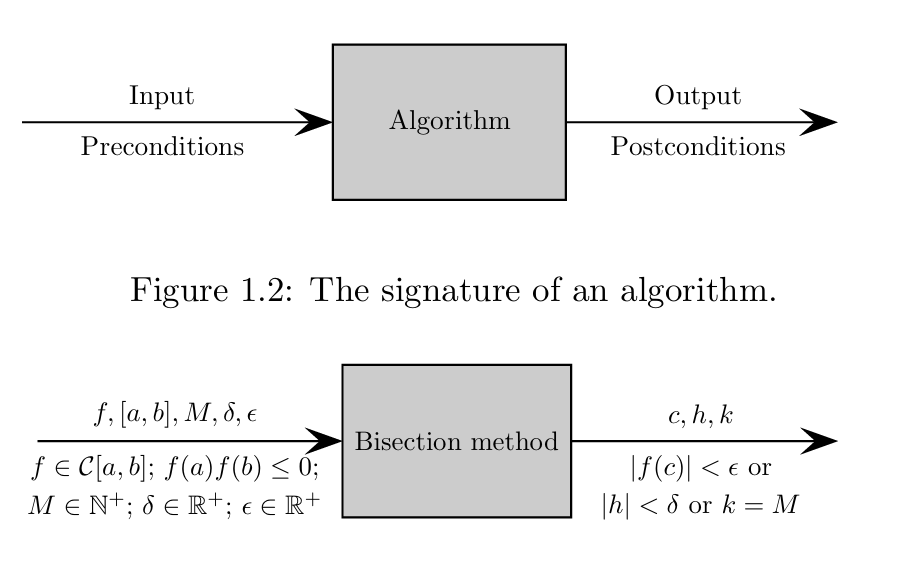
\includegraphics[width=0.75\textwidth]{images/algorithm_sign.png} % Replace with actual diagram if needed
\caption{算法的签名结构图}
\label{fig::signature}
\end{figure}

\begin{remark}
    % remark 1.3
    \label{rem::contract}
一个算法,就像一个定理,可以被看作是一个\textbf{契约(contract)}:它表示“只要你(用户)给予满足前提条件的输入,我(开发者)就会给你满足后置条件的输出。” 
一个算法可以如图~\ref{fig::signature} 所示地形式化表示。例如,二分法如图~\ref{fig::bisection} 所示。

契约,或者说断言。在定理场合,只要前提条件成立,结论就成立;在算法场合,只要输入符合前置条件,算法就会产生符合后置条件的输出。
\end{remark}

\begin{remark}
    % remark 1.4
如果先决条件被违反,算法的行为或输出将是未定义的。为了确保先决条件成立,我们可以在算法内部显式地检查它们(通常用关键字 \textbf{check} 表示),
或者将此责任转交给用户(通常用关键字 \textbf{require} 表示)。

在测试程序时,其本质是:在输入满足先决条件的测试用例后,验证后置条件是否成立。

定理需要被证明,而理论上讲,一个算法作为一个断言,也是可以被证明的,或者,作为在一个有限精度计算机上的程序,可以被测试,甚至被遍历测试。
\end{remark}

\begin{definition}
算法的签名由以下部分组成:输入、输出、前置条件、后置条件,以及对不满足前置条件的输入参数的处理方式。
\end{definition}

\begin{remark}
一个算法的签名从“黑箱”的外部唯一地决定了它的行为。
\end{remark}


\subsection{算法的正确性证明与简化}

\begin{definition}
\textbf{不变量}(invariant)是指在算法执行过程中始终成立的条件。
\end{definition}

\begin{remark}
算法的三个基本构建模块是:顺序执行的简单语句、条件语句,以及循环语句。我们特别关注的是那些在循环过程中保持不变的不变量。
\end{remark}

\begin{definition}
若某个变量在循环体内初始化,则称其为\textbf{临时变量}或\textbf{派生变量};若某个变量在进入循环之前就已初始化,并在不同迭代中保持其值的变化,
则称其为\textbf{持久变量}或\textbf{主变量}。    
\end{definition}

\begin{exercise}
算法 \ref{alg::bisection} 中的不变量有哪些?变量 \(a, b, c, h, u, v, w\) 各自表示什么?哪些是主变量?哪些是临时变量?请画出图示来说明这些变量的生命周期。    
\end{exercise}

\begin{remark}
为了证明一个算法的正确性,我们必须说明:
\begin{itemize}
  \item 算法在有限时间内终止;
  \item 输出满足后置条件。
\end{itemize}

第二点通常通过主变量的不变量,以及派生变量对主变量的依赖关系来证明。
\end{remark}

\begin{remark}
针对备注 \ref{rem::contract} 中的类比,我们关注的是黑箱的外部。事实上,该类比也适用于黑箱的内部,
含义如下:就像我们在证明定理时不需要无关或冗余的参数一样,我们也应尽可能简化算法。
\end{remark}

\begin{algorithm}
    % alg 1.9
    \label{alg::simple_bisection}
简化的二分法算法:

\begin{minipage}{0.45\textwidth}
\textbf{输入:} \\
$f : [a,b] \rightarrow \mathbb{R}$,$a \in \mathbb{R}$,$b \in \mathbb{R}$ \\
$M \in \mathbb{N}$,$\delta \in \mathbb{R}^+$,$\epsilon \in \mathbb{R}^+$ \\
\textbf{前提条件:} \\
$f \in C([a,b])$, $\text{sgn}(f(a)) \neq \text{sgn}(f(b))$ \\
\textbf{输出:} $c, h, k$ \\
\textbf{后置条件:} $|f(c)| < \epsilon$ 或 $|h| < \delta$ 或 $k = M$
\end{minipage}

\begin{enumerate}
\item $h \leftarrow b - a$
\item $u \leftarrow f(a)$
\item \textbf{for} $k = 0$ \textbf{to} $M$
\item \quad $h \leftarrow h / 2$
\item \quad $c \leftarrow a + h$
\item \quad \textbf{if} $|h| < \delta$ 或 $k = M$ \textbf{then break}
\item \quad $w \leftarrow f(c)$
\item \quad \textbf{if} $|w| < \epsilon$ \textbf{then break}
\item \quad \textbf{else if} $\text{sgn}(w) = \text{sgn}(u)$ \textbf{then}
\item \qquad $a \leftarrow c$
\item \textbf{end for}
\end{enumerate}
    
\end{algorithm}

\begin{remark}
如果将第 2 行放置在循环开始之后的位置,将更容易证明算法 \ref{alg::simple_bisection} 的正确性。
在这种情况下,证明可以基于以下两点:
\begin{enumerate}
    \item 观察到只有变量 \(a\) 是主变量,其他变量都是由 \(a\) 推导而来;
    \item 区间长度在每次迭代中都会缩小为原来的一半,这构成了一个不变量。
\end{enumerate}
此外,将第 2 行放在循环外并不会影响算法的正确性,因为在循环中我们只需要用到 \(f(a)\) 的符号。
\end{remark}

\begin{remark}
    % rem 1.10
    \label{rem::reduce_cost}
第 2 行留在循环之外的另一个重要原因是:计算非线性函数 \(f\) 可能代价较高。换句话说,我们应尽量减少在二分法循环中对 \(f\) 的求值。

事实上,只有当算法 \ref{alg::bisection} 和算法 \ref{alg::simple_bisection} 在循环中对 \(f\) 的求值次数相同,
它们在效率上才具有可比性。这也是两个算法中第 6 行的条件语句为何要与第 8 行分开的原因。
\end{remark}

\begin{remark}
算法 \ref{alg::simple_bisection} 相较于算法 \ref{alg::bisection},有哪些方面更加简单?
总的代码行数并不重要,一个更好的衡量方式是主变量的数量:算法 \ref{alg::bisection} 有四个主变量,而算法 \ref{alg::simple_bisection} 只有两个。

此外,算法 \ref{alg::simple_bisection} 中的主变量 \(h\) 是非常可预测的(在每次循环中都除以 $2$),
因此我们实际上只有一个主变量在语法结构和语义上都真正重要。
\end{remark}


\subsection{Q-阶收敛性}
% subsec 1.4
\label{subsec::Q_convergence}

\begin{definition}
    % def 1.10
    \label{def::Q_convergence}
(Q-阶收敛性)一个收敛序列 \(\{x_n\}\) 若满足以下条件,则称其以 Q-阶 \(p\)(其中 \(p \ge 1\))收敛于 \(L\):
\begin{equation}
\lim_{n \to \infty} \frac{|x_{n+1} - L|}{|x_n - L|^p} = c > 0
\end{equation}
其中常数 \(c\) 被称为\textbf{渐近因子(asymptotic factor)}。特别地:
\begin{itemize}
    \item 若 \(p = 1\),称为\textbf{线性收敛};
    \item 若 \(p = 2\),称为\textbf{二次收敛}。
\end{itemize}    
\end{definition}

\begin{remark}
收敛阶衡量的是收敛的速度。然而,只有当一个数列被证明确实收敛时,我们才能称其具有 $Q$ 阶收敛。换句话说,
定义 \ref{def::Q_convergence} 并不保证收敛,它仅仅衡量收敛的速度。

以求解 \( f(x) = \sin(x) = 0 \) 且 \( x \) 接近 $3$ 的情形为例。
如果渐近因子 \( c = 0.1 \), 那么线性收敛方法的每一次迭代将带来一位新的有效数字。如果 \( c = \frac{1}{2} \),
那么线性收敛方法的每次迭代将带来一位新的有效比特。对于二次收敛方法,每次迭代大致会使正确的数字或比特数翻倍。
\end{remark}

\begin{definition}
    % def 1.11
    \label{def::linear_convergence}
序列 \(\{x_n\}\) 若满足:
\begin{equation}
    % eq 1.2
    \label{eq::linear_convergence}
\exists c \in (0, 1), \exists d > 0, \text{使得 } \forall n \in \mathbb{N}, \quad |x_n - L| \le c^n d
\end{equation}
则称其\textbf{线性收敛于} \(L\).

若收敛序列 \(\{x_n\}\) 满足:
\begin{equation}
    % eq 1.3
    \label{eq::Q_convergence}
\exists c > 0, \exists N \in \mathbb{N}, \text{使得 } \forall n > N, \quad |x_{n+1} - L| \le c|x_n - L|^p
\end{equation}
则称其具有 \(p\) 阶收敛。  
\end{definition}

\begin{remark}
定义 \ref{def::linear_convergence} 可由定义 \ref{def::Q_convergence} 推出。(请使用定义 C.3 来证明这一点!)

请注意,(\ref{eq::linear_convergence}) 同时也保证了收敛性,而 (\ref{eq::Q_convergence}) 并不保证。例如,数列 \(\{1, -1, 1, -1, \dots\}\) 
满足 (\ref{eq::Q_convergence}) 中 \(L = 0\)、\(p = 1\)、\(c = 1\) 的条件,但该数列并不收敛。

(\ref{eq::linear_convergence}) 保证收敛性的关键在 于 \(c < 1\),而 (\ref{eq::Q_convergence}) 中的 \(c\) 可以大于 $1$.
\end{remark}

\begin{theorem}
(单调收敛定理)任何有界的单调序列都是收敛的。
\end{theorem}

\begin{theorem}
    % thm 1.13
    \label{thm::bisection}
(二分法的收敛性)设函数 \(f : [a_0, b_0] \to \mathbb{R}\) 连续,且满足 \(\text{sgn}(f(a_0)) \neq \text{sgn}(f(b_0))\),则二分法中迭代序列的误差以因子 \(\frac{1}{2}\) 线性收敛:
\begin{equation}
\lim_{n \to \infty} a_n = \lim_{n \to \infty} b_n = \lim_{n \to \infty} c_n = \alpha
\end{equation}
\begin{equation}
f(\alpha) = 0
\end{equation}
\begin{equation}
|c_n - \alpha| \le 2^{-n+1}(b_0 - a_0)
\end{equation}
其中 \([a_n, b_n]\) 表示第 \(n\) 次迭代的区间,\(c_n = \frac{1}{2}(a_n + b_n)\) 为当前迭代的中点。    
\end{theorem}

\begin{proof}
由算法定义可知:
\[
a_0 \le a_1 \le a_2 \le \cdots \le \alpha,\quad
b_0 \ge b_1 \ge b_2 \ge \cdots \ge \alpha
\]
\[
b_{n+1} - a_{n+1} = \frac{1}{2}(b_n - a_n)
\]
由单调收敛定理,\(\{a_n\}, \{b_n\}\) 均收敛,且区间长度趋于 $0$,因此中点也收敛于某个 \(\alpha\)。
由算法和初始条件可知,每次迭代区间内 \(f(a_n)f(b_n) \le 0\) 成立,故 \(f(\alpha) = 0\).
\end{proof}

\begin{remark}
请注意算法 \ref{alg::bisection} 的表示方式和循环\textit{不变量}是如何在定理 \ref{thm::bisection} 的证明中被利用的。
\end{remark}

\begin{remark}
二分法的优点包括:保证收敛、最终误差明确,并且易于并行计算。其缺点是收敛速度较慢,且在寻找满足 \( f(a)f(b) < 0 \) 的两个点 \(a, b\) 时可能存在困难。
这些观察基于一个事实:在许多实际情形中,我们可能并不知道函数 \(f(x)\) 的精确形式。
\end{remark}

\subsection{牛顿法}
\begin{remark}
    我们已经有二分法了,为何需要更多的方法?
\end{remark}

来看一个本质上快于二分法的求根算法, 因为它是 $Q$-二阶的, 而二分法是
$Q$-线性的. 它的来源是对 $f$ 在真解 $x^*$ 处做关于初值 $x_0$ 的 Taylor
展开, 并截断到第二项:
\begin{eqnarray*}
  &&0 = f(x^*)=f(x_0)+(x^* - x_0)f'(x_0) + o((x^* - x_0)^2) \\
  &\Rightarrow&f(x_0) + x^*f'(x_0) - x_0f'(x_0) \approx 0 \\
  &\Rightarrow&x^* \approx x_0 - \frac{f(x_0)}{f'(x_0)}.
\end{eqnarray*}
由此得到迭代公式.

\begin{figure}
\centering
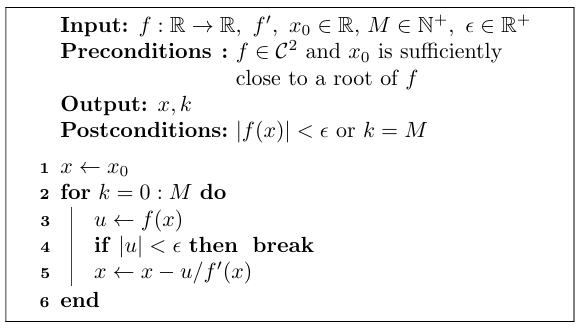
\includegraphics[width=0.75\textwidth]{images/newton_method.png}
\caption{牛顿法的步骤}    
\label{fig::newton}
\end{figure}

\begin{algorithm}
    % alg 1.14
    \label{alg::newton}
如图 \ref{fig::newton} 和 \ref{fig::geo_newton} 所示,牛顿法用于求解函数 \(f : \mathbb{R} \rightarrow \mathbb{R}\) 的根,从初始值 \(x_0\) 开始,使用迭代公式:
\begin{equation}
    % 
    \label{eq::newton}
x_{n+1} = x_n - \frac{f(x_n)}{f'(x_n)}, \quad n \in \mathbb{N}
\end{equation}
\end{algorithm}

\begin{remark}
一个函数的自变量可以包含另一个函数。这种特殊类型的函数被称为 \textit{泛函}(functional)或 \textit{函数子}(functor). 
在 \textbf{matlab} 中,函数子通过函数指针 \texttt{@} 实现;在 \textbf{C++} 中,函数子是具有 \texttt{operator()} 的类。
\end{remark}

\begin{remark}
牛顿法收敛得非常快,以至于在二分法中所需的停止准则 \(\delta\) 并不是必须的。
\end{remark}

\begin{figure}
\centering
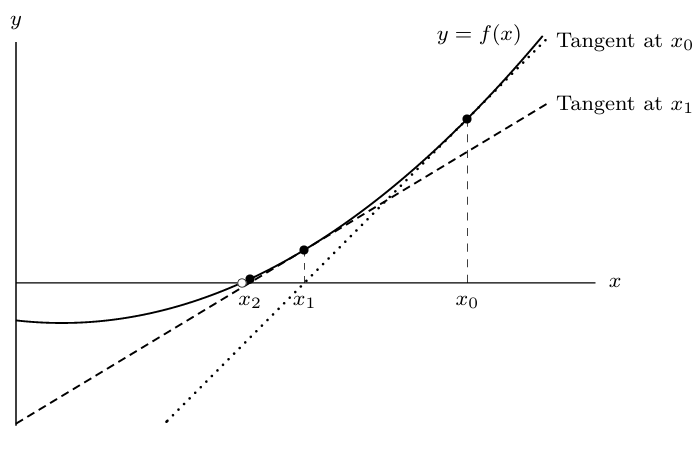
\includegraphics[width=0.75\textwidth]{images/geo_newton.png}
\caption{牛顿法的几何解释}
\label{fig::geo_newton}
\end{figure}

\begin{theorem}
    % 1.15
    \label{thm::newton}
(牛顿法的收敛性)  
设 \( f : \mathcal{B} \to \mathbb{R} \) 是定义在区间 \( \mathcal{B} = [\alpha - \delta, \alpha + \delta] \) 上的 \( C^2 \) 函数,
满足 \( f(\alpha) = 0 \) 且 \( f'(\alpha) \ne 0 \). 
若初始点 \( x_0 \) 足够接近根 \(\alpha\),则牛顿法生成的迭代序列 \(\{x_n\}\) 至少以\textbf{二次速度}收敛于 \(\alpha\),即:
\begin{equation}
\lim_{n \to \infty} \frac{\alpha - x_{n+1}}{(\alpha - x_n)^2} = \frac{f''(\alpha)}{2f'(\alpha)}.     
\end{equation}    
\end{theorem}

\begin{proof}
由泰勒公式(定理 C.99)和 \(f \in C^2\) 得:
\[
f(\alpha) = f(x_n) + (\alpha - x_n) f'(x_n) + \frac{(\alpha - x_n)^2}{2} f''(\xi)
\]
其中 \(\xi\) 在 \(x_n\) 与 \(\alpha\) 之间。因为 \(f(\alpha) = 0\),代入得:
\[
- \alpha = - x_n - \frac{f(x_n)}{f'(x_n)} + \frac{(\alpha - x_n)^2}{2} \frac{f''(\xi)}{f'(x_n)}
\]
即:
\[
x_{n+1} - \alpha = (x_n - \alpha)^2 \cdot \frac{f''(\xi)}{2f'(x_n)} \tag{*}
\]
由 \(f'(\alpha) \ne 0\) 的连续性可知,存在 \(\delta \in (0, \delta)\),使得在集合 
\(\mathcal{B}_1 = [\alpha - \delta_1, \alpha + \delta_1]\) 中,\(f'(x)\) 有界且不为零。
设:
\[
M := \frac{\max_{x \in \mathcal{B}_1} |f''(x)|}{2 \min_{x \in \mathcal{B}_1} |f'(x)|}
\]
若初始点 \(x_0\) 满足:
\begin{itemize}
    \item[(i)] \(|x_0 - \alpha| = \delta_0 < \delta_1\);
    \item[(ii)] \(M \delta_0 < 1\).
\end{itemize}
则根据 (*) 式可得:
\[
|x_{n+1} - \alpha| \le M |x_n - \alpha|^2
\]
所以收敛阶为 $2$. 并且由归纳法可得:
\[
|x_n - \alpha| \le \frac{1}{M} (M |x_0 - \alpha|)^{2^n}
\]
即 $x_n$ 收敛至 $\alpha$. 这证明了二次收敛性。若 \(f''(\alpha) = 0\),收敛速率可能高于二次。 
\end{proof}

\begin{remark}
短语 “至少”(at least)指的是超收敛情形,即 \( f''(\alpha) = 0 \). 
定理 \ref{thm::newton} 中模糊的表达 “足够接近”(sufficiently close)指的是其证明中条件 (i)、(ii),这两个条件必须同时满足。

换句话说,我们并没有一个逐步构造 \( x_0 \) 来满足这些条件的方法;我们甚至不会去尝试。
为什么?因为我们对函数 \( f \) 的信息不足。我们所能做的最好的事情,就是要求条件 (i)、(ii) 同时成立。
\end{remark}

\begin{remark}
牛顿法的主要优点是其收敛速度非常快。其缺点之一是需要我们知道导数 \( f'(x) \), 
而这可能难以获得,或者计算起来耗时较长。牛顿法的另一个主要缺点是我们无法判断初始点 \( x_0 \) 是否足够接近真实根。因此,收敛性无法得到保证。

例如,如果在定理 \ref{thm::newton} 的证明中条件 (i) 被违反,那么下一次迭代可能会远离根 \(\alpha\). 图 \ref{fig::newton_cond} 展示了条件 (ii) 的必要性。
\end{remark}

\begin{figure}
    % fig 1.6
    \label{fig::newton_cond}
\centering
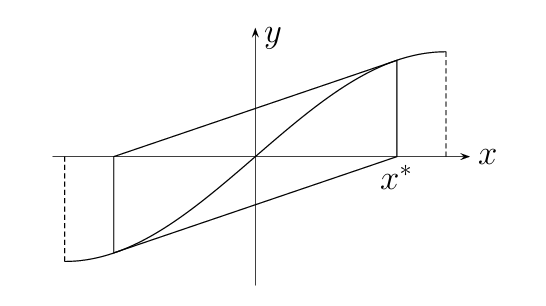
\includegraphics[width=0.5\textwidth]{images/newton_cond.png} % Replace with actual image
\caption{展示定理 \ref{thm::newton} 中条件必要性的特殊例子}
\end{figure}

\begin{theorem}
    % 1.16
    \label{thm::monotone}
若连续函数 \(f: [a,b] \to [c,d]\) 是双射,当且仅当 \(f\) 是严格单调的。
\end{theorem}

\begin{remark}
定理 \ref{thm::monotone} 的充分性部分可以重述为:“如果函数 \( f : [a, b] \to [c, d] \) 是连续且严格单调的,那么它是双射(bijective)。”\\
但其逆命题并不成立。你能给出一个反例吗?
\end{remark}

\begin{remark}
我们注意到,由于缺乏对函数 \( f \) 的信息,牛顿法的收敛性无法得到保证。解决该问题的一种方法是对 \( f \) 施加更多条件;定理 \ref{thm::newton_monotone} 就是一个例子。
\end{remark}

\begin{theorem}
    % thm 1.17
    \label{thm::newton_monotone}    
若 \(f : \mathbb{R} \to \mathbb{R}\) 为 \(C^2\) 函数,满足:
\begin{itemize}
    \item \(f(\alpha) = 0\)
    \item \(f' > 0\), \(f'' > 0\)
    \item \(\alpha\) 是 \(f\) 的唯一根
\end{itemize}
则对于任意 \(x_0 > \alpha\), 牛顿法迭代序列 \(\{x_n\}\) 二次收敛于 \(\alpha\).    
\end{theorem}

\begin{proof}
由定理 \ref{thm::monotone} 可知,函数 \( f \) 是双射,因为 \( f \) 是连续且严格单调的。
由于 \( 0 \) 在其值域中,\( f \) 必有唯一根。在证明定理 \ref{thm::newton} 时,我们有:

\begin{equation}
    % eq 1.9
    \label{eq::newton_residual}
x_{n+1} - \alpha = (x_n - \alpha)^2 \cdot \frac{f''(\xi)}{2 f'(x_n)}. 
\end{equation}

进一步地,\( f' > 0 \) 且 \( f'' > 0 \) 意味着对所有 \( n > 0 \), 
都有 \( x_n > \alpha \). 由于 \( f \) 是严格递增的,意味着 \( f(x_n) > f(\alpha) = 0 \), 
对所有 \( n > 0 \) 成立。根据牛顿法的定义,

\[
x_{n+1} - \alpha = x_n - \alpha - \frac{f(x_n)}{f'(x_n)},
\]

因此序列 \( \{x_n - \alpha : n > 0\} \) 是严格单调递减的,且以 $0$ 为下界。
由定理 \ref{eq::secant} 可知,该序列收敛。

设 \( \lim_{n \to \infty} x_n = a \),两边对等式 (\ref{eq::newton}) 取极限得:

\[
a = a - \frac{f(a)}{f'(a)},
\]

由此可得 \( f(a) = 0 \). 由于 \( f \) 的根是唯一的,因此 \( a = \alpha \)。

二次收敛速率可使用等式 (\ref{eq::newton_residual}) 进行归纳证明,如同在定理 \ref{thm::newton} 中所做的那样。
\end{proof}

\begin{remark}
对牛顿迭代 \( (x_n)_{n \in \mathbb{N}} \) 唯一收敛于 \(\alpha\) 的证明如下。

假设数列 \(\{x_n\}\) 收敛于 \(\alpha + c\),其中 \(c > 0\) 为某个固定常数。定义:
\[
\delta = \frac{f(\alpha + c)}{f'(\alpha + c)}.
\]
将 \(f(\alpha + c)\) 在 \(\alpha\) 处展开为泰勒级数,结合 \(f'(\alpha + c) > 0\) 可知 \(\delta > 0\)。因为牛顿迭代 \(\{x_n\}\) 收敛,所以有:
\[
\forall \epsilon > 0,\ \exists N \in \mathbb{N},\ \text{使得} \ \forall n > N,\ |x_n - x_{n+1}| = \left| \frac{f(x_n)}{f'(x_n)} \right| < \epsilon,
\]
尤其当 \(\epsilon = \frac{1}{2} \delta\) 时成立。

另一方面,
\[
\left| x_n - x_{n+1} - \frac{f(\alpha + c)}{f'(\alpha + c)} \right|
\geq \left| x_n - x_{n+1} \right| - \left| \frac{f(\alpha + c)}{f'(\alpha + c)} \right|
> \delta - \frac{1}{2} \delta = \frac{1}{2} \delta = \epsilon.
\]

这与牛顿迭代 \(\{x_n\}\) 收敛于 \(\alpha + c\) 的假设矛盾。因此结合前面的推理,说明牛顿迭代 \(\{x_n\}\) 实际上收敛于 \(\alpha\),即 \(f\) 的唯一根。
\end{remark}

\begin{definition}
    % def 1.18
    \label{def::convex_set}
向量空间 \(V\) 的子集 \(\mathcal{U}\) 是凸集当且仅当:
\begin{equation}
\forall x, y \in \mathcal{U}, \forall t \in (0,1), \quad tx + (1 - t)y \in \mathcal{U} 
\end{equation}
即线段上的所有点都在集合中。    
\end{definition}

\begin{definition}
函数 \(f : \mathcal{U} \to \mathbb{R}\) 是凸函数当且仅当:

\begin{equation}
    % eq 1.11
    \label{eq::convex_function}
\forall x, y \in \mathcal{U}, \forall t \in (0,1), \quad f(tx + (1 - t)y) \le t f(x) + (1 - t) f(y) 
\end{equation}    
\end{definition}

若将 \ref{eq::convex_function} 中“\(\le\)”换为“\(<\)”,则称 \(f\) 为严格凸函数。


\begin{remark}
一个 \( C^2 \) 函数 \( f : I \to \mathbb{R} \) 是凸的,当且仅当 \( f'' \geq 0 \) 在区间 \( I \) 上成立。
我们现在可以看到,定理 \ref{thm::newton_monotone} 中对函数 \( f \) 的要求是严格单调性和严格凸性。
\end{remark}

\begin{remark}
牛顿法可以通过反函数定理 D.120 直接推广到非线性方程组的情形;参见备注 D.53。
\end{remark}

\subsection{割线法}

\begin{remark}
如前所述,计算导数 \( f'(x) \) 可能代价非常高。为了降低计算成本,我们可以重复利用 \( x_n \) 和 \( x_{n-1} \) 处的函数值来近似导数。
这正是弦截法(secant method)的核心思想,它通常具有较高的性价比。
\end{remark}

\begin{algorithm}
如图~\ref{fig::secant-alg} 所示,割线法用于在初始猜测 \( x_0, x_1 \) 附近求解函数 \( f : \mathbb{R} \to \mathbb{R} \) 的根,其迭代公式为:
\begin{equation}
    % eq 1.12
    \label{eq::secant}
x_{n+1} = x_n - f(x_n) \frac{x_n - x_{n-1}}{f(x_n) - f(x_{n-1})}, \quad n \in \mathbb{N}^+.
\end{equation}
    
\end{algorithm}

\begin{figure}
\centering
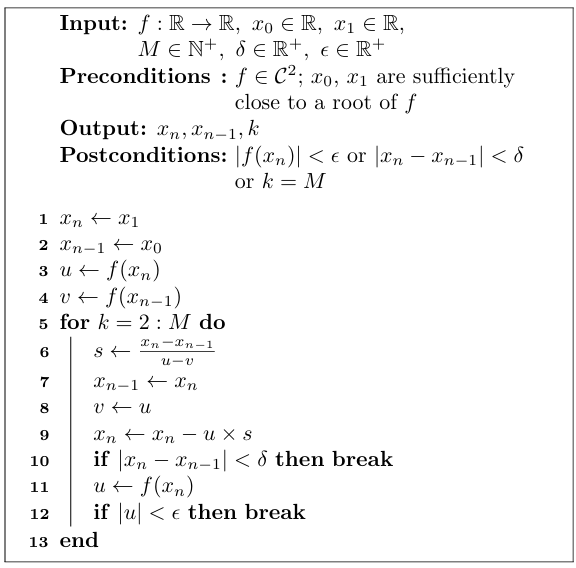
\includegraphics[width=0.75\textwidth]{images/secant_method.png} % 替换为实际图像
\caption{割线法算法}
\label{fig::secant-alg}
\end{figure}

\begin{remark}
我们将第 10 行的条件判断与第 12 行的分开,以减少对非线性函数的求值次数;参见备注 \ref{rem::reduce_cost}。
\end{remark}

\begin{definition}
    % 1.21
    \label{def::fibonacci}
斐波那契数列 \( \{F_n\} \) 定义为:
\begin{equation}
    % eq 1.13
    \label{eq::fibonacci}
F_0 = 0, \quad F_1 = 1, \quad F_{n+1} = F_n + F_{n-1}.
\end{equation}
\end{definition}

\begin{theorem}[Binet 公式]
    % 1.22
    \label{thm::binet}
设黄金比例为 \( r_0 = \frac{1+\sqrt{5}}{2} \),其共轭根为 \( r_1 = 1 - r_0 = \frac{1 - \sqrt{5}}{2} \),则斐波那契数列可表示为:
\begin{equation}
    % eq 1.14
F_n = \frac{r_0^n - r_1^n}{\sqrt{5}}.
\end{equation}
\end{theorem}

\begin{proof}
由定义 \ref{def::fibonacci} 可得:

令
\[
\mathbf{u}_k := 
\begin{bmatrix}
F_{k+1} \\
F_k
\end{bmatrix},
\quad
A := 
\begin{bmatrix}
1 & 1 \\
1 & 0
\end{bmatrix},
\]
则有 \( \mathbf{u}_k = A^k \mathbf{u}_0 \)。因此特征方程为:
\[
\det(A - \lambda I) = \lambda^2 - \lambda - 1 = 0
\]
其根为 \( r_0, r_1 \)。设对应特征向量为 \( \mathbf{x}_0, \mathbf{x}_1 \),则
\[
\mathbf{u}_0 = \frac{1}{r_0 - r_1} (r_0 \mathbf{x}_0 - r_1 \mathbf{x}_1)
\]
代入得结果。
\end{proof}

\begin{remark}
由于 \( r_0 \approx 1.618 \), \( r_1 \approx -0.618 \), 我们有
\[
\lim_{n \to +\infty} \left(F_n - \frac{r_0^n}{\sqrt{5}}\right) = 0.
\]
为了用浮点数计算 \( F_n \), 可以先计算 \( r_0^n / \sqrt{5} \), 再将结果四舍五入为最接近的整数以得到 \( F_n \). 
然而,这种方法可能比直接使用公式 (\ref{eq::fibonacci}) 计算慢得多。为什么?
\end{remark}

\begin{corollary}
    % 1.23
    \label{cor::fib_recurrence}
定理 \ref{thm::binet} 中的 \( r_0, r_1 \) 满足:
\begin{equation}
    % eq 1.15
F_{n+1} = r_0 F_n + r_1^n.
\end{equation}
\end{corollary}

\begin{lemma}[割线法误差表达式]
    % 1.24
    \label{lem::secant_error}
对于割线法(\ref{eq::secant}),存在 \( \xi_n \in (x_{n-1}, x_n) \), 
\( \zeta_n \in \big( \min(x_{n-1}, x_n, \alpha), \max(x_{n-1}, x_n, \alpha) \big) \), 使得:
\begin{equation}
    % eq 1.16
x_{n+1} - \alpha = (x_n - \alpha)(x_{n-1} - \alpha) \cdot \frac{f''(\zeta_n)}{2 f'(\xi_n)}.
\end{equation}
\end{lemma}

\begin{proof}
定义差商为:
\begin{equation}
    % eq 1.17
f[a,b] = \frac{f(a) - f(b)}{a - b}.
\end{equation}

代数变换可得公式等价为:
\begin{equation}
    % eq 1.18
x_{n+1} - \alpha = (x_n - \alpha)(x_{n-1} - \alpha) \cdot \frac{f[x_n, x_{n-1}] - f[x_n, \alpha]}{f[x_{n-1}, x_n]}.
\end{equation}

由平均值定理存在 \( \xi_n \in (x_{n-1}, x_n) \) 使得:
\begin{equation}
    % eq 1.19
f[x_{n-1}, x_n] = f'(\xi_n)
\end{equation}

定义 \( g(x) := f[x, x_n] \),再应用平均值定理,有:
\begin{equation}
    % eq 1.20
\frac{f[x_n, x_{n-1}] - f[x_n, \alpha]}{x_{n-1} - \alpha} = g'(\beta)
\end{equation}

对 \( g'(x) \) 求导并使用拉格朗日余项公式,有:
\begin{equation}
    % eq 1.21
\frac{f[x_n, x_{n-1}] - f[x_n, \alpha]}{x_{n-1} - \alpha} = \frac{f''(\zeta_n)}{2}
\end{equation}
代入即得结论。
\end{proof}

\begin{theorem}[割线法收敛性]
    % 1.25
    \label{thm::secant}
设函数 \( f : \mathcal{B} \to \mathbb{R} \) 为 \( C^2 \) 函数,
定义在区间 \( \mathcal{B} = [\alpha - \delta, \alpha + \delta] \) 上,
满足 \( f(\alpha) = 0 \)、\( f'(\alpha) \ne 0 \)、\( f''(\alpha) \ne 0 \),
若初始点 \( x_0, x_1 \) 足够接近 \(\alpha\),则割线法迭代序列 \( \{x_n\} \) 收敛于 \(\alpha\),其收敛阶为:
\begin{equation*}
    \label{eq::golden_ratio}
p = \frac{1 + \sqrt{5}}{2} \approx 1.618.
\end{equation*}
\end{theorem}

\begin{proof}
由于 \( f' \) 连续,且 \( f'(\alpha) \ne 0 \),可得存在 \( \delta_1 \in (0, \delta) \),
使得对所有 \( x \in \mathcal{B}_1 \subseteq \mathcal{B} \),有 \( f'(x) \ne 0 \).
其中 \( \mathcal{B}_1 = [\alpha - \delta_1, \alpha + \delta_1] \). 
定义 \( E_i = |x_i - \alpha| \),
\[
M = \frac{\displaystyle \max_{x \in B_1} |f''(x)|}{\displaystyle 2 \min_{x \in B_1} |f'(x)|}
\]
由引理 \ref{lem::secant_error} 可得:
\begin{equation*}
ME_{n+1} \leq ME_n ME_{n-1}.
\end{equation*}

选择初始点 \(x_0, x_1\) 满足:

\begin{enumerate}
    \item \( E_0 < \delta, \quad E_1 < \delta \);
    \item \( \max(ME_1, ME_0) = \eta < 1 \).
\end{enumerate}

则根据上述递推关系,可由归纳法证明:存在 \(\eta\) 使得所有 \( ME_n < \eta \). 记 \( ME_0 \leq \eta \),
 \( ME_1 \leq \eta \), 
 \( ME_2 \leq ME_1 ME_0 \leq \eta^2 \), 
 \( ME_3 \leq ME_2 ME_1 \leq \eta^3 \), $\cdots$, 
 \( ME_{n + 1} \leq ME_n ME_{n - 1} \leq \eta^{F_n + F_{n - 1}} = \eta^{F_n} \), 
 以此类推,得:
\[
E_n \leq B_n := \frac{1}{M} \eta^n.
\]
由定理 \ref{thm::binet} 可得:
\[
q_n \to \frac{1.618^{n+1}}{\sqrt{5}},
\]
从而 \( \lim_{n \to \infty} E_n = 0 \).

为了估计收敛速率,首先研究上界 \( \{B_n\} \) 的下降速度:

\begin{equation*}
\frac{B_{n+1}}{B^{r_0}_n} = \frac{\left(\frac{1}{M}\right)\eta^{F_{n+1}}}{\left(\frac{1}{M}\right)^{r_0}\eta^{r_0F_{n}}} 
= M^{r_0 - 1} \eta^{F_{n + 1} - r_0 F_n} \leq M^{r_0 - 1} \eta^{-1},
\end{equation*}
注意由推论 \ref{cor::fib_recurrence}  \( F_{n+1} - r_0 F_n = r_1^{n} \to -1 \). 

为证明收敛速率,我们定义:
\begin{equation}
    % eq 1.22
m_n := \frac{f''(\zeta_n)}{2f'(\xi_n)}, \quad m_\alpha := \left| \frac{f''(\alpha)}{2f'(\alpha)} \right|,
\end{equation}

其中 \( \zeta_n, \xi_n \) 与引理 \ref{lem::secant_error} 中相同。

通过归纳法,我们有:
\begin{align*}
E_n &= E_1^{{F_n}} E_0^{{F_{n-1}}} m_1^{F_{n-1}} \cdots m_{n-1}^{F_1}, \\
E_{n+1} &= E_1^{F_{n+1}} E_0^{F_n} m_1^{F_n} \cdots m_n^{F_1},
\end{align*}

其中 \( F_n \) 是定义 \ref{def::fibonacci} 中的斐波那契数列。于是,

\begin{equation}
    % eq 1.23
    \begin{array}{rcl}
\frac{E_{n+1}}{E_0^{F_n}} &=& E_1^{F_{n+1} - r_0 F_n} E_0^{F_n - r_0 F_{n-1}} m_1^{F_n - r_0 F_{n-1}} \cdots m_n^{F_1 - r_0 F_0}, \\
&=& E_1^{F_{n+1} - r_0 F_n} E_0^{F_n - r_0 F_{n-1}} \prod_{j=1}^n m_j^{F_{n+1-j} - r_0 F_{n-j}}, \\
&=& E_1^{r_1^{n-1}} E_0^{r_1^{n-2}} \cdots m_1^{r_1^1} m_n^{r_1^n}.
    \end{array}
\end{equation}

由推论 \ref{cor::fib_recurrence} 可得:

% \begin{equation}
%     % eq 1.24
% \lim_{n \to \infty} \frac{E_{n+1}}{E_0^{F_n}} = \lim_{n \to \infty} A \cdot \lim_{n \to \infty} B 
% = \lim_{n \to \infty} B \leq 2^{r_1 + r_1^2 + \cdots} \cdot \frac{1}{m_\alpha^0}.
% \end{equation}

\begin{equation}
    % eq 1.24
\lim_{n \to \infty} m_n = m_\alpha,
\end{equation}

于是存在常数 \( N \in \mathbb{N} \),使得对所有 \( n > N \),有:
\begin{equation}
    % eq 1.25
m_n \in \left( \frac{1}{2} m_\alpha, 2m_\alpha \right)
\end{equation}

定义:
\begin{equation*}
A := E_1^{r_1^{n-1}} E_0^{r_1^{n-2}} \cdots m_1^{r_1^1} m_2^{r_1^2} \cdots m_{N}^{r_1^N}
\end{equation*}

\begin{equation*}
B := m_{N+1}^{r_1^{N+1}} \cdots m_n^{r_1^n}
\end{equation*}

因此:
\begin{equation*}
\lim_{n \to \infty} B \leq 2^{\sum_{i=N+1}^{\infty} r_1^i} \cdot \frac{1}{m_\alpha^0}
\end{equation*}
\end{proof}

\begin{remark}
尽管牛顿法具有更高的收敛速度,弦截法可能计算代价更低。因此,对于一个给定的问题,我们应如何在牛顿法和弦截法之间做出选择?
如果我们 \textit{事先} 知道所需解的精度,那就选择 \textbf{CPU 时间更少} 的方法。
\end{remark}

\begin{corollary}
    % 1.26
    \label{cor::newton_secant_time}
若考虑 \( f(x) = 0 \) 在 \( x = \alpha \) 处的根,记 \( m \) 和 \( sm \) 分别为评估 \( f(x) \) 与 \( f'(x) \) 所需的时间,则达到所需精度所需的最短迭代次数分别为:

\begin{equation}
    % eq 1.26
    \label{eq::newton_secant_time}
T_N = (1 + s)m \lceil \log_2 K \rceil,
\end{equation}

\begin{equation}
    % eq 1.27
T_S = m \lceil \log_{r_0} K \rceil + m,
\end{equation}

其中:
\begin{equation*}
r_0 = \frac{1 + \sqrt{5}}{2}, \quad c = \left| \frac{f''(\alpha)}{2f'(\alpha)} \right|,
\end{equation*}

\begin{equation}
    % eq 1.28
K = \frac{\log c}{\log |x_0 - \alpha|},
\end{equation}

符号 \( \lceil \cdot \rceil \) 表示向上取整。
\end{corollary}

\begin{proof}
在定理 \ref{thm::newton} 中我们已证明 \( |x_n - \alpha| \leq \frac{1}{M} (ME_0)^{2^n} \), 令 \( E_n = |x_n - \alpha| \), 则有:
\[
ME_n \leq (ME_0)^{2^n}
\]

设 \( i \in \mathbb{N} \) 为最小次数使得误差满足 \( (ME_0)^{2^i} \leq M\epsilon \). 当 \( \epsilon \) 足够小时,\( M \to c \), 因此:

\[
i = \lceil \log_2 K \rceil
\]

对于牛顿法,每轮迭代需要一次函数和导函数评估,总耗时 \( (1 + s)m \). 因此有公式 (\ref{eq::newton_secant_time})。

对于割线法,假设 \( ME_0 \geq ME_1 \)。由定理 \ref{thm::secant} 可得:

\[
ME_n \approx (ME_0)^{\frac{\sqrt{5}}{2} r_0^{n+1}}
\]

忽略指数中的 \( -\frac{\sqrt{5}}{2} r_1^{n+1} \) 项。设 \( j \in \mathbb{N} \) 为最小迭代次数使得误差满足 \( r_0^{\sqrt{5} j} \leq K \), 因此:

\[
j = \left\lceil \frac{\log_{r_0} K + \log_{r_0} \sqrt{5}}{\sqrt{5}} \right\rceil = \lceil \log_{r_0} K \rceil + 1.
\]

由于割线法中初始值 \(x_0\) 和 \(x_1\) 已给出,因此最少迭代次数为 \(\lceil \log_{r_0} K \rceil\)(可与牛顿法比较!)。
此外,由于前一次迭代中已计算 \(f(x_{n-1})\),因此每次迭代仅需计算函数值 \(f(x_n)\)。最后,额外的项 \(m\) 是因为在第一次迭代中还需要计算 \(f(x_0)\).
\end{proof}

\begin{remark}
根据推论 \ref{cor::newton_secant_time},当比值 \( T_S / T_N < 1 \) 时,弦截法比牛顿法更快。这意味着
\[
s > \frac{\log 2}{\log r_0} - 1 \approx 0.44.
\]
\end{remark}

\subsection{不动点迭代}
% subsec 1.7

\begin{definition}
    % 1.27
一个函数 \( g \) 的\textbf{不动点} 是满足 \( g(\alpha) = \alpha \) 的自变量 \(\alpha\).
\end{definition}

\begin{example}
    % 1.28
函数 \( f(x) = x^2 - 3x + 4 \) 的不动点是 \( x = 2 \).
\end{example}

\begin{remark}
对于函数 \( f \) 的一个不动点,我们有
\[
f^n(x) := f(f(\cdots f(x))) = x,
\]
对任意 \( n \in \mathbb{N}^+ \) 成立。因此,这个名称由此而来。
\end{remark}

\begin{lemma}
    % 1.29
    \label{lem::fixed_point}
若 \( g : [a, b] \to [a, b] \) 连续,则 \( g \) 至少在区间 \([a, b]\) 上有一个不动点。
\end{lemma}

\begin{proof}
函数 \( f(x) = g(x) - x \) 满足 \( f(a) \geq 0 \)、\( f(b) \leq 0 \),由介值定理得证。
\end{proof}

\begin{exercise}
    % 1.30
    \label{exe::no_fixed_point}
设 \( A = [-1, 0) \cup (0, 1] \). 给出一个连续函数 \( g : A \to A \), 使其没有不动点。
再给出一个从 \( \mathbb{R} \to \mathbb{R} \) 的连续函数,其同样没有不动点。
\end{exercise}

\begin{remark}
引理 \ref{lem::fixed_point} 和习题 \ref{exe::no_fixed_point} 表明:若一个连续函数的定义域和值域是相同的集合 \( A \), 
在 \( A \) 满足某些条件时,该函数就会有不动点。那么,这些条件是什么呢?布劳威尔不动点定理为我们提供了一些线索。
\end{remark}

\begin{theorem}[Brouwer 不动点定理]
    % 1.31
    \label{thm::brouwer}
设 \( \mathbb{D}^n := \{ x \in \mathbb{R}^n : \|x\| \leq 1 \} \), 则任意连续函数 \( f : \mathbb{D}^n \to \mathbb{D}^n \) 至少有一个不动点。
\end{theorem}

\begin{proof}
见 Milnor [1978]。
\end{proof}

\begin{example}
    % 1.32
将一张地图放在地板上,设函数将地图上的每个点映射到其在地图上的对应位置。若地图是 \( \mathbb{D}^2 \) 的同胚映射,则存在某个点刚好映射到其在地面上的位置。
\end{example}

\begin{exercise}
    % 1.33
将两张相同大小的纸重叠放置,然后揉皱上面的一张纸并压在下面的一张上,证明至少存在一个点在揉皱后仍位于原处。
\end{exercise}

\begin{definition}
    % 1.34
\textbf{不动点迭代} 是通过如下形式迭代寻找不动点的方法:
\begin{equation}
    % eq 1.29
    \label{eq::fixed_point_iteration}
x_{n+1} = g(x_n), \quad n \in \mathbb{N}.
\end{equation}
\end{definition}

\begin{example}
    % 1.35
牛顿法就是一种不动点迭代。
\end{example}

$$
x_{n + 1} = x_n - \frac{f(x_n)}{f'(x_n)},
$$
所以牛顿法的迭代函数为
$$
g(x) = x - \frac{f(x)}{f'(x)}.
$$
它的不动点就是原方程 \( f(x) = 0 \) 的根。



\begin{exercise}
    % 1.36
    \label{exe::fixed_point_behavior}

为计算某个正实数 \( a \) 的平方根,我们可以将问题表述为求函数  
\[f(x) = x^2 - a\]  
的根。  
当 \( a = 1 \), 初始猜测值 \( x_0 = 2 \), 且有以下三种选择:  
\[g_1(x) := x^2 + x - a,\]  
\[g_2(x) := \frac{a}{x},\]  
以及  
\[g_3(x) := \frac{1}{2}\left(x + \frac{a}{x}\right),\]  

这三种形式都是和 $f(x) = 0$ 等价的形式,但可以验证 \( g_1 \) 发散,\( g_2 \) 振荡,\( g_3 \) 收敛。
本节中的定理将解释其原因。
\end{exercise}

\begin{definition}
    % 1.37
    \label{def::contraction}
若函数 \( f : [a, b] \to [a, b] \) 存在 \( \lambda \in [0, 1) \) 使得对任意 \( x, y \in [a, b] \) 有:
\begin{equation}
|f(x) - f(y)| \leq \lambda |x - y|,
\end{equation}
则称 \( f \) 为\textbf{压缩映射(contraction mapping)}。
\end{definition}

\begin{example}
    % 1.38
任意线性函数 \( f(x) = \lambda x + c \),其中 \( 0 \leq \lambda < 1 \),是压缩映射。
\end{example}

\begin{theorem}[压缩映射收敛定理]
    % 1.39
    \label{thm::contraction}
若 \( g(x) \) 是区间 \([a, b]\) 上的压缩映射,则它在 \([a, b]\) 内有唯一的不动点 \( \alpha \). 并且,迭代公式
\[
x_{n+1} = g(x_n)
\]
对于任意初始值 \( x_0 \in [a, b] \) 都收敛于 \( \alpha \),且有误差估计:
\begin{equation}
    % eq 1.31
    \label{eq::contraction_error}
|x_n - \alpha| \leq \frac{\lambda^n}{1 - \lambda} |x_1 - x_0|.
\end{equation}
\end{theorem}

\begin{proof}
由引理 \ref{lem::fixed_point} 知,$g$ 在区间 $[a,b]$ 上至少有一个不动点。设存在两个不同的不动点 $\alpha$ 与 $\beta$, 则
\[
|\alpha-\beta|=|g(\alpha)-g(\beta)|\le \lambda |\alpha-\beta|,
\]
这推出 $|\alpha-\beta|\le 0$, 亦即这两个不动点必相同。

由定义 \ref{def::contraction},$x_{n+1}=g(x_n)$, 从而所有 $x_n$ 都落在 $[a,b]$ 中。
为证明收敛性,注意到
\[
|x_{n+1}-\alpha| = |g(x_n)-g(\alpha)| \le \lambda |x_n-\alpha|.
\]
由归纳法并结合三角不等式,得到
\[
\begin{aligned}
|x_n-\alpha|
&\le \lambda^n |x_0-\alpha| \\
&\le \lambda^n\bigl(|x_1-x_0|+|x_1-\alpha|\bigr) \\
&\le \lambda^n\bigl(|x_1-x_0|+\lambda |x_0-\alpha|\bigr),
\end{aligned}
\]
从而推出
\[
|x_0-\alpha| \le \frac{1}{1-\lambda}\,|x_1-x_0|,
\]
并与式 (\ref{eq::contraction_error}) 一致。
\end{proof}

\begin{remark}
定理 \ref{thm::contraction} 不应与定理 \ref{thm::brouwer} 混淆。关于定理 \ref{thm::contraction} 的一个部分推广,可参见定理 D.118。
\end{remark}

\begin{remark}
有时判断一个函数是否为压缩映射是困难的。另一种方法是检查该函数的导数的绝对值是否 \textbf{处处小于 $1$}.
\end{remark}


\begin{theorem}
    % 1.40
    \label{thm::fixed_point_convergence}
设 $g:[a,b]\to [a,b]$。若 $g\in C^{1}[a,b]$ 且
\[
\lambda=\max_{x\in [a,b]}|g'(x)|<1,
\]
则 $g$ 在区间 $[a,b]$ 内有唯一的不动点 $\alpha$。此外,对任意初值 $x_0\in [a,b]$,不动点迭代式 (\ref{eq::fixed_point_iteration}) 都收敛到 $\alpha$, 
误差估计 (\ref{eq::contraction_error}) 成立,并且
\begin{equation}
    % eq 1.32
    \label{eq::fixed_point_derivative}
\lim_{n\to\infty}\frac{x_{n+1}-\alpha}{x_n-\alpha}=g'(\alpha).
\end{equation}
\end{theorem}

\begin{proof}
由中值定理(定理 C.91)可知,对所有 $x,y\in [a,b]$, 有
\[
|g(x)-g(y)|\le \lambda |x-y|.
\]
定理 \ref{thm::contraction} 给出了除式 (\ref{eq::fixed_point_derivative}) 之外的全部结论。
式 (\ref{eq::fixed_point_derivative}) 由
\[
x_{n+1}-\alpha=g(x_n)-g(\alpha)=g'(\xi)\,(x_n-\alpha),
\]
以及 $\lim_{n\to\infty}x_n=\alpha$ 与 $\xi$ 介于 $x_n$ 和 $\alpha$ 之间这一事实得到。
\end{proof}


\begin{corollary}
    % 1.41
    \label{cor::fixed_point_derivative_old}
设 $\alpha$ 是函数 $g:\mathbb{R}\to\mathbb{R}$ 的一个不动点,且 $|g'(\alpha)|<1$, 并且 $g\in C^{1}(\mathcal{B})$, 其中
\[
\mathcal{B}=[\alpha-\delta, \alpha+\delta]
\]
对某个 $\delta>0$. 若初值 $x_0$ 取得足够接近 $\alpha$, 则定理 \ref{thm::contraction} 的结论成立。
\end{corollary}

\begin{proof}
取 $\lambda$ 使得 $|g'(\alpha)|<\lambda<1$. 再取 $\delta_0\le \delta$, 使得在
\[
\mathcal{B}_0=[\alpha-\delta_0, \alpha+\delta_0]
\]
上有 $\max_{x\in \mathcal{B}_0}|g'(x)|\le \lambda<1$. 于是 $g(\mathcal{B}_0)\subset \mathcal{B}_0$. 应用定理 \ref{thm::fixed_point_convergence} 即得证。
\end{proof}

\begin{remark}
此时正是回到习题 \ref{exe::fixed_point_behavior} 并解释这三种方法的不同行为的好时机。
\end{remark}


\begin{corollary}
    % 1.42
    \label{cor::fixed_point_higher_order_old}
设 $g:[a,b]\to [a,b]$ 且在 $[a,b]$ 中有不动点 $g(\alpha)=\alpha$. 若
\begin{equation}
\left\{
\begin{aligned}
& g\in C^{p}[a,b],\\
& \forall k=1,2,\dots,p-1,\quad g^{(k)}(\alpha)=0,\\
& g^{(p)}(\alpha)\ne 0,
\end{aligned}
\right.
\end{equation}
并且初值 $x_0$ 取在足够接近 $\alpha$ 的位置,则不动点迭代式 (\ref{eq::fixed_point_iteration}) 以 $p$ 阶精度($p>1,\ p\in\mathbb{N}$)收敛到 $\alpha$.
\end{corollary}

\begin{proof}
由推论 \ref{cor::fixed_point_derivative_old} 得 $g'(\alpha)=0$. 由 $g'$ 的连续性,存在 $\delta>0$, 
使得不动点迭代在区间 $[\alpha-\delta,\alpha+\delta]$ 内唯一地收敛到 $\alpha$. 对 $g$ 在 $\alpha$ 处作泰勒展开,可得
\[
E_{\mathrm{abs}}(x_{n+1}) := |x_{n+1}-\alpha|
=|g(x_n)-g(\alpha)|
=\left|\sum_{i=1}^{p-1}\frac{(x_n-\alpha)^i}{i!}\,g^{(i)}(\alpha)
+\frac{(x_n-\alpha)^p}{p!}\,g^{(p)}(\xi)\right|
\]
其中某个 $\xi\in[a,b]$. 由于 $g^{(p)}$ 在 $[a,b]$ 上连续,由定理 C.70 知 $g^{(p)}$ 在 $[a,b]$ 上有界。故存在常数 $M$ 使得
\[
E_{\mathrm{abs}}(x_{n+1}) \le M\,E_{\mathrm{abs}}(x_n)^p.
\]
\end{proof}

\begin{example}
    % 1.43
下列方法具有三阶收敛性,用于计算 \( \sqrt{R} \):
\begin{equation}
x_{n+1} = \frac{x_n (x_n^2 + 3R)}{3x_n^2 + R}
\end{equation}

首先,\( \sqrt{R} \) 是函数
\begin{equation}
F(x) = \frac{x(x^2 + 3R)}{3x^2 + R}
\end{equation}
的不动点。

验证:
\begin{equation}
F(\sqrt{R}) = \frac{\sqrt{R}(R + 3R)}{3R + R} = \sqrt{R}
\end{equation}

其次,\( F(x) \) 的导数如下表:

% \begin{table}
% \centering
% \caption{函数 \( F(x) \) 的导数}
\begin{tabular}{@{}c|c|c@{}}
\toprule
\( n \) & \( F^{(n)}(x) \) & \( F^{(n)}(\sqrt{R}) \) \\
\midrule
1 & \( \dfrac{3(x^2 - R)^2}{(3x^2 + R)^2} \) & 0 \\
2 & \( \dfrac{48Rx(x^2 - R)}{(3x^2 + R)^3} \) & 0 \\
3 & \( \dfrac{-48R(9x^4 - 18Rx^2 + R^2)}{(3x^2 + R)^4} \) & \( \dfrac{-48R(-8R^2)}{(4R)^4} = \dfrac{3}{2R} \ne 0 \) \\
\bottomrule
\end{tabular}
% \end{table}

由推论 \ref{cor::fixed_point_higher_order_old} 可知,该方法具有三阶收敛性。
\end{example}

\begin{remark}
关于度量空间中压缩映射不动点的更一般结论,参见定理 D.118。关于求解非线性方程的更多方法,读者可参阅 Atkinson 所著的教材 \cite[第二章]{Atkinson1989Introduction}.
\end{remark}

\section{多项式插值}
% sec 2
\label{sec::polynomial_interpolation}

\begin{definition}
% def 2.1
    插值(Interpolation)是在一组已知离散数据点的取值范围内构造新的数据点,通常通过生成一条插值函数(interpolating function),其图像经过所有已知数据点。
\end{definition}

\begin{example}
% exp 2.2
    插值函数可以是分段常数、分段线性、多项式、样条,或其他非多项式函数。    
\end{example}

\begin{remark}
    % rem 2.1
用“契约”(contract)的语言表述,插值问题的输入是一系列插值条件对 $(x_i,f_i)$($i=0,1,\dots,n$), 输出为一个函数 $p$, 
满足后置条件 $p(x_i)=f_i$. 此外,我们还需要控制插值的不确定性,即确定在同时插值这些输入数据的两条平滑函数之间的最大差异。    
\end{remark}

\subsection{范德蒙行列式}

\begin{definition}
    % def 2.3
给定 $n$ 个参数 $t_1, t_2, \dots, t_n$, 相应的 $n\times n$ 范德蒙矩阵(Vandermonde matrix)$V$ 的第 $(i, j)$ 个元素为
\[
v_{i,j}=t_j^{\,i-1};
\]
以矩阵形式写为
\begin{equation}
    % eq 2.1
    \label{eq::vandermonde}
V(t_1,t_2,\dots,t_n)=
\begin{bmatrix}
1 & 1 & \cdots & 1 \\
t_1 & t_2 & \cdots & t_n \\
\vdots & \vdots & \ddots & \vdots \\
t_1^{\,n-1} & t_2^{\,n-1} & \cdots & t_n^{\,n-1}
\end{bmatrix}.
\end{equation}
\end{definition}

\begin{lemma}
    % lem 2.4
    \label{lem::vandermonde}
大小为 $(n+1)\times(n+1)$ 的范德蒙矩阵的行列式可表示为
\begin{equation}
    % eq 2.2
    \label{eq::vandermonde_determinant}
\det V(x_0,x_1,\dots,x_n)=
\prod_{i>j}(x_i-x_j).
\end{equation}    
\end{lemma}

\begin{proof}
考虑函数
\begin{equation}
    % eq 2.3
U(x)=\det V(x_0,x_1,\dots,x_{n-1},x)
=\begin{vmatrix}
1 & 1 & \cdots & 1 & 1\\
x_0 & x_1 & \cdots & x_{n-1} & x\\
\vdots & \vdots & \ddots & \vdots & \vdots\\
x_0^{\,n} & x_1^{\,n} & \cdots & x_{n-1}^{\,n} & x^{n}
\end{vmatrix}.
\end{equation}
显然,由行列式定义,$U(x)\in \mathbb{P}_n$, 并且在 $x_0,x_1,\ldots,x_{n-1}$ 处为零,因为将这些值代入 $x$ 会使行列式出现两列相同的列。

由此可得,$U(x)$ 是一个 $n$ 次多项式,并且 $x_0,x_1,\ldots,x_{n-1}$ 是它的 $n$ 个不同的根。因此,存在常数 $A$, 使得
\begin{equation*}
U(x)=A\prod_{i=0}^{n-1}(x-x_i),
\end{equation*}
其中常数 $A$ 仅依赖于 $x_0,x_1,\ldots,x_{n-1}$. 同时,对式中最后一列按代数余子式展开可知,$x^{n}$ 的系数等于 $\det V(x_0,x_1,\ldots,x_{n-1})$. 
于是
\begin{equation*}
U(x)=\det V(x_0,x_1,\ldots,x_{n-1})\prod_{i=0}^{n-1}(x-x_i),
\end{equation*}
从而得到递推关系
\begin{equation*}
\det V(x_0,x_1,\ldots,x_n)=\det V(x_0,x_1,\ldots,x_{n-1})\prod_{i=0}^{n-1}(x_n-x_i).
\end{equation*}
基于 $U(x_0,x_1)=x_1-x_0$ 的归纳法即可得到式 (\ref{eq::vandermonde_determinant}).
\end{proof}

\begin{remark}
(引理 \ref{lem::vandermonde} 的另一种证明)
对任意 $i=1,2,\ldots,n$ 与 $j<i$, 在范德蒙矩阵 (\ref{eq::vandermonde}) 中将 $x_i$ 用 $x_j$ 代换,可得 $\det V=0$. 
这样的代换总数为
\[
1+2+\cdots+n=\frac{n(n+1)}{2}.
\]
另一方面,$\det V$ 可被看作关于变量 $x_0,x_1,\ldots,x_n$ 的多项式。因此
\[
\prod_{i>j}(x_i-x_j)
\]
是 $\det V$ 的一个因子。由行列式的定义,$\det V$ 中每个多项式项的总次数也为
\[
1+2+\cdots+n=\frac{n(n+1)}{2}.
\]
注意到单项式 $x_1 x_2^{2}\cdots x_n^{n}$ 的系数为 $1$, 从而证明完成。
\end{remark}

\begin{theorem}[多项式插值的唯一性]
    % thm 2.5
    \label{thm::polynomial_interpolation}
给定互不相同的点 $x_0,x_1,\ldots,x_n\in\mathbb{C}$ 以及对应的函数值 $f_0,f_1,\ldots,f_n\in\mathbb{C}$. 
记 $\mathbb{P}_n$ 为次数不超过 $n$ 的多项式的集合。则存在唯一的多项式 $p_n(x)\in\mathbb{P}_n$, 使得
\begin{equation}
    % eq 2.4
    \label{eq::vandermonde_polynomial}
\forall i=0,1,\ldots,n,\qquad p_n(x_i)=f_i.
\end{equation}
\end{theorem}

\begin{proof}
设一个多项式 $\sum_{i=0}^{n} a_i x^{i}$, 其中有 $n+1$ 个待定系数 $a_i$. 条件 (\ref{eq::vandermonde_polynomial}) 导出如下含有 $n+1$ 个方程的线性方程组:
\begin{equation*}
a_0 + a_1 x_i + a_2 x_i^{2} + \cdots + a_n x_i^{n} = f_i,\qquad i=0,1,\ldots,n.
\end{equation*}
由引理 \ref{lem::vandermonde} 可知,该方程组的行列式为
\begin{equation*}
\prod_{i>j}(x_i-x_j).
\end{equation*}
由于各点互异,结合克拉默法则(定理 B.258)即得所求的唯一解。
\end{proof}

\begin{remark}
我们将在后续研究中利用插值多项式的唯一性。    
\end{remark}

\subsection{Cauchy 余项}
\begin{remark}
我们考虑一种很实际的情况. 用于插值输入的数据点, 来自一个
函数(已知或未知)的取值:
$$
y_i = f(x_i),
$$
这样我们相当于知道了 $f(x)$ 在 $x_i$ 的取值. 而对于 $x \neq x_i$,我
们可以用 $p_n(x)$ 去代替 $f(x)$. 也即我们相当于可以用一个容易计算的多
项式 $p_n(x)$ 去替代一个可能不容易计算, 甚至是没有解析表达式的函数. 
当然我们还没有讨论怎样构建这个 $p_n$ 的算法,
但不妨碍我们在知道存在唯一性的前提下,先问一下, 这样做多靠谱?    

为此我们需要有一些理论上的准备. 也就是定理 \ref{thm::generalized_rolle}. 
这是一个广义罗尔
(Generalized Rolle) 定理. 它的证明也只需要反复套用罗尔定理即可.
\end{remark} 

\begin{theorem}
    % thm 2.6
    \label{thm::generalized_rolle}
(广义 Rolle 定理). 设 $n \geq 2$. 
假设 $f \in C [a, b]$ 并且 $f^{(n)} (x)$ 在 $(a, b)$ 的每个点都存在。
假设对于 $a \leq x_0 < x_1 < \cdots < x_n \leq b$, 
有 $f (x_0) = f (x_1 ) = \cdots = f (x_n ) = 0$.
那么存在一个点 $\xi \in (x_0, x_n )$ 使得 $f^{(n)} (\xi) = 0$.    
\end{theorem}

\begin{proof}

\end{proof}
在 $n$ 个区间 $(x_i , x_{i+1} )$ 上应用 Rolle 定理(定理 C.90)
得到 $n$ 个点 $\zeta_i$, 在这些点上有 $f' (\zeta_i ) = 0$. 
考虑 $f' , f'' , \cdots , f^{(n-1)}$ 为新的函数。
反复应用上述论点完成证明。

定理 \ref{thm::generalized_rolle} 的一个重要应用在于定理 \ref{thm::cauchy_remainder}, 
即给出了用插值多项式 $p_n(x)$ 和被插函数 $f(x)$ 之间的误差估计
$$
R_n(f; x) : = f(x) - p_n(f; x)
= \frac{f^{(n + 1)}(\xi)}{(n + 1)!} \prod_{i = 0}^n (x - x_i).
$$

\begin{theorem}
    % thm 2.7
    \label{thm::cauchy_remainder}
(多项式插值的柯西余项) 设 $f \in C^{n} [a, b]$ 并且假设 $f^{(n+1)} (x)$ 
在 $(a, b)$ 的每个点都存在。让 $p_n (f ; x)$ 表示在 $P_n$ 中与 $f$ 
在 $x_0 , x_1 , \cdots , x_n$ 处取值相同的唯一多项式。
定义
\begin{equation}
    % eq 2.5
R_n (f ; x) := f (x) - p_n(f ; x) 
\end{equation}
为多项式插值的柯西余项。如果 $a \leq x_0 < x_1 < \cdots < x_n \leq b$, 
那么存在一些 $\xi \in (a, b)$ 使得
\begin{equation}
    % eq 2.6
    \label{eq::cauchy_remainder}
R_n (f ; x) = \frac{f^{(n+1)}(\xi)}{(n + 1)!} \prod_{i=0}^{n} (x - x_i) 
\end{equation}
其中,$\xi$ 的值依赖于 $x, x_0 , x_1 , \cdots , x_n$ 和 $f$.
\end{theorem}

\begin{proof}
由于 $f (x_k ) = p_n (f ; x_k )$, 余数 $R_n (f ; x)$ 在 $x_k$ 处为零。
固定 $x \neq x_0, x_1 , \cdots , x_n$ 并定义
\[
K(x) = \frac{f (x) - p_n (f ; x)}{\prod_{i=0}^{n} (x - x_i)}
\]
和一个关于 $t$ 的函数
\[
W (t) = f (t) - p_n (f ; t) - K(x) \prod_{i=0}^{n} (t - x_i).
\]
函数 $W (t)$ 在 $t = x_0, x_1, \cdots , x_n$ 处为零($K$ 后面的连乘)。
另外 $W (x) = 0$($K$ 分母消去)。
根据定理 \ref{thm::generalized_rolle},对于某些 $\xi \in (a, b)$, 
有 $W^{(n+1)} (\xi) = 0$, 即
\[
0 = W^{(n+1)} (\xi) = f^{(n+1)}(\xi) - (n + 1)!K(x).
\]
因此 $K(x) = f^{(n+1)} (\xi)/(n + 1)!$ 并且 (\ref{eq::cauchy_remainder}) 成立。
这是一个很像中值定理的结论和证明。
\end{proof}

\begin{corollary}
    % cor 2.8
    \label{cor::cauchy_remainder}
设 $f(x)\in C^{n+1}[a, b]$. 则有
\begin{equation}
    % eq 2.7
\lvert R_n(f;x)\rvert
\le \frac{M_{n+1}}{(n+1)!}\prod_{i=0}^{n}\lvert x-x_i\rvert
\le \frac{M_{n+1}}{(n+1)!}\,(b-a)^{n+1},
\end{equation}
其中
\begin{equation*}
M_{n+1}=\max_{x\in[a,b]}\bigl\lvert f^{(n+1)}(x)\bigr\rvert .
\end{equation*}
\end{corollary}

\begin{example}
    % exp 2.9
    \label{exp::arcsin}
通过对 $x=0.5330$ 与 $x=0.5340$ 两点作线性插值来近似 $\arcsin(0.5335)$. 估计由此产生的误差。

取 $f(x)=\arcsin(x)$. 则
\begin{equation*}
f''(x)=x(1-x^{2})^{-3/2},\qquad
f^{(3)}(x)=(1+2x^{2})(1-x^{2})^{-5/2}.
\end{equation*}
由于在区间 $[0.5330,\,0.5340]$ 上第三阶导数为正,$f''$ 的最大值出现在 $x=0.5340$. 
由上面的推论可得
\begin{equation*}
\lvert R_1\rvert \le 4.42\times 10^{-7}.
\end{equation*}
实际误差约为
\begin{equation*}
1.10\times 10^{-7}.
\end{equation*}
真正的误差大约是 $1.10 \times 10^{-7}$. 大家有没有注意到这就是查数学用表时的做法?
\end{example}

推论 \ref{cor::cauchy_remainder} 将误差界整理成两个更加清晰的形式, 特别是后一个界, 给出了
input 和 precondition 的现实意义:
$$
|R_n(f; x)| \leq
\frac{\max_{x \in [a, b]}\left|f^{(n + 1)}(x)\right|}{(n + 1)!}(b - a)^{n + 1}.
$$

例子 \ref{exp::arcsin} 给出了一个实际案例的估值.

\subsection{Lagrange 公式}
\begin{remark}
插值问题的理论模型是在空间 $\mathbb{P}_n$ 中寻找一个目标多项式:
$$
p_n(x) = \sum_{j = 0}^n a_j x^j
$$
满足
$$
p_n(x_i) = y_i.
$$
这里 $a_j$, $j = 0, 1, \cdots, n$ 是待定系数.

从线性代数的角度观察这个问题, 
对 $\mathbb{P}_n$ 的一组基:
$$
\left\{
\phi_0, \phi_1, \cdots, \phi_n,
\right\}
$$
则
$$
p_n(x) = \sum_{j = 0}^n a_j \phi_j(x),
$$
需满足
$$
p_n(x_i) = \sum_{j = 0}^n a_j \phi_j(x_i) = y_i.
$$
现在系数矩阵是 $\left[\phi_j(x_i)\right]$. 

如果我们选取了
$\mathbb{P}_n$ 的一组基:
$$
\left\{1, x, x^2, \cdots, x^n\right\}
$$
来表出插值多项式 $p_n(x)$, 
其实就是定理 \ref{thm::polynomial_interpolation} 得到的一个线性方
程组, 但系数矩阵是 Vandermonde 矩阵. 


而如果取 $\mathbb{P}_n$ 的另一组基
$$
\left\{\phi_j(x) = \prod_{j \neq i}\frac{x - x_j}{x_i - x_j}
\right\}, j = 0, 1, \cdots, n.
$$
满足
$$
\phi_j(x_i) = \left\{
\begin{array}{ll}
  1,& i = j \\
  0,& i \neq j.
\end{array}
\right.
$$
这组基, 我们称它为 Lagrange 插值基函数. 一般我们用 $l_j(x), j = 0, 1, \cdots, n$
表示(和书上公式 \ref{eq::lagrange_basis} 对上了). 在这组基下, 插值多项式
$$
p_n(x) = \sum_{j = 0}^n a_j l_j(x)
$$
满足 $p_n(x_i) = y_i$, $i = 0, 1, \cdots, n$,
则在这组基下,待定系数对应的线性方程组的系数矩阵是单位矩阵. 也就是说,
直接有 $a_i = y_i$. 于是我们可以直接写出
$$
p_n(x) = \sum_{j = 0}^n y_j l_j(x).
$$
这里注意, 由定理 \ref{thm::polynomial_interpolation}, 插值多项式是唯一的. 因此我们实际上只是给出了一个
得到 $p_n(x)$ 的更好的算法, 这个算法就是 Lagrange 插值公式. 也就是书上
的公式 \ref{eq::lagrange}.    
\end{remark}

\begin{definition}
    % def 2.10
    \label{def::lagrange}
为在互异点 $x_0,x_1,\ldots,x_n$ 处插值给定数值 $f_0,f_1,\ldots,f_n$, 拉格朗日(Lagrange)公式为
\begin{equation}
    % eq 2.8
    \label{eq::lagrange}
p_n(x)=\sum_{k=0}^{n} f_k\,\ell_k(x),
\end{equation}
其中用于点值插值的基函数(或称初等拉格朗日插值多项式)$\ell_k(x)$ 定义为
\begin{equation}
    % eq 2.9
    \label{eq::lagrange_basis}
\ell_k(x)=\prod_{\substack{i=0\\ i\ne k}}^{n}\frac{x-x_i}{x_k-x_i}.
\end{equation}
特别地,当 $n=0$ 时,$\ell_0\equiv 1$.
\end{definition}

可以验证两点式。

\begin{example}
    % exp 2.11
    \label{exp::lagrange}
对于 $i = 0, 1, 2$, 我们给出 $x_i = 1, 2, 4$ 和 $f (x_i ) = 8, 1, 5$. 
拉格朗日公式生成了 $p_2 (x) = 3x^2 - 16x + 21$.
    
\end{example}

我们还可以把 Lagrange 多项式写的更紧凑一些:

\begin{lemma}
    % lem 2.12
    \label{lem::lagrange_symmetric}
定义对称多项式
\begin{equation}
    % eq 2.10
    \label{eq::lagrange_symmetric}
\pi_n(x)=
\begin{cases}
1, & n=0,\\[4pt]
\displaystyle\prod_{i=0}^{n-1}(x-x_i), & n>0.
\end{cases}
\end{equation}
于是当 $n>0$ 时,点值插值的基函数可写为
\begin{equation}
    % eq 2.11
    \label{eq::lagrange_symmetric_basis}
\forall x\ne x_k,\qquad
\ell_k(x)=\frac{\pi_{n+1}(x)}{(x-x_k)\,\pi_{n+1}'(x_k)}.
\end{equation}

\begin{proof}
由链式法则,$\pi_{n+1}'(x)$ 是由 $n+1$ 项之和构成,每一项都是 $n$ 个因子的乘积。
当以 $x_k$ 代入 $x$ 时,这 $n+1$ 项除一项外全部为零,结论成立。
\end{proof}
\end{lemma}
(验证一下。)

\begin{remark}
定理 \ref{thm::polynomial_interpolation} 与定理 \ref{thm::cauchy_remainder} 表明:
对次数不超过 $k$ 的多项式插值算子作用在次数不超过 $k$ 的多项式 $q$ 上,结果正是 $q$ 本身。    
\end{remark}

由插值多项式唯一性, 定理 \ref{thm::generalized_rolle} 
和 \ref{thm::cauchy_remainder} 给出的余项和误差界都继续成立.

由于 $i \neq j$ 这个多少带有一点不对称性, 有时对我们的理论推导造成困难.
所以另外一种常用的对称形式的 Lagrange 插值基函数形式是课本的公式 (\ref{eq::lagrange_symmetric_basis}).
它需要用到引理 \ref{lem::lagrange_symmetric}, 在很多书上, $\pi_{n + 1}(x)$ 会用用一个更简略的记号
$\omega_{n + 1}(x)$ 甚至 $\omega(x)$ ($n$ 由上下文决定) 表示. 此时
Lagrange 插值基函数会写成:
$$
l_k(x) = \frac{1}{x - x_k}\frac{\omega(x)}{\omega'(x)}, k = 0, 1, \cdots, n.
$$

这里计算一下 $\pi_{n + 1}'(x_k)$

大家脑补一下 Lagrange 插值基函数应该长成什么样子? 画画看? 课本上的引理 \ref{lem::cauchy}, 也从
另一个角度给出其一个性质. 

Jupyer 画个图... Lagrange.pdf

\begin{lemma}(柯西(Cauchy)关系)
    % lem 2.13
    \label{lem::cauchy}
拉格朗日基函数 $\ell_k(x)$ 满足以下柯西关系:
\begin{equation}
    % eq 2.12
    \label{eq::cauchy}
\sum_{k=0}^{n}\ell_k(x)\equiv 1;
\end{equation}
\begin{equation}
    % eq 2.13
    \label{eq::cauchy_higher}
\forall\, j=1,\ldots,n,\qquad \sum_{k=0}^{n}(x_k-x)^{j}\,\ell_k(x)\equiv 0.
\end{equation}
\end{lemma}
\begin{proof}
由定理 \ref{thm::polynomial_interpolation} 与 \ref{thm::cauchy_remainder} 可知,
对每个 $q(x)\in\mathbb{P}_n$, 都有 $p_n(q;x)\equiv q(x)$. 
对常值函数 $f(x)\equiv 1$ 进行拉格朗日插值即得上式第一式。

类似地,令 $q_j(u):=(u-x)^j$, 其中 $x$ 为自由参数。于是对任意 $j=1,\ldots,n$, 有 (对 $u$ 做自变量插值)
\begin{equation*}
p_n(q_j;u)\equiv q_j(u)\quad \Rightarrow \quad \sum_{k=0}^{n}(x_k-x)^j\,\ell_k(u)\equiv (u-x)^j,
\end{equation*}
当令 $u=x$ 时便得到第二式。
\end{proof}

% 证明. 根据定理 2.5 和 2.7,对于每个 $q(x) \in P_n$,
% 我们都有 $p_n (q; x) \equiv q(x)$(即多项式的多项式插值就是自己)。
% 用拉格朗日公式插值常数函数 $f (x) \equiv 1$,得到 (2.12)。

% 同样,定义 $q_j (u) := (u - x)^j$,其中 $x$ 是一个自由参数,所以把它看成一个关于 $u$ 的多项式,
% 就是一个 $j$ 次的,进而对于任何 $j = 1, \cdots , n$,做关于 $u$ 的多项式插值,有
% \[
% p_n (q_j ; u) \equiv q_j (u) \Rightarrow \sum_{k=0}^{n} (x_k - x)^j \ell_k (u) \equiv (u - x)^j ,
% \]
% 注意第一个式子还是多项式的插值就是多项式本身,第二个式子是 $(u - x)^j$ 关于 $u$ 在 $x_k$ 点做 
% $n$ 次多项式插值
% \[
%   p_n(u) = \sum_{k=0}^{n} \left.(u - x)^j\right|_{u = x_k} \ell_k (u) = \sum_{k=0}^{n} (x_k - x)^j \ell_k (u).
% \]
% 最后当我们设定 $u = x$ 时,得到 (2.13)。


\begin{remark}
(柯西关系的另一种证明 ???)
设存在某个 $x=x_c$ 使得上述第二式不成立。对每个 $j=1,\ldots,n$, 
对多项式 $q(x)=(x-u)^j$ 作拉格朗日插值,得到
\begin{equation*}
(x-u)^j=p_n(q,x)=\sum_{k=0}^{n}q_k\,\ell_k(x)=\sum_{k=0}^{n}(x_k-u)^j\,\ell_k(x).
\end{equation*}
令 $u=x_c$ 即得矛盾。    
\end{remark}

\subsection{Newton 公式}
% subsec 2.4

\begin{remark}
Lagrange 插值公式非常漂亮, 理论上也很完美. 但它也有几个槽点:

\begin{enumerate}
\item 它的计算形式, 稳定性不是很好, 因此插值的次数不能太高, 比如不要超过 $20$;
\item Lagrange 插值公式是依赖插值数据 $(x_i, f_i)$ 的, 一旦数据发生变
  化, 则插值公式都需要重写. 之前的计算也全部白费. 一个常见的场景是, 我
  们取了 $6$ 个点的数据进行计算, 发现精度不够, 于是希望增加到 $7$ 个,
  然而我们需要重新计算全部基函数, 之前的计算也都全部无用. 
\end{enumerate}

应该说, Newton 公式并不是因为上述原因才产生的, 但它确实能解决上述问题.
这又是一个新的插值算法(多项式本身是唯一的).

我们注意到公式 (\ref{eq::lagrange_symmetric}) 给出的 $\pi_n(x)$ 其实是 $\mathbb{P}_n$ 空间的一组基: 
$$
\forall p_n(x) \in \mathbb{P}_n, p_n(x) = \sum_{k = 0}^n a_k \pi_k(x).
$$
%也就是课本的公式 \ref{eq::newton_interpolation}.

这一组基的特点是,
$$
\left\{\pi_0, \pi_1, \cdots, \pi_k\right\}
$$
即前 $k + 1$ 项, 就是子空间 $\mathbb{P}_k$ 的全部基. 那就意味着当空间从
$\mathbb{P}_n$ 扩展到$\mathbb{P}_{n + 1}$ 时, 全部增加的部分($x^{n + 1}项$),
都只和基函数 $\pi_{n + 1}$ 有关. 换言之, 当我们要求更高的插值精度, 也就是希望将插值函数从
$p_n(x)$ 提高到 $p_{n + 1}(x)$, 其实我们只要增加一项
$a_{n + 1}\pi_{n + 1}(x)$ 就行了, 或者说, 确定一下 $a_{n + 1}$ 是多少就可以了.

我们来讨论 $a_k$, $k = 0, 1, \cdots, a_n$
的具体形式:

首先, 如果我们只有一个数据 $(x_0, f_0)$, 那我们只能构建一个零次多项式:
$$
p_0(x) = a_0 \pi_0(x) = a_0. 
$$
它满足
$$
p_0(x_0) = a_0 = f_0.
$$
于是 $a_0$ 自然就有了.

接下去我们多了一个数据 $(x_1, f_1)$, 我们希望将 $p_0(x)$ 改进成一个一次多项式 $p_1(x)$:
$$
p_1(x) = a_0 \pi_0(x) + a_1 \pi_1(x) = p_0(x) + a_1 (x - x_0),
$$
我们注意到之间的计算结果 $p_0(x)$ 被自然包含入 $p_1(x)$, 而且
$$
p_1(x_0) = p_0(x_0) = f_0
$$
完全相容. 现在我们只需要考虑
$$
p_1(x_1) = f_0 + a_1 \pi_x(x_1) = f_0 + a_1 (x_1 - x_0) = f_1,
$$
也即
$$
a_1 = \frac{f_1 - f_0}{x_1 - x_0}.
$$
于是我们又得到了 $p_1(x)$.

令
$$
a_0 = f[x_0] := f(x_0), a_1 = f[x_0, x_1] := \frac{f_1 - f_0}{x_1 - x_0},
$$
以及
$$
a_k = f[x_0, x_1, \cdots, x_k],
$$
那我们怎么去探求它的一般形式呢? 以后我们称呼这种形式为 $f$ 关于点 $x_0, x_1, \cdots, x_k$
的 $k-$阶差商. 也有人把方括号放前面. 它可以理解为上述基下的插值多项式系数 $a_k$.
\end{remark}

\begin{definition}
    % def 2.14
    \label{def::newton_interpolating}
(差商和牛顿公式) 牛顿公式用于插值在不同点 
$x_0, x_1, \cdots , x_n$ 上的值 $f_0 , f_1 , \cdots , f_n$,公式为
\begin{equation}
    % eq 2.14
    \label{eq::newton_interpolation}
p_n(x) = \sum_{k=0}^{n} a_k \pi_k(x), 
\end{equation}
其中 $\pi_k$ 在 (\ref{eq::lagrange_symmetric}) 中定义,第 $k$ 个差商 $a_k$ 定义为 $p_k (f ; x)$ 中 $x^k$ 的系数,
并记作 $f [x_0 , x_1 , \cdots , x_k ]$ 或 $[x_0 , x_1 , \cdots , x_k ]f$.
特别地,有 $f [x_0 ] = f (x_0)$.
\end{definition}

\begin{remark}
差商 $a_i$ 是明确定义的:插值条件可以表示为一个上三角线性系统,
\[
\begin{bmatrix}
 \pi_0(x_0) & 0 & \cdots & 0 \\
 \pi_0(x_1) & \pi_1(x_1) & \cdots & 0 \\
 \vdots & \vdots & \ddots & \vdots \\
 \pi_0(x_n) & \pi_1(x_n) & \cdots & \pi_n(x_n) \\
\end{bmatrix} \begin{bmatrix}
 a_0 \\
 a_1 \\
 \vdots \\
 a_n \\
\end{bmatrix} = \begin{bmatrix}
 f (x_0) \\
 f (x_1) \\
 \vdots \\
 f (x_n) \\
\end{bmatrix},
\]
由此,通过前向替换,可以唯一确定 $a_i$,这要归功于 (\ref{eq::lagrange_symmetric}) 
引出的 $\pi_i(x_i) \neq 0$ 对于每个 $i = 0, 1, \cdots , n$ 都成立。
也要强调,在牛顿公式 (\ref{eq::newton_interpolation}) 中,每个 $\pi_k$ 对应 $k$ 个点,而每个 $a_k$ 对应 $k + 1$ 个点。

前向替换得到 $a_0 = f (x_0 )$ 和
\[
a_1 = \frac{f (x_1) - f (x_0)}{x_1 - x_0},
\]
这与定理 \ref{thm:DD-recursion} 一起,证明了 ``差商''这个名字的合理性。    
\end{remark}

在推出差商一般式之前,我们先观察一下差商的性质:

\begin{corollary}
    % cor 2.15
    \label{thm:DD-recursion_permutation}
(差商的对称性)
设 $(i_0,i_1,i_2,\ldots,i_k)$ 是 $(0,1,2,\ldots,k)$ 的一个排列。则
\begin{equation}
    % eq 2.15
    \label{eq::newton_permutation}
f[x_0,x_1,\ldots,x_k]=f[x_{i_0},x_{i_1},\ldots,x_{i_k}].
\end{equation}

\begin{proof}
插值多项式与插值节点的编号无关。其余部分由定理 \ref{thm::polynomial_interpolation} 中插值多项式的唯一性立即得到。
\end{proof}
\end{corollary}

\begin{corollary}
    % cor 2.16
    \label{cor::newton_explicit}
第 $k$ 个差商可表示为
\begin{equation}
    % eq 2.16
    \label{eq::newton_explicit}
f[x_0,x_1,\ldots,x_k]
=\sum_{i=0}^{k}\frac{f_i}{\displaystyle\prod_{\substack{j=0\\ j\ne i}}^{k}(x_i-x_j)}
=\sum_{i=0}^{k}\frac{f_i}{\pi_{k+1}'(x_i)},
\end{equation}
其中 $\pi_{k+1}(x)$ 定义见式(\ref{eq::lagrange_symmetric})。
\begin{proof}
由定理 \ref{thm::polynomial_interpolation} 的唯一性可知,式(\ref{eq::lagrange})与式(\ref{eq::newton_interpolation})所给出的两个多项式相同。
于是第一个等式由式(\ref{eq::lagrange_basis})与定义 \ref{def::newton_interpolating} 得到,而第二个等式由引理 \ref{lem::lagrange_symmetric} 得到。
\end{proof}
\end{corollary}


\begin{remark}
推论 \ref{thm:DD-recursion_permutation} 告诉我们, 对 $k-$阶差商, 交换这些结点的次序, 是没有关系的. 因为不论什么次序,
这 $k + 1$ 个结点唯一确定了插值多项式.

而和 Lagrange 插值公式对比一下, 不难得到推论 \ref{cor::newton_explicit} 的结论.

% 最后, 定理 \ref{thm:DD-recursion} 给出了 $k-$阶差商的递推公式, 这里的证明思路是:

% 记 $p_{k - 1}^{(1)}(x)$ 是 $(x_i, f_i)$, $i = 0, 1, \cdots, k - 1$ 下的插值多项式;
% 而 $p_{k - 1}^{(2)}(x)$ 是 $(x_i, f_i)$, $i = 1, \cdots, k$ 下的插值多项式;令
% $$
% p_k(x) = p_{k - 1}^{(1)}(x)
% + \frac{x - x_0}{x_k - x_0}\left(p_{k - 1}^{(2)}(x) - p_{k - 1}^{(1)}(x)\right),
% $$
% 则
% $$
% p_k(x_0) = p_{k - 1}^{(1)}(x_0) = f_0,
% $$
% 而
% $$
% p_k(x_i) = p_{k - 1}^{(1)}(x_i), i = 1, 2, \cdots, k - 1,
% $$
% 因为对这些 $x_i$, 都有
% $$
% p_{k - 1}^{(1)}(x_i) = p_{k - 1}^{(2)}(x_i) = f_i,
% $$
% 插值节点上取值肯定相同. 最后, 有
% $$
% p_k(x_k) = p_{k - 1}^{(2)}(x_k) = f_k.
% $$
% 综合有, $k$ 次多项式 $p_k(x)$ 在 $x_0, x_1, \cdots, x_k$ 这 $k + 1$
% 个点上的取值都是确定的, 所以它就是过这 $k + 1$ 个点的唯一的一个插值多项式. 观察它的 $x^k$ 次项,
% 即得结论.
    
\end{remark}


\begin{theorem}
    % thm 2.17
    \label{thm:DD-recursion}
差商满足如下递推关系:
\begin{equation}
    % eq 2.17
    \label{eq::DD-recursion}
f[x_0,x_1,\ldots,x_k]
=\frac{\,f[x_1,x_2,\ldots,x_k]-f[x_0,x_1,\ldots,x_{k-1}]\,}{x_k-x_0}.
\end{equation}
\end{theorem}

\begin{proof}
由定义 \ref{def::newton_interpolating},$f[x_1,x_2,\ldots,x_k]$ 是某个次数为 $k-1$ 的插值多项式(记为 $P_2(x)$)中 $x^{k-1}$ 的系数。
类似地,令 $P_1(x)$ 为其 $x^{k-1}$ 的系数等于 $f[x_0,x_1,\ldots,x_{k-1}]$ 的插值多项式。

这里厘清一下,$P_1(x)$ 是关于 $(x_0, f_0), (x_1, f_1), \cdots, (x_{k - 1}, f_{k - 1})$ 的 $k - 1$ 次插值多项式,
其最高项系数是 $f[x_0, x_1, \cdots, x_{k - 1}]$; 而 $P_2(x)$ 是关于 $(x_1, f_1), (x_2, f_2), \cdots, (x_k, f_k)$ 的 $k - 1$ 次插值多项式,
其最高项系数是 $f[x_1, x_2, \cdots, x_k]$. 

构造多项式
\[
P(x)=P_1(x)+\frac{x-x_0}{x_k-x_0}\,\bigl(P_2(x)-P_1(x)\bigr).
\]
显然 $P(x_0)=P_1(x_0)$。又由插值条件,$P_2(x_i)=P_1(x_i)$($i=1,2,\ldots,k-1$),
从而 $P(x_i)=P_1(x_i)$($i=1,2,\ldots,k-1$)。最后 $P(x_k)=P_2(x_k)$. 

因此,上式所定义的 $P(x)$ 正是给定 $k+1$ 个数据点的插值多项式。
即 $P(x)$ 是关于 $(x_i,f_i)$, $i=0,1,\ldots,k$ 的插值多项式。最高项系数即为 $f[x_0,x_1,\ldots,x_k]$.

特别地,$P(x)$ 中 $x^k$ 的系数来自
$\displaystyle \frac{x}{x_k-x_0}\bigl(P_2(x)-P_1(x)\bigr)$
这一项。其系数等于
\[
\frac{f[x_1,\ldots,x_k]-f[x_0,\ldots,x_{k-1}]}{x_k-x_0}.
\]
由定义 \ref{def::newton_interpolating} 可知这正是 $f[x_0,x_1,\ldots,x_k]$, 于是得到所需递推关系。
\end{proof}

\begin{remark}
递推关系式(\ref{thm:DD-recursion})是定义 \ref{def::newton_interpolating} 以及插值多项式增量式构造的直接推论。
反之,也可以由 $f[x_0]=f(x_0)$ 与(\ref{thm:DD-recursion})来定义差商,并据此推导出定义 \ref{def::newton_interpolating} 中的牛顿公式。    
\end{remark}

\begin{remark}
定理 \ref{thm:DD-recursion} 可用于构造差商表(divided differences table)。    
\end{remark}

\begin{definition}
    % def 2.18
    \label{def::DD-table}
(差商表) 差商表是一个三角形表格,左边一列是插值节点 $x_i$,其余列是差商。
在差商表上的第 $k$ 个差商 ($k \in N^+$) 
\[
\begin{array}{cccc}
x_0 & & & \\
x_1 & f [x_0, x_1] & & \\
x_2 & f [x_1, x_2] & f [x_0 , x_1, x_2] & \\
x_3 & f [x_2, x_3] & f [x_1 , x_2, x_3] & f [x_0 , x_1 , x_2 , x_3 ] \\
\vdots & \vdots & \vdots & \vdots \\
\end{array}
\]
计算方法是,将左边的条目与上面的条目之差,除以左边的 $x$ 值与通过向上对角线找到的 
$f$ 值对应的 $x$ 值之差。我们可以通过余项估计,不断增加这张表的长度,直到我们得到指定的精度。
这个过程一般称为自适应。期间,每个差商系数只需算一次,不需要重复计算。
\end{definition}

\begin{remark}
要构造差商表,先把插值条件抄入表格的前两列;然后用递推公式(\ref{eq::DD-recursion})由前两列计算第三列,
再由第三列与第一列计算第四列,如此往复。除了其插值多项式具有可增量构造这一优点外,牛顿公式还非常高效,因为递推过程在每一列都会重复利用先前的结果。    
\end{remark}


\begin{example}(用牛顿公式求插值多项式并估计值)
    % exp 2.19
    \label{exp::newton_interpolation}
已知
\[
(x,f(x)):\quad (0,6),\ (1,-3),\ (2,-6),\ (3,9).
\]
由定义 \ref{def::DD-table}(差商表)可得差商表主对角线与首列为
\begin{equation}
% eq 2.18
\begin{array}{c|cccc}
x & f[x_i] & f[x_i,x_{i+1}] & f[x_i,x_{i+1},x_{i+2}] & f[x_i,\ldots,x_{i+3}]\\ \hline
0 & 6\\
1 & -3 & -9\\
2 & -6 & -3 & 3\\
3 & 9 & 15 & 9 & 2
\end{array}
\end{equation}

据此,用牛顿形式得到插值多项式
\begin{equation}
    % eq 2.19
    \label{eq::newton_example}
\begin{aligned}
p_3(x)
&=f[x_0]+f[x_0,x_1](x-x_0)+f[x_0,x_1,x_2](x-x_0)(x-x_1)\\
&\quad +f[x_0,x_1,x_2,x_3](x-x_0)(x-x_1)(x-x_2)\\
&=6-9x+3x(x-1)+2x(x-1)(x-2).
\end{aligned}
\end{equation}
因此
\[
f\!\left(\tfrac{3}{2}\right)\approx p_3\!\left(\tfrac{3}{2}\right)=-6.
\]
\end{example}

\begin{exercise}
    % ex 2.20
    \label{exe::newton_interpolation}
重做例 \ref{exp::lagrange},但使用牛顿公式。
\end{exercise}

\begin{remark}
    % 2.15
练习 \ref{exe::newton_interpolation} 展示了牛顿公式相较于拉格朗日公式的一个优点:采用牛顿公式更便于以增量方式完成插值。
\end{remark}
我们这里总结一下。作为一个数学问题,能否通过给定的 $n + 1$ 个点构建一个 $n$ 次多项式,
给出存在唯一性已经是一个完美的正面回答。甚至这个结论还是构造性的 (Cramer 法则)。

然而,当我们试图在计算机中实现时,有限精度是一个现实的困难。在这种背景下,
计算过程和解的形式,不再是一个微不足道的问题。

\begin{itemize}
  \item 如果我们采用 $1$, $x$, $\ldots$, $x^n$ 作为插值多项式的基,
  那么我们的待定系数问题会导致一个 Vandermonde 矩阵,这个矩阵是病态的,
  几乎无法实际求解 $n$ 稍大的问题;
  \item 如果我们采用 $l_k$, $k = 0, 1, \cdots, n$ 作为插值多项式的基,
  那么我们的待定系数问题会导致一个对角矩阵,使得我们实际上不必求解方程组;
  \item 如果我们采用 $\pi_k(x)$ 作为插值多项式的基,
  那么我们的插值多项式的计算形式就是 Newton 插值公式,它是一个递推公式,
  因此可以构建自适应算法。
\end{itemize}

显然,由于它们在数学上的解实际是同一个,因此 Cauchy 关系导致的余项形式,也是相同的。
但是 Newton 插值公式也从形式上给出了一个更加对称和优雅的余项形式。

\begin{remark}
    % rem 2.15
定理 \ref{thm:DD-recursion} 的最简单非平凡情况导致(注意这是精确的!)
\[
f[x, x_0] = \frac{f[x] - f[x_0]}{x - x_0}. \Rightarrow
\]
\[
(\ast) : f [x] = f [x_0 ] + (x - x_0 )f [x, x_0 ].
\]
定理 \ref{thm:DD-recursion} 和推论 \ref{thm:DD-recursion} 得到
\[
f [x, x_0 , \cdots , x_{n-1}] = f [x_0 , \cdots , x_n ] + (x - x_n )f [x, x_0 , \cdots , x_n].
\]
(即将一个自由的 $x$ 加入到差商节点中去)设 $n = 1$,我们有
\[
f [x, x_0 ] = f [x_0 , x_1] + (x - x_1 )f [x, x_0 , x_1].
\]
将上述等式代入 $(\ast)$,我们得到
\[
f [x] = f [x_0 ] + (x - x_0 )f [x_0 , x_1 ] + (x - x_0)(x - x_1)f [x, x_0, x_1].
\]
这是一个递推关系,重复上述步骤 $n - 1$ 次,我们得到以下定理。
    
\end{remark}

\begin{theorem}
    % thm 2.21
    \label{thm::newton_remainder}
对于不同的点 $x_0 , x_1 , \cdots , x_n$, 和 $x$, 我们有
\begin{equation}
    % eq 2.20
    \label{eq::newton_remainder}
    \begin{array}{rcl}
  f (x) &=& f [x_0 ] + f [x_0 , x_1 ](x - x_0 ) + \cdots + f [x_0, x_1, \cdots , x_{n-1} ] \prod_{i=0}^{n-1} (x - x_i ) \\
  &+& f [x_0, x_1, \cdots , x_n , x] \prod_{i=0}^{n} (x - x_i ). 
    \end{array}
\end{equation}
    
\end{theorem}

(相当于 Newton 插值多项式给出了一个新的余项形式:
\[
  f [x_0, x_1, \cdots , x_n , x] \prod_{i=0}^{n} (x - x_i ).
\]
这个证明也非常直接:
)

\begin{proof}
取另一个点 $z \neq x_i$. 
应用牛顿公式到 $x_0 , x_1 , \cdots , x_n , z$, 得到一个插值多项式
\begin{eqnarray*}
Q(x) &=& f [x_0] + f [x_0 , x_1](x - x_0) + \cdots + f [x_0 , x_1 , \cdots , x_n] 
\prod_{i=0}^{n-1} (x - x_i )\\
&+& f [x_0 , x_1 , \cdots , x_n , z] \prod_{i=0}^{n} (x - x_i ).
\end{eqnarray*}
插值条件 $Q(z) = f(z)$ 得到
\begin{eqnarray*}
f(z) = Q(z) &=& f [x_0 ] + f [x_0 , x_1 ](z - x_0) + \cdots + f [x_0 , x_1 , \cdots , x_n ] 
\prod_{i=0}^{n-1} (z - x_i )\\
&+& f [x_0 , x_1 , \cdots , x_n , z] \prod_{i=0}^{n} (z - x_i ).
\end{eqnarray*}
将虚拟变量 $z$ 替换为 $x$,得到 (\ref{eq::newton_remainder}).

上述论证假设 $x \neq x_i$. 我们现在考虑 $x = x_j$ 的情况. 将 (\ref{eq::newton_remainder}) 重写为 
$f(x) = p_n(f; x) + R(x)$,其中 $R(x)$ 显然是 (\ref{eq::newton_remainder}) 中的最后一项。我们需要展示
\[
\forall j = 0, 1, \cdots , n, \quad p_n(f ; x_j ) + R(x_j ) - f (x_j ) = 0,
\]
其中 $p_n (f ; x_j )$ 是 $p_n(f ; x)$ 在 $x = x_j$ 处的值;
这显然成立,因为 $x_j$ 决定了 $p_n(f ; x_j ) = f (x_j )$ 和 $R(x_j ) = 0$,满足插值条件。

\end{proof}

这个定理利用差商形式给出了 Newton 插值公式, 注意它的余项表示也很有特色. 
当然, 推论 \ref{cor::newton_remainder} 和 \ref{cor::newton_limit} 的结论是显然的. 我们自始至终只有一个插值多项式. 

\begin{corollary}
    % cor 2.22
    \label{cor::newton_remainder}
设 $f\in C^{n}[a,b]$,且 $f^{(n+1)}(x)$ 在区间 $(a,b)$ 的每一点都存在。若 $a=x_0<x_1<\cdots<x_n=b$ 且 $x\in[a,b]$,则存在 $\xi(x)\in(a,b)$ 使得
\begin{equation}
f[x_0,x_1,\cdots,x_n,x]=\frac{1}{(n+1)!}\,f^{(n+1)}\bigl(\xi(x)\bigr).
\end{equation}
\begin{proof}
这由定理 \ref{thm::newton_remainder} 与 \ref{thm::cauchy_remainder} 直接推出。
\end{proof}
\end{corollary}

\begin{corollary}
    % cor 2.23
    \label{cor::newton_limit}
若 $x_0<x_1<\cdots<x_n$,且 $f\in C^{n}[x_0,x_n]$,则有
\begin{equation}
\lim_{x_n\to x_0} f[x_0,x_1,\cdots,x_n]=\frac{1}{n!}\,f^{(n)}(x_0).
\end{equation}
\begin{proof}
在上一个推论中令 $x=x_{n+1}$,并将 $n+1$ 替换为 $n$;当 $x_n\to x_0$ 时有 $\xi\to x_0$,于是结论成立。
\end{proof}
\end{corollary}

\begin{remark}
我们可以把定理 \ref{thm::newton_remainder} 看作泰勒展开的一个推广。本节其余部分将讨论牛顿公式的一个有用特例。
\end{remark}

\begin{definition}
    % def 2.24
    \label{def::shift_operators}
(移位算子) 设 $V$ 是所有双向序列的线性空间。定义两个线性算子 $E$ 和 $B$ 如下:
一个双向序列是一个映射: 
$$
f : \mathbb{Z} \to \mathbb{R},
$$

又可以写作 $f_i, i \in \mathbb{Z}$. 它和我们熟悉的序列的区别是, $i \in
\mathbb{Z}$ 而不是 $i \in \mathbb{N}$.
    
\end{definition}

\begin{remark}
    % rem 2.17
很容易验证,所有双边序列组成一个线性空间 $V$.
\end{remark}

\begin{definition}
    % def 2.25
    \label{def::difference_operators}
前移算子 $E$ 与后移算子 $B$ 是定义在双边序列的线性空间 $V$ 上的线性算子 $V\to V$, 其作用为
\begin{equation}
    % eq 2.23
(Ef)(i)=f(i+1), \qquad (Bf)(i)=f(i-1).
\end{equation}
前向差分算子 $\Delta$ 与后向差分算子 $\nabla$ 是 $V\to V$ 的线性算子,定义为
\begin{equation}
    % eq 2.24
    \label{eq::difference_operators}
\Delta=E-I, \qquad \nabla=I-B,
\end{equation}
其中 $I$ 是 $V$ 上的恒等算子。
\end{definition}

\begin{remark}
    % rem 2.18
容易证明 $E$ 与 $B$ 都是 $V$ 上的可逆线性算子,且 $EB=BE=I$。因此,$E$、$B$ 与 $I$ 的各种复合是可交换的。
\end{remark}

定义
\ref{def::difference_operators} 给出了两个定义在 $V$ 上的算子, $E$ 和 $B$. 显然 $f_i$ 是有序的,
所以 $Ef$ 和 $Bf$ 的作用分别是后一个和前一个. 进而, 算子
$$
(\Delta f)(i) = ((E - I) f)(i) = (E f)(i) - (I f)(i) = f_{i + 1} - f_i;
$$
而
$$
(\nabla f)(i) = ((I - B) f)(i) = (I f)(i) - (B f)(i) = f_i - f_{i - 1}.
$$

比如,一个双向序列:$f(i) = f_i = i^2$, $i \in \mathbb{Z}$, 那么这个序列是
\[
\cdots, f_{-2} = 4, f_{-1} = 1, f_0 = 0, f_1 = 1, f_2 = 4, \cdots
\]
而
\[
(Ef)_i = f_{i + 1} = (i + 1)^2,
\]
即
\[
\cdots, Ef_{-2} = 1, Ef_{-1} = 0, Ef_0 = 1, Ef_1 = 4, Ef_2 = 9, \cdots
\]
而
\[
(Bf)_i = f_{i - 1} = (i - 1)^2,
\]
即
\[
\cdots, Bf_{-2} = 9, Bf_{-1} = 4, Bf_0 = 1, Bf_1 = 0, Bf_2 = 4, \cdots
\]

算子运算可以叠加. 比如:
$$
\begin{array}{rcl}
  (\Delta^3 f)(i) &=& (\Delta \Delta \Delta f)(i) \\
  &=& (\Delta \Delta) (f_{i + 1} - f_i) \\
  &=& \Delta ((f_{i + 2} - f_{i + 1}) - (f_{i + 1} - f_i)) \\
  &=& \Delta (f_{i + 2} - 2 f_{i + 1} + f_i) \\
  &=& f_{i + 3} - f_{i + 2} - 2(f_{i + 2} - f_{i + 1}) + f_{i + 1} - f_i \\
  &=& f_{i + 3} - 3 f_{i + 2} + 3 f_{i + 1} - f_i.
\end{array}
$$

\begin{example}
    % exp 2.26
    \label{exp::difference_operators}
(差分算子) 设 $n \in \mathbb{N}$. 则第 $n$ 阶前向差分与第 $n$ 阶后向差分定义为
设双边序列 $f$ 的记号 $f_i:=f(i)$. 则第 $n$ 阶前向差分与第 $n$ 阶后向差分定义为
\begin{equation}
    % eq 2.25
\Delta^{n} f_i := (\Delta^{n} f)(i), \qquad \nabla^{n} f_i := (\nabla^{n} f)(i).
\end{equation}
特别地,当 $n=1$ 时,有
\begin{equation}
    % eq 2.26
    \label{eq::first_difference}
\Delta f_i = f_{i+1}-f_i, \qquad \nabla f_i = f_i - f_{i-1}.
\end{equation}
\end{example}

\begin{theorem}
    % thm 2.27
    \label{thm::difference_relation}
前向差分与后向差分满足
\begin{equation}
    % eq 2.27
\forall\, n\in\mathbb{N}^+,\qquad \Delta^{n} f_i = \nabla^{n} f_{i+n}.
\end{equation}
\end{theorem}

\begin{proof}
可由简单的归纳法证明。
\end{proof}

\begin{remark}
    % rem 2.19
    (对定理 \ref{thm::difference_relation} 的另一种证明,搞点算子代数...)
由 $\Delta=E-I=E(I-B)=E\nabla$,得
\begin{equation*}
\Delta^{n}=(E\nabla)^{n}=E^{n}\nabla^{n}.
\end{equation*}
因此
\begin{equation*}
(\Delta^{n}f)_i=\bigl[E^{n}(\nabla^{n}f)\bigr]_i=(\nabla^{n}f)_{i+n}.
\end{equation*}
\end{remark}

\begin{remark}
根据定理 \ref{thm::difference_relation},以下我们只研究前向差分;关于后向差分的类似结论可由定理 \ref{thm::difference_relation} 推出。
\end{remark}

\begin{theorem}
    % thm 2.28
    \label{thm::difference_explicit}
前向差分可以写成显式形式
\begin{equation}
    % eq 2.28
\Delta^{n} f_i=\sum_{k=0}^{n}(-1)^{\,n-k}\binom{n}{k}\,f_{i+k}.
\end{equation}
\end{theorem}

\begin{proof}
当 $n=1$ 时,上式化为 $\Delta f_i=f_{i+1}-f_i$. 其余情形可用归纳法,并利用恒等式
\begin{equation}
    % eq 2.29
\binom{n}{k}+\binom{n}{k-1}=\binom{n+1}{k}.
\end{equation}
设结论对 $n$ 成立。对 $n+1$, 有
\begin{align*}
\Delta^{n+1}f_i
&=\Delta\Delta^{n}f_i
=\Delta\!\left(\sum_{k=0}^{n}(-1)^{\,n-k}\binom{n}{k}f_{i+k}\right)\\
&=\sum_{k=0}^{n}(-1)^{\,n-k}\binom{n}{k}f_{i+k+1}
-\sum_{k=0}^{n}(-1)^{\,n-k}\binom{n}{k}f_{i+k}\\
&=\sum_{k=1}^{n}(-1)^{\,n+1-k}\binom{n}{k-1}f_{i+k} \mbox{(求和从$k = 1$开始)}
+\;f_{i+n+1} \mbox{(这是原最后的 $k = n$ 项)}\\
&\qquad+\sum_{k=1}^{n}(-1)^{\,n+1-k}\binom{n}{k}f_{i+k} \mbox{(求和从$k = 1$开始)}
+(-1)^{\,n+1}f_i \mbox{(这是原 $k = 0$ 项)}\\
&=\sum_{k=0}^{n+1}(-1)^{\,n+1-k}\binom{n+1}{k}\,f_{i+k}, \\
& \mbox{(中间杨森三角合并,上面原首末两项对应新首末两项)}
\end{align*}
其中第二行由式(\ref{eq::first_difference})得到;
第三行把每个求和各拆出一项并在第一个求和中更换了哑变量;第四行使用了上面的二项式恒等式以及 $(-1)^{\,n+1}f_i$ 与 $f_{i+n+1}$ 
分别对应首末两项这一事实。证毕。
\end{proof}

\begin{remark}
    % rem 2.21
    (对定理 \ref{thm::difference_explicit} 的另一种证明,算子代数更简洁)
由式(\ref{eq::difference_operators})以及二项式定理可得
\begin{equation*}
\Delta^{n}=(E-I)^{n}=\sum_{k=0}^{n}\binom{n}{k}E^{k}(-I)^{\,n-k}
=\sum_{k=0}^{n}(-1)^{\,n-k}\binom{n}{k}\,E^{k}.
\end{equation*}
\end{remark}

\begin{remark}
    % rem 2.22
在例 \ref{exp::difference_operators} 以及定理 \ref{thm::difference_relation}、\ref{thm::difference_explicit} 中,
对取值 $f_i$ 的位置并无任何限制。然而,对等距网格而言,差商会退化为前向差分;这正是引入定义 \ref{def::difference_operators} 的最初动机。
\end{remark}

下面的定理将等距网格上的差商写成了前向差分的形式。注意 $h$ 是等距网格间距。

\begin{theorem}
    % thm 2.29
    \label{thm::difference_divided}
在等距网格 $x_i=x_0+ih$ 上,取值序列 $f_i=f(x_i)$ 满足
\begin{equation}
    % eq 2.30
    \label{eq::difference_divided}
\forall n\in\mathbb{N}^+,\qquad
f[x_0,x_1,\ldots,x_n]=\frac{\Delta^{n}f_0}{n!\,h^{n}}.
\end{equation}
\end{theorem}
\begin{proof}
当然式(\ref{eq::difference_divided})也可用归纳法证明。这里给出一个更有信息量的证明。对(\ref{eq::lagrange_symmetric})中定义的
$\pi_{n+1}(x)$,有
$\pi'_{n+1}(x_k)=\prod_{i=0,\, i\ne k}^{n}(x_k-x_i)$。
由 $x_k-x_i=(k-i)h$ 得
\begin{equation}
    % eq 2.31
    \label{eq::pi_derivative}
\pi'_{n+1}(x_k)=\prod_{i=0,\,i\ne k}^{n}(k-i)h
=h^{n}k!(n-k)!(-1)^{\,n-k}.
\end{equation}
于是
\begin{align*}
f[x_0,x_1,\ldots,x_n]
&=\sum_{k=0}^{n}\frac{f_k}{\pi'_{n+1}(x_k)}
=\sum_{k=0}^{n}\frac{(-1)^{\,n-k}f_k}{h^{n}k!(n-k)!}\\
&=\frac{1}{h^{n}n!}\sum_{k=0}^{n}(-1)^{\,n-k}\binom{n}{k}f_k
=\frac{\Delta^{n}f_0}{h^{n}n!},
\end{align*}
其中第一步由推论 \ref{cor::newton_explicit},第二步来自(\ref{eq::pi_derivative}),最后一步由定理 \ref{thm::difference_explicit} 得到。证毕。
\end{proof}

于是等距节点上的 Newton 插值公式(查表法)可写成前向差分的形式。注意这里求值点 $x = x_0 + s$, $s \in \mathbb{R}$, 
因此导致了广义二项公式 (\ref{eq::generalized_binomial})。

\begin{theorem}
    % thm 2.30
    \label{thm::newton_forward}
    (牛顿前向差分公式)
设 $p_n(f;x)\in\mathbb{P}_n$ 在等距网格 $x_i=x_0+ih$ 的点 $x_0,x_1,\ldots,x_n$ 插值 $f(x)$,且 $f_i=f(x_i)$. 则
\begin{equation}
    % eq 2.32
    \label{eq::newton_forward}
\forall s\in\mathbb{R},\qquad
p_n(f;x_0+sh)=\sum_{k=0}^{n}\binom{s}{k}\,\Delta^{k}f_0,
\end{equation}
其中 $\Delta^0 f_0=f_0$, 并且
\begin{equation}
    % eq 2.33
    \label{eq::generalized_binomial}
\binom{s}{k}=\frac{s(s-1)\cdots(s-k+1)}{k!}.
\end{equation}
\end{theorem}
\begin{proof}
在定理 \ref{thm::newton_remainder} 中取 $f(x)=p_n(f;x)$, 再应用定理 \ref{thm::difference_divided},可得
\begin{equation*}
p(x)=f_0+\sum_{k=1}^{n}\frac{\Delta^{k}f_0}{k!\,h^{k}}
\prod_{i=0}^{k-1}(x-x_i);
\end{equation*}
余项为零,因为对次数为 $n$ 的多项式,任何 $(n+1)$ 次的差商都为零。令
$x=x_0+sh,\; x_i=x_0+ih$,并利用(\ref{eq::generalized_binomial}),即得所求。证毕。
\end{proof}

\begin{remark}
式(\ref{eq::generalized_binomial})可看作把 $\binom{n}{k}$ 中对 $n$ 的取整推广到实数的一个形式。
\end{remark}

\begin{remark}
与定理 \ref{thm::difference_divided} 不同,定理 \ref{thm::newton_forward} 的公式中没有 $h$. 这源于变量替换 $x=x_0+sh$.
\end{remark}

很熟悉的形式啊. 归纳一下就能得到定理 \ref{thm::difference_explicit} . 定理 \ref{thm::difference_explicit} 突出对 $f$ 的作用.
其实完全可以写成只讨论算子作用的形式:
$$
\Delta^n = (E - I)^n = \sum_{k = 0}^n (-1)^{n - k}{n \choose k}E^k.
$$

利用这些算子形式, 我们可以把等距节点 $x_i = x_0 + ih$, $h \in
\mathbb{R}$ 上的差商写成:
$$
f[x_0, x_1, \cdots, x_n] = \frac{\Delta^n f_0}{n! h^n}.
$$
这里 $f_i = f(x_i)$.

进而, 对等距节点上的 Newton 插值公式就可以写成:
$$
p_n(x) = \sum_{k = 0}^n {s \choose k} \Delta^k f_0,
$$
这里
$$
s = \frac{x - x_0}h, x \in \mathbb{R}.
$$
而
$$
{s \choose k} = \frac{s(s - 1)\cdots(s - k + 1)}{k!}
$$
是广义二项展开.

当然, 实际使用中, $x$ 应该是内插点, 或者非常靠近 $x_0$ 或 $x_n$ 的外
插点.

因为我们日常的数学用表, 一般都是等距的. 现在 Newton 公式更加适合查表了么?

表末公式和数学用表参见群中资料。



\subsection{Neville-Aitken 插值}

\begin{remark}
在例 \ref{exp::newton_interpolation} 中,我们先构造了函数 $f(x)$ 的插值多项式 $p(x)$, 
然后在给定点(例如 $x_0$)处计算 $p(x)$ 来估计 $f(x)$. Neville-Aitken 算法无需显式构造 $p(x)$, 
即可直接给出 $f(x_0)$ 的估计。
\end{remark}

而在等距节点使用 Newton 差商公式时,尽管我们可以迅速单点求值,
但我们失去了 Newton 插值公式的一个优点:增量式插值。

下面这个方案,专用于单点求值,而且不需要等距节点,同时也能够增量式插值. 

我们注意到, 不管是 Lagrange 插值, 还是 Newton 插值. 我们都是先得到插值
多项式 $p_n$, 然后再计算 $p_n(x)$. 如果我们有一堆的 $x$ 需要估算
$f(x)$, 那么这么做是合适的. 但大多数查表, 都是只求一次 $x$, 这样的话,
先去算一个 $p_n$ 就显得很蠢. 我们完全没有必要先去计算 $p_n$ 的一般形式,
特别是多项式求值其实还是蛮累的一件事. 有没有可能, 
直接用用户输入的 $x_0, x_1, \cdots, x_n$ 和 $f_0, f_1,
\cdots, f_n$. 不计算 $p_n$ 形式,而直接给出 $p_n(x)$ 的值?


这件事是可以做到的. 假设所求 $x \in [x_i, x_{i + 1}]$, 显然,
$$
p_1(x) = \frac{(x - x_i)f_{i + 1} - (x - x_{i + 1})f_i}{x_{i + 1} - x_i}.
$$
即用 $(x_i, f_i)$ 和 $(x_{i + 1}, f_{i + 1})$ 做线性插值. 
我们令 $p_0^{[i]}(x) \equiv p_0^{[i]}(x_i) = f_i$, (即用 $(x_i, f_i)$ 构建的 
$0$ 次插值是常数 $f_i$)
则上式可记为
$$
p_1^{[i]}(x) = \frac{(x - x_i)p_0^{[i + 1]}(x) - (x - x_{i + 1})p_0^{[i]}(x)}{x_{i + 1} - x_i}.
$$

当 $x \in [x_i, x_{i + 2}]$ 时, 我们可以继续用 $p_1^{[i + 1]}(x)$ 和
$p_1^{[i]}(x)$ 去线性插值 $p_2^{[i]}(x)$. 如此, 归纳到一般情形, 
我们考虑相邻两组节点得到的在一个点 $x$ 的插值多项式计算如何通过差商得到更高一阶插值多项式的值,
就得到定理 \ref{thm::Neville-Atkinson} 的结论:
$$
p_{k + 1}^{[i]} = \frac{(x - x_i)p_k^{[i + 1]}(x) - (x - x_{i + k + 1})p_k^{[i]}(x)}{x_{i + k + 1} - x_i}.
$$


或者说,为从插值条件构造这样的线性多项式,我们有
\begin{equation*}
p^{[i]}_{1}(x):=\frac{(x-x_i)p^{[i+1]}_{0}(x)-(x-x_{i+1})p^{[i]}_{0}(x)}{x_{i+1}-x_i},
\end{equation*}
其中 $p^{[i]}_{0}=f(x_i)$. 对更高次数的插值多项式,我们完全沿用定理 \ref{thm:DD-recursion} (差商构建) 证明中的思路:
在点 $x_i,x_{i+1},\ldots,x_{i+k},x_{i+k+1}$ 中,前 $k+1$ 个插值条件确定一个插值多项式 $P_1$, 
而后 $k+1$ 个插值条件确定另一个插值多项式 $P_2$. 这可形式化为下述定理。

\begin{theorem}
    % thm 2.31
    \label{thm::Neville-Atkinson}
记 $p^{[i]}_{0}=f(x_i)$, 其中 $i=0,1,\ldots,n$. 对所有 $k=0,1,\ldots,n-1$ 以及 $i=0,1,\ldots,n-k-1$, 定义
\begin{equation}
    % eq 2.34
    \label{eq::Neville-Atkinson}
p^{[i]}_{k+1}(x)=\frac{(x-x_i)p^{[i+1]}_{k}(x)-(x-x_{i+k+1})p^{[i]}_{k}(x)}{x_{i+k+1}-x_i}.
\end{equation}
则每个 $p^{[i]}_{k}$ 都是函数 $f$ 在点 $x_i,x_{i+1},\ldots,x_{i+k}$ 上的插值多项式。
尤其地,$p^{[0]}_{n}$ 是 $f$ 在点 $x_0,x_1,\ldots,x_n$ 上的 $n$ 次插值多项式。
\end{theorem}

\begin{proof}
当 $k=0$ 时命题显然成立,因为 $p^{[i]}_{0}=f(x_i)$ 的定义。设 $p^{[i]}_{k}$ 是 $f$ 在点
$x_i,x_{i+1},\ldots,x_{i+k}$ 的 $k$ 次插值多项式。由插值条件可得
\begin{equation*}
\forall\, j=i+1,i+2,\ldots,i+k,\qquad
p^{[i+1]}_{k}(x_j)=p^{[i]}_{k}(x_j)=f(x_j),
\end{equation*}
与 (\ref{eq::Neville-Atkinson})联合可推出
\begin{equation*}
\forall\, j=i+1,i+2,\ldots,i+k,\qquad
p^{[i]}_{k+1}(x_j)=f(x_j).
\end{equation*}
此外,由 (\ref{eq::Neville-Atkinson}) 和归纳假设还得到
\begin{equation*}
p^{[i]}_{k+1}(x_i)=p^{[i]}_{k}(x_i)=f(x_i),\qquad
p^{[i]}_{k+1}(x_{i+k+1})=p^{[i+1]}_{k}(x_{i+k+1})=f(x_{i+k+1}).
\end{equation*}
由最后三个等式以及插值多项式的唯一性,证明完成。
\end{proof}

这个公式的计算过程很像 Newton 插值, 见例子 \ref{exp::Neville-Atkinson}. 但是它列表完毕只能得
到一个确定点 $x$ 的插值多项式估值. 而 Newton 插值的列表, 能得到完整的
Newton 插值多项式的系数, 从而在任意多的点上给出插值估计.

这里注意(以下省略 $x$):
\[
p_0^{[i]} = f(x_i), i = 0, 1, 2, 3.
\]
所以
\[
p_1^{[0]}(x) = \frac{(x - x_0)p_0^{[1]} - (x - x_1)p_0^{[0]}}{x_1 - x_0}
= \frac{\frac{3}{2} \cdot (-3) - \frac{1}{2} \cdot 6}{1 - 0} = -\frac{15}{2}.
\]
\[
p_1^{[1]}(x) = \frac{(x - x_1)p_0^{[2]} - (x - x_2)p_0^{[1]}}{x_2 - x_1}
= \frac{\frac{1}{2} \cdot (-6) - \frac{-1}{2} \cdot (-3)}{2 - 1} = -\frac{9}{2}.
\]
再看一个 $2$ 阶:
\[
p_2^{[0]}(x) = \frac{(x - x_0)p_1^{[1]} - (x - x_2)p_1^{[0]}}{x_2 - x_0}
= \frac{\frac{3}{2} \cdot (-\frac{9}{2}) - \frac{1}{2} \cdot (-\frac{15}{2})}{2 - 0} 
= -\frac{21}{4}.
\]
也就是如果不需要插值多项式的一般形式,我们可以仅在一个点做差商递推。
这两种插值方式, 根据实际需要正确选用. 


\begin{example}
    % exp 2.32
    \label{exp::Neville-Atkinson}
为直接从表中估计 $x=\tfrac{3}{2}$ 处的 $f(x)$(参见例 \ref{exp::newton_interpolation}),
我们用 $x_i=i\;(i=0,1,2,3)$ 重复应用 (\ref{eq::Neville-Atkinson}) 构造下表:
\begin{equation}
    % eq 2.35
    \label{eq::Neville-Atkinson-table}
\begin{array}{cccccc}
x_i & x-x_i & f(x_i) & p^{[i]}_1(x) & p^{[i]}_2(x) & p^{[i]}_3(x)\\
0 & \tfrac{3}{2} & 6 & -\tfrac{15}{2} & -\tfrac{21}{4} & -6\\
1 & \tfrac{1}{2} & -3 & -\tfrac{9}{2} & -\tfrac{27}{4} & \\
2 & -\tfrac{1}{2} & -6 & -\tfrac{27}{2} & & \\
3 & -\tfrac{3}{2} & 9 & & &
\end{array}
\end{equation}
结果与例 \ref{exp::newton_interpolation} 中相同。不同的是,两张表的计算次序与排布是不同的。
\end{example}


\subsection{Hermite 插值}

多项式插值本质是给出 $x_0, x_1, \cdots, x_n$ 和 $f_0, f_1, \cdots,
f_n$, 求 $p_n(x)$ 过全部这些点. 从待定系数法不难看出, 是 $n + 1$ 个独
立条件, 求 $n + 1$ 个独立参数. 最终也归结为线性方程组解的存在唯一性问
题. 那么问题是, 这 $n + 1$ 个独立条件, 为什么一定要是函数值呢? 能不能
也有导数值?

\begin{definition}
    % def 2.33
    \label{def::hermite_interpolation}
给定区间 $[a,b]$ 上互不相同的点 $x_0,x_1,\ldots,x_k$, 非负整数 $m_0,m_1,\ldots,m_k$, 
以及函数 $f\in C^{M}[a,b]$(其中 $M=\max_i m_i$)。Hermite 插值问题要求找到最低次数的多项式 $p$, 使得
\begin{equation}
    % eq 2.36
    \label{eq::hermite_interpolation}
\forall\, i=0,1,\ldots,k,\ \forall\, \mu=0,1,\ldots,m_i,\qquad
p^{(\mu)}(x_i)=f^{(\mu)}_i,
\end{equation}
其中 $f^{(\mu)}_i=f^{(\mu)}(x_i)$ 表示函数 $f$ 在 $x_i$ 处的第 $\mu$ 阶导数值;特别地,$f^{(0)}_i=f(x_i)$.
\end{definition}

\begin{remark}
除了对函数取值的插值条件之外,Hermite 插值还对函数导数施加了更多条件。需要注意的是:在每个 $x_i$ 处,
必须给出从 $0$ 到 $m_i$ 的每一阶导数,才能满足 Hermite 插值的要求。
若给出的导数阶次并非连续的,则得到所谓的 Birkhoff 插值问题。
\end{remark}

定义 \ref{def::hermite_interpolation} 给出了这个问题的最一般定义. 如果把函数值看作 $0$ 次导数值,
那么对于 $k$ 个点上, 每个点上直到 $m_i$ 次导数值已知的情况, 我们可以得
到一个最高 $n$ 次插值多项式, $p_n(x)$, 这里
$$
n = k + \sum_{i = 0}^k m_i,
$$
且
$$
p_n^{(\mu)}(x_i) = f^{(\mu)}(x_i), \mu = 0, 1, \cdots, m_i, i = 0, 1, \cdots, k.
$$
这样的插值形式, 称为 Hermite 插值. 这里要注意, Hermite 插值提供导数信息的节点上, 
也提供了函数信息. 如果存在这样的插值节点, 只提供了导数信息, 掠过了函数信息, 
这样的插值不被看作 Hermite 插值, 而通常被称为 Birkhoff 插值. 显然, 后者从模型上看就更加不稳定.

\begin{theorem}
    % thm 2.34
    \label{thm::hermite_existence_uniqueness}
在定义 \ref{def::hermite_interpolation} 中的 Hermite 插值问题存在唯一解。
\end{theorem}

\begin{proof}
记 $N := \sum_{i=0}^k m_i + k$. 
插值条件 (\ref{eq::hermite_interpolation}) 导出一个包含 $N + 1$ 个方程的线性系统,未知数是多项式 
$p(x) = \sum_{i} a_i x^i$ 中的系数。只需证明这个线性系统的矩阵 $M$ 是可逆的,
即 $\ker M = \{0\}$. 为此,考虑线性系统 $M a = 0$. (即 $f_i$ 和 $f_i'$ 都是零)
由于 (\ref{eq::hermite_interpolation}) 中的每个 
$x_i$ 是 $p(x)$ 的一个零点,其重数不小于 $(m_i + 1)$, 
所以 $P(x) = \prod_{i=0}^k (x - x_i)^{m_i+1}$ 必须是 $p(x)$ 的一个因子。
然而,$P$ 的次数是 $N + 1$ 而 $p$ 的次数是 $N$, 因此我们必须有 $p \equiv 0$.
\end{proof}

\begin{definition}(广义差商) 
% def 2.35
    \label{def::generalized_divided_difference}    
设 $x_0 , x_1 , \cdots , x_k$ 
是 $k + 1$ 个两两不同的点,每个 $x_i$ 重复 $m_i + 1$ 次;
记 $N := \sum_{i=0}^k m_i + k$. 
与这些点相关的第 $N$ 个差商是多项式 $p$ 中 $x^N$ 的系数,
$p$ 唯一地解决了定义 \ref{def::hermite_interpolation} 中的 Hermite 插值问题。这其实规定了导数就是重节点的差商。
\end{definition}

\begin{corollary}
    % cor 2.36
    \label{cor::hermite_divided_difference}
在 $n + 1$ 个 ``一致''(即相同)点处的第 $n$ 
个差商是
\begin{equation}
    % eq 2.37
    \label{eq::hermite_divided_difference}
f [x_0 , \cdots , x_0] = \frac{1}{n!} f^{(n)} (x_0),
\end{equation}
其中左边的 $x_0$ 重复了 $n + 1$ 次。
\end{corollary}

证明思路:设计一个只有一个点的 $n$ 阶 Hermite 插值问题.

\begin{proof}
对于 Hermite 插值问题,
当 $k = 0$ 和 $m_0 = n$ 时,唯一解是一个 $n$ 次多项式。根据定义 \ref{def::generalized_divided_difference}, 
我们有 $p^{(n)} \equiv n!f [x_0 , \cdots , x_0]$,然后插值条件得到
\[
f^{(n)} (x_0 ) = p^{(n)} (x_0 ) = n!f [x_0 , \cdots , x_0].
\]        
\end{proof}


\begin{remark}
有了推论 \ref{cor::hermite_divided_difference}, 我们可以为 Hermite 插值建立一个差商表,
就像我们在牛顿插值中所做的那样。这里唯一的区别是尽可能应用 (\ref{eq::hermite_divided_difference});
见 [Gautschi, 2012, pp 98-99]。    
\end{remark}


除了满足数学理论上的封闭, Hermite 插值也有一定的实际意义, 它得到的插值
多项式显然具有更好的精度和稳定性. (如果真的能得到导数信息的话)

定理 \ref{thm::hermite_remainder} 给出了它的余项估计, 和之前的推导一脉相承.

\begin{theorem}
    % thm 2.37
    \label{thm::hermite_remainder}
对于定义 \ref{def::hermite_interpolation} 中的 Hermite 插值问题,
记 $N = k + \sum_i m_i$. 记 $p_N(f ; x)$ 为 $P_N$ 中唯一满足 (\ref{eq::hermite_interpolation}) 的元素。
假设 $f^{(N+1)}(x)$ 在 $(a, b)$ 中存在。那么存在某个 $\xi \in (a, b)$ 使得
\begin{equation}
    % eq 2.38
    \label{eq::hermite_remainder}
f^{(N+1)}(\xi) \prod_{i=0}^{k} (x - x_i)^{m_i + 1} 
= \frac{f(x) - p_N(f ; x)}{(N + 1)!}. 
\end{equation}    
\end{theorem}

\begin{proof}
该证明与定理 \ref{thm::cauchy_remainder} 类似。注意到由于多重根的存在,
多项式 $\prod_{i=0}^{k} (x - x_i)^{m_i + 1}$ 造成的差异。    
\end{proof}

有趣的是, 如果真的可以得到节点上的导数信息, Hermite 插值公式的得到并不
复杂. 定义 \ref{def::generalized_divided_difference} 和推论 \ref{cor::hermite_divided_difference} 将导数看作了重节点的差商. 
这个在极限的意义下是自然的. 
这里重要的是, 在这种替换下, Newton 插值公式及其误差估计, 直接可用!

例如例子 2.38 和例子 2.39.

\begin{example}
    % exp 2.38
    \label{exp::hermite_taylor}
针对 Hermite 插值问题
\begin{equation*}
p(x_0)=f_0,\qquad p'(x_0)=f'_0,\qquad p''(x_0)=f''_0,
\end{equation*}
由牛顿公式可得插值多项式
\begin{equation*}
p(x)=f_0+f'_0(x-x_0)+\frac{1}{2}f''_0(x-x_0)^2,
\end{equation*}
这正是二阶泰勒多项式。因此,泰勒多项式是 Hermite 插值多项式的一个特例。
由定理 \ref{thm::hermite_remainder},关于该插值的 Cauchy 余项为
\begin{equation*}
R_2(f;x)=f(x)-p_2(f;x)=\frac{f^{(3)}(\xi)}{6}\,(x-x_0)^3,
\end{equation*}
这就是泰勒公式余项的拉格朗日型表达式(见定理 C.99)。
\end{example}

\begin{example}
    % exp 2.39
    \label{exp::hermite_example}
针对 Hermite 插值问题
\begin{equation*}
p(x_0)=f_0,\qquad p(x_1)=f_1,\qquad p'(x_1)=f'_1,\qquad p(x_2)=f_2,
\end{equation*}
其差商表(见图 2.1)为
\begin{equation*}
\begin{array}{c|cccc}
x_0 & f_0 & & & \\
x_1 & f_1 & f[x_0,x_1] & & \\
x_1 & f_1 & f'_1 & f[x_0,x_1,x_1] & \\
x_2 & f_2 & f[x_1,x_2] & f[x_1,x_1,x_2] & f[x_0,x_1,x_1,x_2]
\end{array}
\end{equation*}
插值多项式由牛顿公式得到。由定理 \ref{thm::hermite_remainder},其 Cauchy 余项为
\begin{equation*}
R_3(f;x)=\frac{f^{(4)}(\xi)}{4!}\,(x-x_0)(x-x_1)^2(x-x_2),
\end{equation*}
其中某个 $\xi\in(x_0,x_2)$.
\end{example}

\begin{figure}
    % fig 2.1
    \centering
    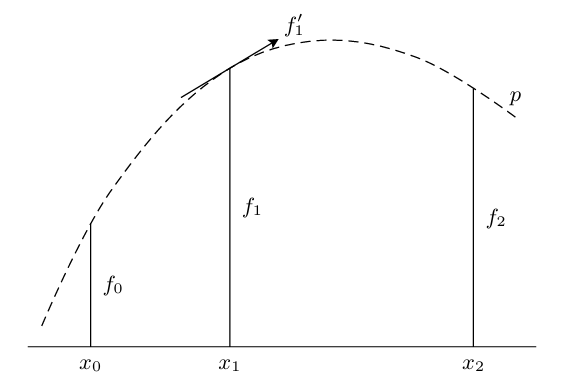
\includegraphics[width=0.75\textwidth]{images/hermite.png}
    \caption{Hermite 插值的例子}
    \label{fig::hermite_divided_difference}
\end{figure}

那么是否可以用 Lagrange 插值的思想来处理呢? 我们补充一个例子:

已知函数 $f(x)$ 在节点 $x_0, x_1, x_2$ 上的函数值 $y_0, y_1, y_2$ 和在 $x_1$ 处的导数值
$m_1$, 即                                                                           
$$
f(x_i) = y_i,\quad i = 0, 1, 2, \qquad f'(x_1) = m_1,
$$                                 
求一个次数不超过 $3$ 的多项式 $P(x)$, 使得                                            
$$
P(x_i) = y_i,\quad i = 0, 1, 2, \qquad P'(x_1) = m_1.
$$  

构造基函数. 设                                                                   
$$
P(x) = y_0 \varphi_0(x) + y_1 \varphi_1(x) + y_2 \varphi_2(x) + m_1 \psi(x)
$$                                 
其中假定 $\varphi_0(x), \varphi_1(x), \varphi_2(x), \psi(x)$ 都是3次多项式.
若它们分别满足下列条件:     
\begin{eqnarray*}                                                                                    
&\varphi_0(x_0)=1, \quad &\varphi_0(x_1)=\varphi_0(x_2)=\varphi'_0(x_1)=0,\\             
&\varphi_1(x_1)=1,\quad &\varphi_1(x_0)=\varphi_1(x_2)=\varphi'_1(x_1)=0,\\             
&\varphi_2(x_2)=1,\quad &\varphi_2(x_0)=\varphi_2(x_1)=\varphi'_2(x_1)=0,\\             
&\psi'(x_1)=1,\quad &\psi(x_0)=\psi(x_1)=\psi(x_2)=0.                                   
\end{eqnarray*}                                                                                      
则上述 $P(x)$ 即为所求.

于是                                                                                     
\begin{eqnarray*}                                                                                            
\varphi_0(x)&=&\frac{(x-x_1)^2(x-x_2)}{(x_0-x_1)^2(x_0-x_2)}\\                                       
\varphi_1(x)&=&(x-x_0)(x-x_2)\Big[\frac{(x_0+x_2-2x_1)}{x_1-x_0)^2(x_1-x_2)^2}(x-x_1)+\frac{1}{(x_1-\
x_0)(x_1-x_2)}\Big]\\                                                                               
\varphi_2(x)&=&\frac{(x-x_0)(x-x_1)^2}{(x_2-x_0)(x_2-x_1)^2}\\                                       
\psi(x)&=&\frac{(x-x_0)(x-x_1)(x-x_2)}{(x_1-x_0)(x_1-x_2)}                                           
\end{eqnarray*}                                                                                                  
得到$P(x)$.

当然, 在实际工作中, 要求得到节点处的精确导数是不太现实的要求. Hermite 插值
更多的用于一些公式的推导.


\subsection{Runge 现象}
% sec 2.7

\begin{example}
    % exp 2.40
    \label{exp::runge}
在定理 \ref{thm::polynomial_interpolation} 中,点 $x_0,x_1,\ldots,x_n$ 往往事先给定,
例如在区间 $[x_0,x_n]$ 上等距分布。随着 $n$ 的增大,插值多项式的次数也随之增大。理想情况下,我们希望
\begin{equation}
    % eq 2.39
    \label{eq::runge}
\forall f\in C[x_0,x_n],\ \forall x\in[x_0,x_n],\qquad
\lim_{n\to+\infty} p_n(f;x)=f(x).
\end{equation}
然而,对于等距节点的多项式插值,这并不成立。著名的 Runge 例子(见图 \ref{fig::runge})展示了在区间端点处的剧烈振荡。
\end{example}

\begin{figure}
    % fig 2.2
    \centering
    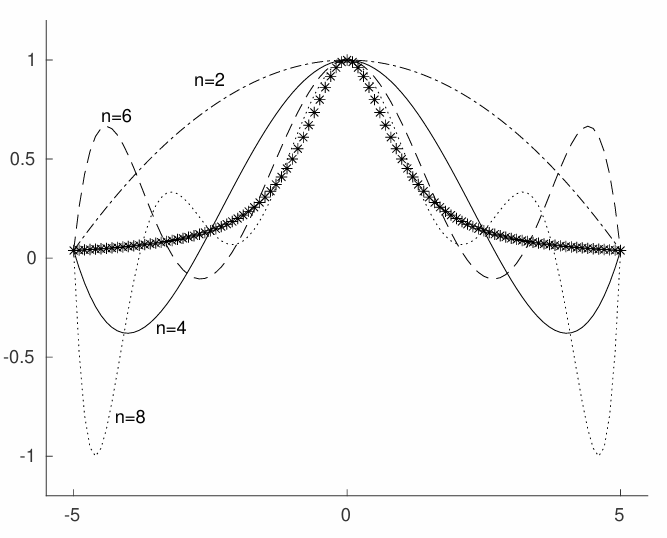
\includegraphics[width=0.75\textwidth]{images/Runge.png}
    \caption{通过在节点 $x_i=-5+10\,\tfrac{i}{n}$($i=0,1,\ldots,n$,$n=2,4,6,8$)上对
$f(x)=\dfrac{1}{1+x^{2}}$ 进行插值而产生的 Runge 现象。}
    \label{fig::runge}
\end{figure}

\begin{remark}
    % remark 2.29
Runge 现象是如何产生的?尽管上图中的误差很大,Cauchy 余项定理仍然成立:
\begin{equation*}
R_n(f;x):=f(x)-p_n(f;x)=\frac{f^{(n+1)}(\xi)}{(n+1)!}\prod_{i=0}^{n}(x-x_i).
\end{equation*}
要理解 Runge 现象,我们提出问题:右端这三个因子中,究竟是哪一个导致了巨大的误差?
显然不是 $(n+1)!$; 也不是 $\prod_{i=0}^{n}(x-x_i)$, 因为我们可以选择使 $x_n-x_0<1$, 
从而每个因子都小于 $1$. 于是罪魁祸首只能是 $f^{(n+1)}(\xi)$.

我们的推理从链式法则开始,它意味着函数 $f(x)=g(x)h(x)$ 的各阶导数中项的数量呈指数增长:
\begin{equation*}
f'=g'h+gh',\qquad
f''=g''h+g'h'+g'h'+gh'',\quad \ldots
\end{equation*}
这种模式仿佛一棵满二叉树,$f^{(n)}$ 中的项数为 $2^{n}$, 且每一项都形如 $g^{(i)}h^{(n+1-i)}$. 
如果这些导数都是有界的(即 $O(1)$),那么随着 $n$ 增加,$f^{(n)}$ 永远不可能超过 $n!$, 因为比值判别法给出
\begin{equation*}
\forall c\in\mathbb{R},\qquad \lim_{n\to+\infty}\frac{c^{n}}{n!}=0.
\end{equation*}
因此,函数 $f$ 必然具有某些特殊性质,使得其高阶导数的增长快于 $n!$.
\end{remark}

\begin{example}
    % exp 2.41
    \label{exp::runge_circle}
有些函数无法被多项式很好地逼近。图 \ref{fig::runge_circle} 中,一条过原点的圆,其半径为 $R$, 圆心位于 $(-R\sin\theta,\; R\cos\theta)$. 当
\begin{equation*}
x\in\bigl(0,\; R-R\sin\theta\bigr)
\end{equation*}
时,该圆弧可以表示为某个函数的图像:
\begin{equation}
    % eq 2.40
    \label{eq::runge_circle}
y=H(x)=R\cos\theta-\sqrt{\,R^{2}-\bigl(x+R\sin\theta\bigr)^{2}\,}.
\end{equation}
$H(x)$ 的阶乘与各阶导数的取值见图 \ref{fig::runge_circle} 中的表。
\end{example}

\begin{figure}
    % fig 2.3
    \centering
    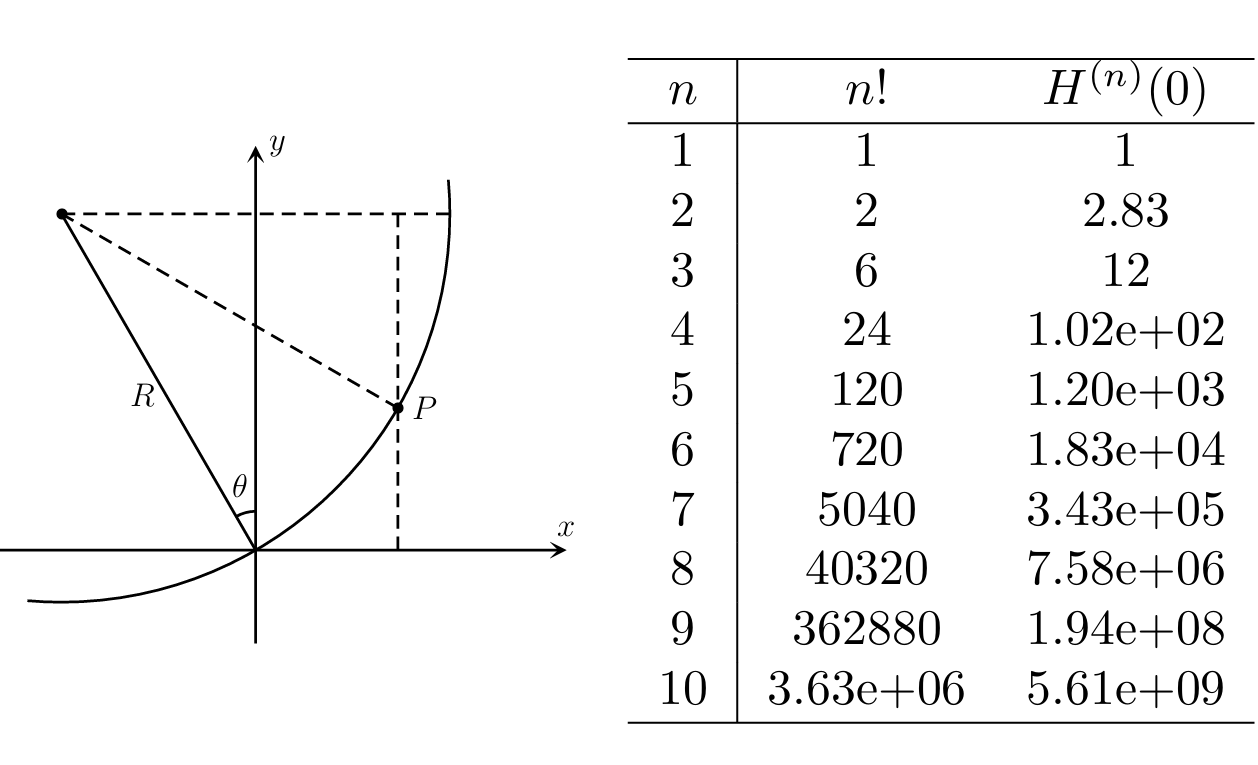
\includegraphics[width=0.75\textwidth]{images/runge_circle.png}
    \caption{用式 (\ref{eq::runge_circle}) 中的函数 $H$ 表示一段局部圆弧。}
    \label{fig::runge_circle}
\end{figure}

\begin{remark}
    % remark 2.30
设 $f:[a,b]\to\mathbb{R}$ 连续,定义
\begin{equation*}
x_i=a+i\,\tfrac{b-a}{n},\qquad i=0,1,\ldots,n,
\end{equation*}
并对每个 $n\in\mathbb{N}^+$ 用这些 $x_i$ 作为插值节点构造多项式插值函数 $p_n(f;x)$. 
理想情况下,我们希望用序列 $(p_n(f))_{n=1}^{\infty}$ 一致逼近 $f$, 即
\begin{align*}
&\forall \varepsilon>0,\ \exists N\in\mathbb{N}^+\ \text{s.t.}\ \forall x\in[a,b],\ \forall n>N, \\
&| p_n(f;x)-f(x) |_{\infty}<\varepsilon.
\end{align*}
然而,由于 Runge 现象,这显然要求过高。于是我们把期望降低为逐点收敛:
\begin{align*}
&\forall \varepsilon>0,\ \forall x\in[a,b],\ \exists N\in\mathbb{N}^+\ \text{s.t.}\ \forall n>N, \\
& |p_n(f;x)-f(x)|_{\infty}<\varepsilon,
\end{align*}
但这同样不成立,因为当 $x_E=\tfrac{1}{2}(x_0+x_1)$ 时,Runge 现象中的误差 $| p_n(f;x)-f(x)|_{\infty} $ 
会随着 $n$ 的增大而增大。该发散由例 \ref{exp::runge_circle} 展示,并在 Trefethen(2013)中有非常好的解释。

总之,在等距网格上使用很高阶的多项式插值并不是逼近所有连续函数的好方法。
\end{remark}

\begin{remark}
    % remark 2.31
我们现在面临一个严肃的问题:待插值的函数通常是固定的,而 $H^{(n)}$ 的大小会随着 $n$ 的增加而迅速增长。
为应对这一问题,我们可以采用分段插值或 Chebyshev 多项式两种方法。
分段插值(见第 2.10 节与第 3 章)的要义是:在越来越多的子区间上使用低次数多项式;
而 Chebyshev 多项式方法的要义是:明智地选择插值点的分布位置。
\end{remark}

下面补充一段内容\textbf{多项式求根}.


\subsection{Chebyshev 多项式}
    % sec 2.8

\begin{remark}
    % remark 2.32
在推论 \ref{cor::cauchy_remainder} 的 Cauchy 余项估计中,若函数 $f$ 通常事先给定,
我们对 $\max\lvert f^{(n+1)}(x)\rvert$ 无能为力。然而,如果我们可以自由选择插值点的位置,
就能进一步减小余项。更具体地说,如何选择 $x_0,x_1,\ldots,x_n$ 来最小化
\begin{equation*}
\max_{x\in[a,b]} \bigl\lvert (x-x_0)(x-x_1)\cdots(x-x_n) \bigr\rvert \, ?
\end{equation*}
满足这一性质的 $x_i$ 正是 Chebyshev 多项式的零点。

这里其实有一个更加一般性的策略,我们知道多项式一般意义上会围绕它的零点振荡,且现在振荡的幅度和插值误差相关。
现在我们希望降低整体误差,但我们不可能消除这种振荡行为,于是一种考虑是,调整插值节点,让振荡变得“均匀”。
Chebyshev 多项式利用欧拉公式和三角函数性质来实现这一点。
\end{remark}

\begin{definition}
    % def 2.42
    \label{def::chebyshev_polynomial}
设 $n\in\mathbb{N}$. 第一类 Chebyshev 多项式是指多项式 $T_n:[-1,1]\to[-1,1]$, 其定义为
\begin{equation}
    % eq 2.41
    \label{eq::chebyshev_polynomial}
T_n(x)=\cos\bigl(n\arccos x\bigr).
\end{equation}
\end{definition}

\begin{remark}
    % rem 2.32
首先,$\lvert T_n(x)\rvert\le 1$. 其次,式 (\ref{eq::chebyshev_polynomial}) 确实定义了一个次数为 $n$ 的多项式。
令 $x=\cos\theta$, 其中 $\theta\in[0,\pi]$. 则
\begin{equation*}
e^{i\theta}=\cos\theta+i\sin\theta
\end{equation*}
从而
\begin{equation*}
\left(e^{i\theta}\right)^{n}=e^{in\theta}=\cos(n\theta)+i\sin(n\theta)=\left(x+i\sqrt{1-x^{2}}\right)^{n}
\end{equation*}
于是
\begin{equation*}
\cos n\theta
= x^{n}+\binom{n}{2}x^{\,n-2}(x^{2}-1)+\cdots ,
\end{equation*}
其中第一行是欧拉公式,最后一行来自二项式定理。前五个 Chebyshev 多项式为
\begin{align*}
T_0(x)&=1,\\
T_1(x)&=x,\\
T_2(x)&=2x^{2}-1,\\
T_3(x)&=4x^{3}-3x,\\
T_4(x)&=8x^{4}-8x^{2}+1.
\end{align*}
除了上述显式公式外,Chebyshev 多项式还可以通过一个递推关系来生成。
\end{remark}

\begin{theorem}
    % thm 2.43
    \label{thm::chebyshev_recurrence}
第一类 Chebyshev 多项式满足如下递推关系:
\begin{equation}
    % eq 2.42
    \label{eq::chebyshev_recurrence}
\forall n\in\mathbb{N}^+,\qquad T_{n+1}(x)=2x\,T_n(x)-T_{n-1}(x).
\end{equation}
\end{theorem}

\begin{proof}
由三角恒等式可得
\begin{align*}
\cos\bigl((n+1)\theta\bigr)&=\cos n\theta \cos\theta-\sin n\theta \sin\theta,\\
\cos\bigl((n-1)\theta\bigr)&=\cos n\theta \cos\theta+\sin n\theta \sin\theta.
\end{align*}
将两式相加并令 $\cos\theta=x$ 即得所需结论。
\end{proof}

\begin{corollary}
    % cor 2.44
    \label{cor::chebyshev_coefficient}
对每个 $n>0$, $T_n$ 中 $x^n$ 的系数为 $2^{\,n-1}$.
\end{corollary}

\begin{proof}
利用上式递推关系以及 $T_1=x$, 用数学归纳法即可证明。
\end{proof}

\begin{remark}
    % remark 2.33
回忆:函数 $f:X\to\mathbb{R}$ 在点 $x^*\in X$ 处具有一个局部极大值,当且仅当
\begin{equation*}
\exists\,\varepsilon>0\ \text{s.t.}\ \forall x\in X,\ d_X(x,x^*)\le \varepsilon \ \Rightarrow\ f(x)\le f(x^*),
\end{equation*}
其中 $(X,d_X)$ 是一个度量空间。
\end{remark}

\begin{theorem}
    % thm 2.45
    \label{thm::chebyshev_zeros_extrema}
$T_n(x)$ 在如下 $n$ 个点处具有单零点:
\begin{equation}
    % eq 2.43
    \label{eq::chebyshev_zeros}
x_k=\cos\!\left(\frac{2k-1}{2n}\pi\right),\qquad k=1,2,\ldots,n.
\end{equation}
当 $x\in[-1,1]$ 且 $n\in\mathbb{N}^+$ 时,$T_n(x)$ 在如下 $n+1$ 个点处取得极值:
\begin{equation}
    % eq 2.44
    \label{eq::chebyshev_extrema}
x_k'=\cos\!\left(\frac{k}{n}\pi\right),\qquad k=0,1,\ldots,n,
\end{equation}
并且在这些点处的取值交替为 $(-1)^k$.
\end{theorem}

\begin{proof}
由 (\ref{eq::chebyshev_polynomial}) 与 (\ref{eq::chebyshev_zeros}) 可得
\begin{equation*}
T_n(x_k)=\cos\!\left(n\arccos\!\bigl(\cos\tfrac{2k-1}{2n}\pi\bigr)\right)
= \cos\!\left(\tfrac{2k-1}{2}\pi\right)=0.
\end{equation*}
对 (\ref{eq::chebyshev_polynomial}) 求导得
\begin{equation*}
T_n'(x)=\frac{n}{\sqrt{1-x^2}}\sin\!\bigl(n\arccos x\bigr).
\end{equation*}
于是每个 $x_k$ 均为单零点,因为
\begin{equation*}
T_n'(x_k)=\frac{n}{\sqrt{1-x_k^2}}\sin\!\left(\tfrac{2k-1}{2}\pi\right)\ne 0.
\end{equation*}
相反地,对任意 $k=1,2,\ldots,n-1$,
\begin{equation*}
T_n'(x_k')=n\Bigl(1-\cos^2\tfrac{k\pi}{n}\Bigr)^{-1/2}\sin(k\pi)=0;
\end{equation*}
并且
\begin{equation*}
T_n''(x)=\frac{n^2\cos\!\bigl(n\arccos(x)\bigr)}{x^2-1}
+\frac{n\,x\,\sin\!\bigl(n\arccos(x)\bigr)}{(1-x^2)^{3/2}},\qquad
T_n''(x_k')\ne 0.
\end{equation*}
因此对 $T_n$ 作 Taylor 展开,得到
\begin{equation*}
T_n(x_k'+\delta)=T_n(x_k')+\frac{1}{2}T_n''(x_k')\delta^2+O(\delta^3),
\end{equation*}
从而 $T_n$ 必在每个 $x_k'$ 处取得局部极值。对任意 $k=0,1,\ldots,n$, 
$T_n(x)$ 在 $x_k'$ 处取极值,因为 $T_n(x_0')=1,\ T_n(x_1')=-1,\ \ldots$, 
且由 (\ref{eq::chebyshev_polynomial}) 知 $\lvert T_n(x)\rvert\le 1$. 
显然这些就是 $T_n(x)$ 在 $[-1,1]$ 上的全部极值点。
\end{proof}

\begin{remark}
    % remark 2.34
可以更为简洁地证明 (\ref{eq::chebyshev_extrema})。由于 $T_n(x)$ 是次数为 $n$ 的多项式,
$T_n'(x)$ 是次数为 $n-1$ 的多项式,至多有 $n-1$ 个互异零点。
易见 $\{x_k'\}_{k=1}^{n-1}$ 正是 $T_n(x)$ 在 $(-1,1)$ 内的 $n-1$ 个互异极值点。
由费马定理知,它们必为 $T_n'(x)$ 的 $n-1$ 个互异零点。
因此,$\{x_k'\}_{k=1}^{n-1}$ 就是 $T_n$ 在 $(-1,1)$ 的全部极值点。结合 $-1$ 与 $1$ 也是 $T_n$ 的极值点即可完成证明。
\end{remark}

\begin{remark}
    % remark 2.35
要理解 Chebyshev 多项式的零点和极值点的位置,可以考虑另一种视角。

根据定理 \ref{thm::chebyshev_zeros_extrema},Chebyshev 多项式的零点等于单位圆上 $2n$ 个等间距点在实轴上的投影。
在图 \ref{fig::chebyshev_zeros_extrema} 中,$n+1$ 个方形标记表示极值点,星号表示单位圆上点 $\exp\!\bigl(i\,\tfrac{2k-1}{2n}\pi\bigr)$, 
它们在水平轴上的投影即为零点。

而从 $T_n$ 的定义不难看出,它的极值点分别是 $-1$ 和 $1$.
\end{remark}

\begin{figure}
    % fig 2.4
    \centering
    \includegraphics[width=0.75\textwidth]{images/chebyshev.png}
    \caption{$n = 4$ 的Chebyshev 多项式的零点与极值点。}
    \label{fig::chebyshev_zeros_extrema}
\end{figure}

\begin{exercise}
    % ex 2.46
编写程序复现实验图 \ref{fig::chebyshev_zeros_extrema}。
\end{exercise}

\begin{remark}
    % remark 2.36
对定义在区间 $[-1,1]$ 上、次数不超过 $n$ 的多项式而言,其零点与极值点的最大个数分别为 $n$ 与 $n+1$. 
如定理 \ref{thm::chebyshev_zeros_extrema} 所证并在上图所示,Chebyshev 多项式同时达到了这两个最大值。
这个事实,结合其三角函数定义,以及 $T_n(x)$ 的首项系数,不难引出了本节的核心结果。
\end{remark}

\begin{theorem}[Chebyshev]
    % thm 2.47
记 $\widetilde{\mathbb{P}}_n$ 为所有首项系数为 $1$、次数为 $n\in\mathbb{N}^+$ 的多项式的集合。则
\begin{equation}
    % eq 2.45
    \label{eq::chebyshev_minimax}
\forall p\in\widetilde{\mathbb{P}}_n,\qquad
\max_{x\in[-1,1]}\left|\frac{T_n(x)}{2^{n-1}}\right|
\le \max_{x\in[-1,1]} |p(x)|.
\end{equation}
\end{theorem}

\begin{proof}
由定理 \ref{thm::chebyshev_zeros_extrema},$T_n(x)$ 在式(\ref{eq::chebyshev_extrema})
中的点 $x_k'$ 处取得 $n+1$ 个极值。设上述不等式不成立,则定理 \ref{thm::chebyshev_zeros_extrema} 蕴含
\begin{equation}
    % eq 2.46
    \label{eq::chebyshev_contradiction}
\exists\,p\in\widetilde{\mathbb{P}}_n\ \text{s.t.}\ 
\max_{x\in[-1,1]}|p(x)|<\frac{1}{2^{n-1}}.
\end{equation}
考虑多项式 $Q(x)=\frac{1}{2^{n-1}}T_n(x)-p(x)$. 则
\begin{equation*}
Q(x_k')=\frac{(-1)^k}{2^{n-1}}-p(x_k'),\qquad k=0,1,\ldots,n.
\end{equation*}
由上式知,$Q(x)$ 在这 $n+1$ 个点处符号交替。因此 $Q(x)$ 必有 $n$ 个零点。
然而按构造,$Q(x)$ 的次数至多为 $n-1$. 于是 $Q(x)\equiv 0$ 且 $p(x)=\frac{1}{2^{n-1}}T_n(x)$, 从而
$\max |p(x)|=\frac{1}{2^{n-1}}$. 这与前述不等式矛盾。
\end{proof}

\begin{corollary}
    % cor 2.48
对任意 $n\in\mathbb{N}^+$, 有
\begin{equation}
    % eq 2.47
    \label{eq::chebyshev_lower_bound}
\max_{x\in[-1,1]}\bigl|x^n+a_1 x^{n-1}+\cdots+a_n\bigr|\ge \frac{1}{2^{n-1}}.
\end{equation}
\end{corollary}

\begin{corollary}
    % cor 2.49
若对函数 $f$ 在定理 \ref{thm::chebyshev_zeros_extrema} 中 $T_{n+1}(x)$ 的 $n+1$ 个零点上进行多项式插值,
则定理 \ref{thm::cauchy_remainder} 的 Cauchy 余项满足
\begin{equation}
    % eq 2.48
    \label{eq::chebyshev_remainder}
\lvert R_n(f;x)\rvert \le \frac{1}{2^n (n+1)!}\,
\max_{x\in[-1,1]}\bigl|f^{(n+1)}(x)\bigr|.
\end{equation}
\end{corollary}

\begin{proof}
由定理 \ref{thm::cauchy_remainder}、推论 \ref{cor::chebyshev_coefficient} 与定理 \ref{thm::chebyshev_zeros_extrema} 得
\begin{equation*}
\lvert R_n(f;x)\rvert
=\frac{\lvert f^{(n+1)}(\xi)\rvert}{(n+1)!}\left|\prod_{i=0}^{n}(x-x_i)\right|
=\frac{\lvert f^{(n+1)}(\xi)\rvert}{2^n (n+1)!}\,|T_{n+1}|.
\end{equation*}
由定义 \ref{def::chebyshev_polynomial} 可知 $|T_{n+1}|\le 1$, 从而结论成立。
\end{proof}

\begin{remark*}
    至此,回答了本节开头提出的问题。Chebyshev 多项式的零点使得插值多项式的误差最小化。
这组节点是所谓的“最好”的插值节点。但是注意,我们插值的问题动机是已知一些节点的函数值,
希望估计非节点处的函数值。因此这些已知节点往往来自问题和需求,不能由我们决定。除非,
我们的问题契约已经变为通过插值,给出一个已知函数 $f$ 的近似多项式 $p_n(f)$.
在这种情况下,Chebyshev 多项式的零点是一个很好的选择。但这种情况下,
实际问题已经从数据拟合变为函数逼近。

那么一个自然的问题是,是否任何连续函数都能被多项式一致逼近?要回答这个问题,首先要考虑一致收敛是在什么范数的意义下。
可以证明,在 $2$-范数下,Chebyshev 多项式的零点插值多项式序列确实一致收敛于任何连续函数,这种逼近是所谓的最佳平方逼近。
然而,在 $\infty$-范数下,这并不成立。但最大模意义下我们可以构建另一种多项式逼近方法,也即最佳一致逼近。
这种插值多项式的构造见下面一节。仍然是从基函数开始构建。注意,这里我们实际上已经放弃了插值的要求,我们得到的多项式,
并不是插值多项式,因为它已经没有所谓的插值节点了。
\end{remark*}

\subsection{Bernstein 多项式}
    % subsec 2.9

\begin{definition}
    % def 2.50
    \label{def::bernstein_basis}
次数为 $n\in\mathbb{N}^+$、相对于单位区间 $[0,1]$ 的 Bernstein 基多项式定义为
\begin{equation}
    % eq 2.49
    \label{eq::bernstein_basis_def}
\forall k=0,1,\ldots,n,\qquad
b_{n,k}(t):=\binom{n}{k} t^{k}(1-t)^{n-k},
\end{equation}
并约定当整数 $k$ 取其他值时,$b_{n,k}(t)=0$.
\end{definition}

\begin{example}
    % ex 2.51
当 $n=3$ 时,Bernstein 基多项式为
$t^{3},\ 3t^{2}(1-t),\ 3t(1-t)^{2},\ (1-t)^{3}$.
\end{example}

\begin{definition}
    % def 2.52
Bernstein 多项式是 Bernstein 基多项式的线性组合,即 $\sum_{k=0}^{n}\beta_{k} b_{n,k}$,
其中系数称为 Bernstein 系数或 Bézier 系数。
\end{definition}

\begin{remark*}
Bernstein 多项式最初由 Bernstein(1912)引入,它有一些非常好的性质。
\end{remark*}

\begin{lemma}
    % lem 2.53
一个 Bernstein 基多项式总可以表示为更高次数 Bernstein 基多项式的线性组合:
\begin{equation}
    % eq 2.50
    \label{eq::bernstein_degree_elev}
b_{n-1,k}(t)=\frac{n-k}{n}\, b_{n,k}(t)+\frac{k+1}{n}\, b_{n,k+1}(t).
\end{equation}
\end{lemma}

\begin{proof}
这由定义 \eqref{eq::bernstein_basis_def} 直接推出。
\end{proof}

\begin{lemma}
    % lem 2.54
Bernstein 基多项式的导数是两个更低次数 Bernstein 基多项式的线性组合,即
\begin{equation}
    % eq 2.51
    \label{eq::bernstein_derivative}
b'_{n,k}(t)=n\, b_{n-1,k-1}(t)-n\, b_{n-1,k}(t).
\end{equation}
\end{lemma}

\begin{proof}
这由定义 \eqref{eq::bernstein_basis_def} 直接推出。
\end{proof}

\begin{lemma}
    % lem 2.55
Bernstein 基多项式的积分只与其次数有关,即
\begin{equation}
    % eq 2.52
    \label{eq::bernstein_integral}
\forall k=0,1,\ldots,n,\qquad \int_{0}^{1} b_{n,k}(t)\,\mathrm{d}t=\frac{1}{n+1}.
\end{equation}
\end{lemma}

\begin{proof}
由式 \eqref{eq::bernstein_basis_def} 并配合分部积分即可得到。
\end{proof}

\begin{lemma}
    % lem 2.56
    \label{lem::bernstein_basis}
次数为 $n$ 的 Bernstein 基多项式构成 $\mathbb{P}_n$ 的一组基,其中 $\mathbb{P}_n$ 表示次数不超过 $n$ 的全部多项式的向量空间。
\end{lemma}

\begin{proof}
由定义 \eqref{eq::bernstein_basis_def},可写
\begin{equation*}
b_{n,k}(t)=\sum_{j=k}^{n} a_{k,j} t^{j},
\end{equation*}
因而有
\begin{equation*}
\begin{bmatrix}
b_{n,0}(t)\\
b_{n,1}(t)\\
b_{n,2}(t)\\
\vdots\\
b_{n,n}(t)
\end{bmatrix}
=
\begin{bmatrix}
a_{0,0} & a_{0,1} & a_{0,2} & \cdots & a_{0,n}\\
0 & a_{1,1} & a_{1,2} & \cdots & a_{1,n}\\
0 & 0 & a_{2,2} & \cdots & a_{2,n}\\
\vdots & \vdots & \vdots & \ddots & \vdots\\
0 & 0 & 0 & \cdots & a_{n,n}
\end{bmatrix}
\begin{bmatrix}
1\\ t\\ t^{2}\\ \vdots\\ t^{n}
\end{bmatrix},
\end{equation*}
其中该矩阵为上三角矩阵,且对角线元 $a_{k,k}=\binom{n}{k}\ne 0$. 其余结论由单项式构成 $\mathbb{P}_n$ 的一组基立即得到。
\end{proof}

\begin{lemma}
    % lem 2.57
Bernstein 基多项式满足
\begin{subequations}
    \label{eq::bern_2_53}
\begin{equation}
\label{eq::bern_2_53a}
\forall k=0,1,\ldots,n,\ \forall t\in(0,1),\qquad b_{n,k}(t)>0,
\end{equation}
\begin{equation}
\label{eq::bern_2_53b}
\sum_{k=0}^{n} b_{n,k}(t)=1,
\end{equation}
\begin{equation}
\label{eq::bern_2_53c}
\sum_{k=0}^{n} k\, b_{n,k}(t)=n t,
\end{equation}
\begin{equation}
\label{eq::bern_2_53d}
\sum_{k=0}^{n} k^{2} b_{n,k}(t)=n(n-1)t^{2}+n t,
\end{equation}
\begin{equation}
\label{eq::bern_2_53e}
\sum_{k=0}^{n} (k-n t)^{2} b_{n,k}(t)=n t(1-t).
\end{equation}
\end{subequations}
\end{lemma}

\begin{proof}
\eqref{eq::bern_2_53a} 由式(\ref{eq::bernstein_basis_def})得到;\eqref{eq::bern_2_53b} 则由二项式定理
\begin{equation}
    % eq 2.54
\sum_{k=0}^{n}\binom{n}{k} t^{k} s^{\,n-k}=(t+s)^{n}.
\end{equation}
对上式关于 $t$ 求导并两边同乘以 $t$, 得到
\begin{equation*}
(\ast):\qquad \sum_{k=0}^{n} k \binom{n}{k} t^{k} s^{\,n-k}=n t (t+s)^{n-1}.
\end{equation*}
令 $s=1-t$ 即得 \eqref{eq::bern_2_53c};再次对 $(\ast)$ 关于 $t$ 求导并两边同乘以 $t$, 并配合
\eqref{eq::bern_2_53b} 与 \eqref{eq::bern_2_53c} 化简,得到 \eqref{eq::bern_2_53d};
将 $s=1-t$ 代入 \eqref{eq::bern_2_53d},再用 $-2 n t(\ast)+n^{2} t^{2}(t+s)^{n}$ 化简,即得 \eqref{eq::bern_2_53e}。
\end{proof}

\begin{remark}
    % remark 2.37
由 \eqref{eq::bern_2_53a} 与 \eqref{eq::bern_2_53b} 可知,Bernstein 基多项式构成定义 D.152 
意义下的统一分解(partition of unity)。这在数值分析与计算中非常有用,并将在第 3 章再次出现。
\end{remark}

\begin{definition}
    % def 2.58
    \label{def::bernstein_polynomial}
函数 $f\in\mathcal{C}[0,1]$ 的第 $n$ 个 Bernstein 多项式定义为
\begin{equation}
    % eq 2.55
    \label{eq::bernstein_polynomial}
(B_n f)(t):=\sum_{k=0}^{n} f\!\left(\frac{k}{n}\right) b_{n,k}(t),
\end{equation}
其中 $b_{n,k}$ 为式(\ref{eq::bernstein_basis_def})中的 Bernstein 基多项式。
\end{definition}

\begin{remark*}
Bernstein 多项式不是插值多项式,因为它并不满足插值条件 
$$
p_n(f;x_i)=f(x_i).
$$    
\end{remark*}

\begin{theorem}[Weierstrass 逼近定理]
    % thm 2.59
任意连续函数 $f:[a,b]\to\mathbb{R}$ 都可以被一列多项式以任意精度一致逼近,即
\begin{equation}
    % eq 2.56
    \label{eq::weierstrass_theorem}
\forall f\in\mathcal{C}[a,b],\ \forall \epsilon>0,\ \exists N\in\mathbb{N}^+\ \text{s.t.}\ \forall n>N,\ 
\exists p_n\in \mathbb{P}_n\ \text{s.t.}\ \forall x\in[a,b],\ |p_n(x)-f(x)|<\epsilon.
%\label{eq::weierstrass_statement}
\end{equation}
\end{theorem}

\begin{proof}
不失一般性,设 $a=0,\ b=1$. 令 $p_n=B_n f$, 参见式(\ref{eq::bernstein_polynomial})。
对任意 $\epsilon>0$, 存在 $\delta>0$ 与 $n\in\mathbb{N}^+$, 使得
\begin{align*}
\bigl|(B_n f)(t)-f(t)\bigr|
&=\left|(B_n f)(t)-f(t)\sum_{k=0}^{n} b_{n,k}(t)\right| \nonumber\\
&\le \sum_{k=0}^{n}\left| f\!\left(\frac{k}{n}\right)-f(t)\right| b_{n,k}(t) \nonumber\\
&=\left(\sum_{k:\,\left|\frac{k}{n}-t\right|<\delta}\ +\ \sum_{k:\,\left|\frac{k}{n}-t\right|\ge \delta}\right)
\left| f\!\left(\frac{k}{n}\right)-f(t)\right| b_{n,k}(t) \nonumber\\
&\le \sup_{|t-s|\le \delta} |f(t)-f(s)|\ +\ \frac{\lVert f\rVert_\infty}{2n\delta^{2}} \nonumber\\
&\le \frac{\epsilon}{2}+\frac{\epsilon}{2}=\epsilon,
\end{align*}
其中第一步来自式(\ref{eq::bernstein_polynomial})与三角不等式;第二行中情形 $|k-nt|<n\delta$ 由
\eqref{eq::bern_2_53a} 与 \eqref{eq::bern_2_53b} 得到,情形 $|k-nt|\ge n\delta$ 则由
\eqref{eq::bern_2_53e} 与
\begin{equation*}
\sum_{k:\, \left|\frac{k}{n}-t\right|\ge \delta} b_{n,k}(t)
\le \sum_{k:\, \left|\frac{k}{n}-t\right|\ge \delta} b_{n,k}(t)\frac{(k-nt)^2}{\delta^{2} n^{2}}
\le \sum_{k=0}^{n} b_{n,k}(t)\frac{(k-nt)^2}{\delta^{2} n^{2}}
= \frac{t(1-t)}{n\delta^{2}}\le \frac{1}{4n\delta^{2}}
\end{equation*}
而最后一个不等式来自 $f$ 的一致连续性(参见定理 C.79)以及选择 $n>\lVert f\rVert_\infty/(\epsilon\delta^{2})$。
\end{proof}

\begin{remark}
    % remark 2.39
这个定理一般不被看作是一个数值计算的结果,因为其收敛速度通常很慢。它更多的是理论意义上证明了在无穷范数下的连续函数空间中,
多项式空间是稠密的。
    
Weierstrass 逼近定理在理论上“挽救”了 Runge 现象,而后者可由 Bernstein 多项式来实现逼近。
然而,收敛可能非常缓慢。就 Chebyshev 多项式而言,已有结果(见 Natanson, 1965, p. 43)表明,
存在函数 $f\in\mathcal{C}[-1,1]$, 使得当 $n\to\infty$ 时,$f$ 的 Chebyshev 多项式插值在区间 $[-1,1]$ 的所有点上都发散。
这与 Chebyshev 多项式的 Lebesgue 常数呈 $\log(n)$ 发散这一事实一致;
参见 Trefethen, 2013, p. 115。幸运的是,可以证明 Chebyshev 多项式插值在某个 $2$-范数意义下是收敛的;
见 Mason and Handscomb, 2003, p. 158。
\end{remark}

\begin{remark}
    % remark 2.40
Bernstein 基多项式非常有用,并且可以直接推广到更高维情形。令 $T$ 为一个非退化三角形,
其顶点为 $v_i=(x_i,y_i)\in\mathbb{R}^2$. 则任意 $v\in\mathbb{R}^2$ 都可以唯一表示为
\begin{equation*}
v(x,y)=b_1(x,y)v_1+b_2(x,y)v_2+b_3(x,y)v_3,
\end{equation*}
其中重心坐标 $b_i$ 满足
\begin{equation*}
\forall v(x,y)\in\mathbb{R}^2,\qquad b_1(x,y)+b_2(x,y)+b_3(x,y)=1.
\end{equation*}
相对于三角形 $T$ 的次数为 $n$ 的 Bernstein 基多项式为
\begin{equation*}
B^{n}_{ijk}:=\frac{n!}{i!\,j!\,k!}\, b_1^{\,i} b_2^{\,j} b_3^{\,k}.
\end{equation*}
更多细节见 Lai and Schumaker (2007)。
\end{remark}

\begin{remark}
    % remark 2.41
定义函数 $f$ 的全变差为其导数(以分布意义)的 $1$-范数。若 $f$ 的第 $\nu$ 阶导数具有有界变差 $V$, 
则 $f$ 的 Chebyshev 系数满足上界
\begin{equation*}
2\pi^{-1} V (k-\nu)^{-\nu-1}.
\end{equation*}
当 $\nu\ge 1$ 时,可推出 $f$ 的 $n$ 次 Chebyshev 插值的精度为 $O(V n^{-\nu})$;参见 Trefethen (2013), 第 7 章。
\end{remark}

\begin{remark}
    % remark 2.42
函数 $f\in\mathcal{C}[-1,1]$ 的最佳多项式逼近 $p_n$ 当 $n\to\infty$ 时以几何速度收敛
(即存在常数 $\rho>1$ 与 $M$, 依赖于 $f$ 以及 $|f(x)|\le M$, 使得
$\lVert p_n-f\rVert \le \dfrac{M}{\rho^{n}(\rho-1)}$),
当且仅当 $f$ 为解析函数;见 Trefethen (2013), 第 8 章。
因此,$f\in\mathcal{C}[-1,1]$ 越光滑,其最佳逼近收敛得越快。
\end{remark}

\subsection{Hermite 样条}
    % subsec 2.10

\begin{remark*}
    毕竟一个连续函数,同时避免 Runge 现象的另一个更加常用的策略是使用分段多项式插值。
即将目标区间划分为若干子区间,在每个子区间上使用低次多项式插值。最简单的例子是分段线性插值。
如果希望增加插值多项式的光滑性,可以使用分段 Hermite 插值。
\end{remark*}    

\subsubsection{三次 Hermite 样条}
% subsubsec 2.10.1

\begin{definition}
    % def 2.60
    \label{def::cubic_hermite_spline}
三次 Hermite 样条(cubic Hermite spline 或 cubic Hermite interpolator)是由分段三次多项式组成的 $C^1$ 函数,
用以在插值点处给定函数值与导数值的 Hermite 插值问题。
\end{definition}

\begin{lemma}
    % lem 2.61
    \label{lem::cubic_hermite_spline}
考虑 Hermite 插值问题:在点 $x_i$($i=0,1,\ldots,n$ 且对任意 $j=0,1,\ldots,n-1$ 有 $x_j<x_{j+1}$)
处给定函数值 $f_i$ 与导数值 $f_i'$. 相应的三次 Hermite 样条 $p_f$ 属于 $C^1([x_0,x_n])$, 并在区间 $[x_j,x_{j+1}]$ 上由下式给出
\begin{subequations}
    \label{eq::hermite_257}
\begin{equation}
    \label{eq::hermite_257a}
p_f(x)\big|_{[x_j,x_{j+1}]}=:p_j(x)=\sum_{k=0}^{3}\beta_k\, b_{3,k}\!\left(\frac{x-x_j}{x_{j+1}-x_j}\right),
\end{equation}
\begin{equation}
    \label{eq::hermite_257b}
\beta_0=f_j,\qquad \beta_1=f_j+\frac{1}{3}f_j'(x_{j+1}-x_j);
\end{equation}
\begin{equation}
    \label{eq::hermite_257c}
\beta_3=f_{j+1},\qquad \beta_2=f_{j+1}-\frac{1}{3}f_{j+1}'(x_{j+1}-x_j),
\end{equation}
\end{subequations}
其中 $b_{3,k}$ 为定义 \ref{def::bernstein_basis} 中次数为 $3$ 的第 $k$ 个 Bernstein 基多项式。
\end{lemma}

\begin{proof}
由 \eqref{eq::hermite_257a} 可直接验证 $p_j(x)$ 满足插值条件
\begin{equation*}
p_j(x_j)=f_j,\quad p_j(x_{j+1})=f_{j+1};\qquad
p_j'(x_j)=f_j',\quad p_j'(x_{j+1})=f_{j+1}'
\end{equation*}
于区间 $[x_j,x_{j+1}]$ 上。由定义 \ref{def::hermite_interpolation} 与 \ref{def::cubic_hermite_spline} 可知,
$p_f$ 的确是三次 Hermite 样条且属于 $C^1$. 另一方面,每个区间上的四个插值条件唯一地确定 $p_j$, 
因为引理 \ref{lem::bernstein_basis} 表明 $\{b_{3,k}:k=0,1,2,3\}$ 是 $\mathbb{P}_3$ 的一组基,
并且坐标变换 $x\mapsto \dfrac{x-x_j}{x_{j+1}-x_j}$ 是双射。
\end{proof}

\begin{remark*}
构建逐段三次 Hermite 样条的另一个算法是使用 Newton 形式的插值多项式。    
\end{remark*}

\begin{remark}
    % remark 2.43
引理 \ref{lem::cubic_hermite_spline} 提供了一种应对 Runge 现象的方法:
采用固定多项式次数、逐渐增加区间数目的分段多项式插值。
三次 Hermite 样条中的每个三次多项式都可以通过式(\ref{eq::hermite_257})显式计算,
因此仅具有 $C^1$ 连续性。若要使这些三次多项式达到 $C^2$ 连续性,需要将所有区间的信息装配为一个线性方程组,
其解给出样条;参见第 \ref{sec::pp_spline} 节。总而言之,引理 \ref{lem::cubic_hermite_spline} 
所得样条是显式计算、仅为 $C^1$ 或属于 $\mathbb{S}_3^{1}$(参见定义 \ref{def::spline_space});
而定理 \ref{thm::exist_unique_cubic_splines} 中的样条必须通过隐式方式计算,
并且可以达到 $C^2$ 或属于 $\mathbb{S}_3^{2}$.
\end{remark}

\subsubsection{曲线:最基础}
% subsubsec 2.10.2

\begin{definition}
    % def 2.62
(开)曲线是某个连续映射 $\gamma:(\alpha,\beta)\to\mathbb{R}^D$ 的像,
其中 $-\infty\le \alpha<\beta\le +\infty$. 若映射 $\gamma$ 为单射,则称其为简单曲线。
\end{definition}

\begin{remark*}
    注意这个曲线可以是高维的。即曲线的参数化。
\end{remark*}

\begin{definition}
    % def 2.63
曲线 $\gamma$ 的切向量是它的一阶导数
\begin{equation}
    % eq 2.58
\gamma' := \frac{\mathrm{d}\gamma}{\mathrm{d}t},
\end{equation}
而 $\gamma$ 的单位切向量,记为 $\mathbf{t}$, 是其切向量的单位化。
\end{definition}

\begin{definition}
    % def 2.64
单位速度曲线是指其切向量在每一点都具有单位长度的曲线。
\end{definition}

\begin{definition}
    % def 2.65
若 $\gamma(t_0)$ 处的导数 $t(t_0)$ 存在且 $t(t_0)\ne 0$, 
则称点 $\gamma(t_0)$ 为曲线 $\gamma$ 的正则点;若曲线的所有点都是正则点,则称该曲线为正则的。
\end{definition}

\begin{definition}
    % def 2.66
闭曲线是连续映射 $\hat\gamma:[0,1]\to\mathbb{R}^2$ 的像,
并满足 $\hat\gamma(0)=\hat\gamma(1)$. 如果 $\hat\gamma$ 在 $[0,1)$ 的限制进一步为单射,
则该闭曲线称为简单闭曲线或 Jordan 曲线。
\end{definition}

\begin{definition}
    % def 2.67
曲线的带符号单位法向量,记为 $\mathbf{n}_s$, 是将其单位切向量逆时针旋转 $\tfrac{\pi}{2}$ 所得到的单位向量。
\end{definition}

\begin{definition}
    % def 2.68
单位速度曲线 $\gamma$ 的带符号曲率定义为 $\kappa_s := \gamma''\cdot \mathbf{n}_s$.
\end{definition}

\begin{remark}
    % remark 2.44
由隐函数定理 D.121,平面曲线 $\hat\gamma$ 在一个正则点 $p$ 的充分小的局部弧段,总可以重新参数化为
\begin{equation*}
(\ast):\quad \gamma(\xi)=(\xi,\,H(\xi)),
\end{equation*}
其中 $H:\mathbb{R}\to\mathbb{R}$ 称为与参数 $\xi$ 相关联的 $\gamma$ 的高度函数,
且轴 $\xi$ 要么水平要么竖直,即 $\xi=+x$、$\xi=-x$、$\xi=+y$ 或 $\xi=-y$. 见例 \ref{exp::runge_circle}。

$\kappa_s$ 的符号指示单位切向量在局部是逆时针($\kappa_s>0$)还是顺时针($\kappa_s<0$)旋转。
对于形如 $(\ast)$ 的正则局部弧段,其带符号曲率可表示为
\begin{equation*}
\kappa_s=\frac{H''}{\bigl(1+(H')^{2}\bigr)^{3/2}},
\end{equation*}
其中另一条局部坐标轴 $\eta=H(\xi)$ 是通过将 $\xi$ 轴逆时针旋转 $\tfrac{\pi}{2}$ 得到的。
\end{remark}


\subsubsection{Bézier 曲线}
% subsubsec 2.10.3

\begin{definition}
    % def 2.69
    \label{def::bezier_curve}
给定 $\mathbb{R}^D$ 中 $n+1$ 个互异点 $\mathbf{q}_0,\mathbf{q}_1,\ldots,\mathbf{q}_n$, 
其 Bézier 曲线 $\mathbf{B}:[0,1]\to\mathbb{R}^D$ 定义为
\begin{equation}
    % eq 2.59
    \label{eq::bezier_curve}
\mathbf{B}(t):=\sum_{k=0}^{n}\mathbf{q}_k\, b_{n,k}(t),
\end{equation}
其中 $n\in\mathbb{N}^+$, $b_{n,k}$ 为定义 \ref{def::bernstein_basis} 中次数为 $n$ 的第 $k$ 个 Bernstein 基多项式,
这些点 $\mathbf{q}_k$ 称为 Bézier 曲线的控制点。
\end{definition}

\begin{example}
    % ex 2.70
一次 Bézier 曲线为线段;也即,两点确定的一条 Bézier 曲线。二次 Bézier 曲线由三个互异点确定,而三次 Bézier 曲线由四个互异点确定。
\end{example}

\begin{lemma}
    % lem 2.71
    \label{lem::convex_combination}
设两两不同的点 $\mathbf{p}_i\in W\subset\mathbb{R}^n$, 其中 $i=1,\ldots,m$ 且 $m\ge 2$. 
则任一点 $\sum_{i=1}^{m}\lambda_i \mathbf{p}_i$, 
当满足 $\sum_{i=1}^{m}\lambda_i=1$ 且 $\lambda_i\in[0,1]$ 时,属于 $W$ 的凸包。
\end{lemma}

\begin{proof}
当 $m=2$ 时由定义 \ref{def::convex_set} 直接成立。对归纳步,有
\begin{equation*}
\sum_{i=1}^{m}\lambda_i \mathbf{p}_i=\lambda_m \mathbf{p}_m+(1-\lambda_m)\,\mathbf{q}_m,
\end{equation*}
其中 $\mathbf{q}_m:=\sum_{i=1}^{m-1}\frac{\lambda_i}{1-\lambda_m}\mathbf{p}_i$. 
根据归纳假设,$\mathbf{q}_m$ 属于 $W$ 的凸包。于是证明可由归纳基完成。
\end{proof}

\begin{lemma}
    % lem 2.72
由 $n+1$ 个互异点确定的 Bézier 曲线包含于这些点的凸包之内。
\end{lemma}

\begin{proof}
此结论由引理 \ref{lem::convex_combination}、式(\ref{eq::bern_2_53a})、(\ref{eq::bern_2_53b})
以及定义 \ref{def::convex_set} 与 \ref{def::bezier_curve} 推出。
\end{proof}

\begin{lemma}
    % lem 2.73
    \label{lem::bezier_endpoints}
次数为 $n$ 的 Bézier 曲线满足
\begin{subequations}
    \label{eq::bezier_endpoints}
\begin{equation}
\mathbf{B}(0)=\mathbf{q}_0,\qquad \mathbf{B}'(0)=n(\mathbf{q}_1-\mathbf{q}_0);
\end{equation}
\begin{equation}
\mathbf{B}(1)=\mathbf{q}_n,\qquad \mathbf{B}'(1)=n(\mathbf{q}_n-\mathbf{q}_{n-1}).
\end{equation}
\end{subequations}
\end{lemma}

\begin{proof}
将式 (\ref{eq::bezier_curve}) 改写为
\begin{equation*}
\mathbf{B}(t)=\mathbf{q}_n t^{n}+\mathbf{q}_0(1-t)^{n}+\sum_{k=1}^{n-1}\mathbf{q}_k \binom{n}{k} t^{k}(1-t)^{n-k},
\end{equation*}
从而得到 (\ref{eq::bezier_endpoints}) 中的第一组等式;并且
\begin{align*}
\mathbf{B}'(t)
&=n\mathbf{q}_n t^{n-1}-n\mathbf{q}_0(1-t)^{n-1} \nonumber\\
&\quad+\sum_{k=1}^{n-1}\mathbf{q}_k \binom{n}{k}\Bigl[k t^{k-1}(1-t)^{n-k}-(n-k)t^{k}(1-t)^{n-k-1}\Bigr],
\end{align*}
据此可得第二组等式。
\end{proof}

\begin{remark}
    % remark 2.45
由引理 \ref{lem::bezier_endpoints},Bézier 曲线的首尾两个控制点在曲线上。
同时,前两个控制点和后两个控制点分别确定曲线起点与终点处的切向量。
\end{remark}

\begin{algorithm}
    % alg 2.74
(基于三次 Bézier 曲线的曲线拟合)给定切向量 $\gamma'$ 的曲线 $\gamma:(0,1)\to\mathbb{R}^{D}$ 可按如下步骤由三次 Bézier 曲线近似:
\begin{enumerate}
\item 选择 $m+1$ 个相邻的标记点 $\mathbf{p}_0,\ldots,\mathbf{p}_m$ 于 $\gamma$ 上,并在这些标记点处计算切向量。
\item 对每个 $j=0,\ldots,m-1$,计算
\begin{equation*}
\mathbf{q}_0:=\mathbf{p}_j,\qquad
\mathbf{q}_1:=\tfrac{1}{3}\gamma'(\mathbf{p}_j)+\mathbf{p}_j,\qquad
\mathbf{q}_2:=\mathbf{p}_{j+1}-\tfrac{1}{3}\gamma'(\mathbf{p}_j),\qquad
\mathbf{q}_3:=\mathbf{p}_{j+1},
\end{equation*}
并由这些 $\mathbf{q}_j$ 确定一个三次 Bézier 曲线(式 \ref{eq::bezier_curve})。
\item 将这 $m$ 条三次 Bézier 曲线连接起来。
\end{enumerate}
\end{algorithm}

\begin{remark}
    % remark 2.46
由于三次 Bézier 曲线的每个坐标函数都是三次 Hermite 样条,定理 \ref{thm::hermite_remainder} 
蕴含所拟合的三次 Bézier 曲线在相邻标记点最大间距意义下具有四阶精度。

Bézier 曲线提供了一种“手绘”分段曲线表示方法,在计算机图形学软件中有广泛应用。
\end{remark}

\section{样条}
% sec 3

\begin{remark}
    % remark 3.1
正如上一章所讨论的,在等距节点上进行高次数多项式插值会因宽幅振荡而表现不佳,
这由 Runge 现象所示。除了 Chebyshev 多项式之外,
本章中的样条函数构成了实现多项式插值快速收敛的另一种方法。
历史上,样条函数有两种形式:分段多项式(PP)形式便于构造且适合误差分析,
而 B 形式则具有诸如递归构造、局部支撑以及与单位分割的联系等优点。
由定理 \ref{thm::exist_unique_cubic_splines} 知,$C^2$ 的三次样条是唯一的,因此其 PP 形式与 B 形式表示同一个函数。
\end{remark}

\begin{remark}
    % remark 3.2
样条(spline)是一条由弹性材料制成的长条,
在若干点处被固定;该长条在这些固定点的约束下松弛,
形成一条通过这些固定点的光滑曲线,从而将该曲线转移到另一种材料上;
见图 \ref{fig::spline_example}。“样条函数”这一术语最早由 Schoenberg 于 1946 年提出,
用以指代具有与上述机械装置相似性质的分段多项式。
\end{remark}

\begin{remark*}
    绘制曲线是工业制造和设计中的一个重要问题。之前我们已经讨论了 Bézier 曲线,
它们在计算机图形学中有广泛应用。样条函数则更加古老。Spline 装置最初用于船舶设计,
而这个词的原意就是柳木条。在东方,我们主要使用竹条来绘制曲线,
而样这个词来源于放样,或者样式。本质上就是建筑设计和模型制作。比如清代故宫建筑,
主要由一个雷姓世家负责设计和施工,行业内称其为“样式雷”。
\end{remark*}

\begin{figure}
\centering
% 图 3.1 说明
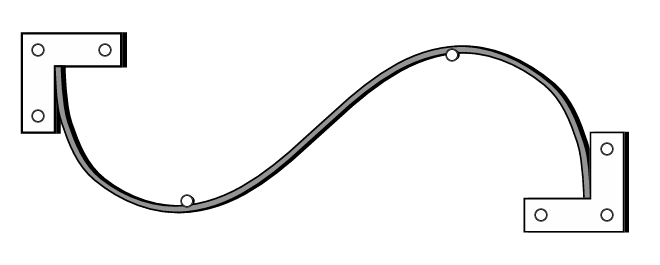
\includegraphics[width=0.6\textwidth]{images/spline.png}
\caption{一个样条示例。L 形支架与圆圈表示固定装置,
阴影加粗的曲线为在这些固定条件下弯曲的木条。}
\label{fig::spline_example}
\end{figure}

\begin{definition}
    % def 3.1
    \label{def::spline_space}
给定非负整数 $n,k$, 以及将区间 $[a,b]$ 划分开的严格递增序列 $(x_i)_{i=1}^{N}$, 
即
\begin{equation}
    % eq 3.1
    \label{eq::partition}
a=x_1<x_2<\cdots<x_N=b,
\end{equation}
相对于该分割区间的次数为 $n$、光滑阶为 $k$ 的样条函数集合定义为
\begin{equation}
    % eq 3.2
    \label{eq::spline_space}
\mathbb{S}_n^{k}
=\bigl\{\, s:\ s\in C^{k}[a,b]; 
\forall i\in[1,N-1], s\big|_{[x_i,x_{i+1}]}\in\mathbb{P}_{n} 
\bigr\}.
\end{equation}
这些 $x_i$ 称为样条的结点(knots)。
\end{definition}

\begin{remark}
    % remark 3.3
结点(knots)是对分段多项式的连续性条件进行约束的位置,
而“站点”(sites)是插值条件得到满足的位置;参见评注 3.44 
以获得更多讨论。
\end{remark}

\begin{notation}
    % notation 1
在第 \ref{sec::polynomial_interpolation} 章与本章中,
各种方法中的多项式次数均记为 $n$. 此处我们用 $N$ 表示样条的结点数量。
\end{notation}

\begin{remark*}
    注意定义 \ref{def::spline_space} 给出的是一个函数空间。
    注意这个空间的定义依赖的信息是:结点序列 $(x_i)_{i=1}^{N}$, 
    每个区间上分段多项式的次数 $n$ 以及多项式在节点处的光滑阶 $k$.
    在区间内部,样条函数是多项式,因此在每个区间内部是无穷光滑的。
    限制它的是结点处的光滑性条件。
\end{remark*}

\begin{example}
    % example 3.2
作为一个极端情形,$\mathbb{S}_n^{n}=\mathbb{P}_n$, 
即 $s\in \mathbb{S}_n^{n}$ 的所有分段都属于同一个多项式。
另一方面,$\mathbb{S}_1^{0}$ 是分段线性插值函数的类。
最常用的样条是 $\mathbb{S}_3^{2}$ 中的三次样条,本章将聚焦于此。
\end{example}

\begin{remark*}
    $\mathbb{S}_n^{n}=\mathbb{P}_n$, 节点处要求 $n$ 阶连续性,
    导致多项式事实上不能再分段。实际上,
    $$
    \mathbb{S}_n^{n} = \mathbb{S}_n^{\infty} = \mathbb{P}_n.
    $$
\end{remark*}

\subsection{PP 形式样条}
% sec 3.1
\label{sec::pp_spline}

\subsubsection{构造 PP 形式样条}
% subsec 3.1.1

\begin{remark}
    % remark 3.4
为确定 PP (piecewise polynomial) 形式样条,
我们首先在接下来的两个引理中给出关于三个相邻结点处一阶与二阶导数的关系。
\end{remark}

\begin{remark*}
    以 $\mathbb{S}_3^2$ 为目标空间。我们把三次样条的应用问题再明确一下,
    即给定 $N$ 个结点 $a = x_1<x_2<\cdots<x_N = b$ 
    以及 $N$ 个函数值 $f_i=f(x_i)$, 
    我们寻找一个样条函数 $s\in \mathbb{S}_3^2$ 使得
    $s(x_i)=f_i$ 对所有 $i=1,2,\ldots,N$ 成立。
    并且 $s$ 在全部节点处具有二阶连续性。它比分段 Hermite 样条 ($\mathbb{S}_3^1$) 
    更光滑, 且需要更少的信息(不需要导数值)。而代价就是计算更复杂。
    以及需要正确理解样条和目标曲线的一致性。
\end{remark*}

\begin{lemma}
    % lem 3.3
    \label{lem::spline_m_relation}
记 $m_i=s'(f; x_i)$, 其中 $s\in \mathbb{S}_3^{2}$. 
则对每个 $i=2,3,\ldots,N-1$, 有
\begin{equation}
    % eq 3.3
    \label{eq::spline_m_relation}
\lambda_i m_{i-1}+2 m_i+\mu_i m_{i+1}
=3\mu_i f[x_i,x_{i+1}]+3\lambda_i f[x_{i-1},x_i],
\end{equation}
其中
\begin{equation}
    % eq 3.4
    \label{eq::spline_lambda_mu}
\mu_i=\frac{x_i-x_{i-1}}{x_{i+1}-x_{i-1}},\qquad
\lambda_i=\frac{x_{i+1}-x_i}{x_{i+1}-x_{i-1}}.
\end{equation}
\end{lemma}

\begin{proof}
记 $p_i(x)=s\big|_{[x_i,x_{i+1}]}$, 并记 $K_i=f[x_i,x_{i+1}]$. 
针对 Hermite 插值问题 
$$
p_i(x_i)=f_i, p_i(x_{i+1})=f_{i+1}, p_i'(x_i)=m_i, p_i'(x_{i+1})=m_{i+1}
$$ 
的差商表为
\[
\begin{array}{c|llll}
x_i & f_i&&\\
x_i & f_i& m_i&\\
x_{i+1} & f_{i+1}& K_i&\frac{K_i-m_i}{x_{i+1}-x_i}\\
x_{i+1} & f_{i+1}& m_{i+1}&\frac{m_{i+1}-K_i}{x_{i+1}-x_i}&\frac{m_i+m_{i+1}-2K_i}{(x_{i+1}-x_i)^2} 
\end{array}
\]
于是 Newton 公式给出
\begin{equation}
    % eq 3.5
    \label{eq::spline_newton}
\begin{aligned}
p_i(x)
&=f_i+(x-x_i)m_i+(x-x_i)^2\,\frac{K_i-m_i}{x_{i+1}-x_i}\\
&\quad+(x-x_i)^2(x-x_{i+1})\,\frac{m_i+m_{i+1}-2K_i}{(x_{i+1}-x_i)^2},
\end{aligned}
\end{equation}
或等价地
\begin{equation}
    % eq 3.6
    \label{eq::spline_cubic}
    \begin{aligned}
p_i(x) &=c_{i,0}+c_{i,1}(x-x_i)+c_{i,2}(x-x_i)^2+c_{i,3}(x-x_i)^3,\\
c_{i,0} &=f_i,\\
c_{i,1} &=m_i,\\
c_{i,2} &=\frac{3K_i-2m_i-m_{i+1}}{x_{i+1}-x_i},\\
c_{i,3} &=\frac{m_i+m_{i+1}-2K_i}{(x_{i+1}-x_i)^2}.
    \end{aligned}
\end{equation}
由于 $s\in C^{2}$ 蕴含 $p_{i-1}''(x_i)=p_i''(x_i)$,即
\begin{equation*}
3c_{i-1,3}(x_i-x_{i-1})=c_{i,2}-c_{i-1,2}.
\end{equation*}
将系数 $c_{i,j}$ 代入上式即可得到所述等式。
\end{proof}

\begin{remark*}
    \[
    3 \frac{m_{i - 1} + m_i - 2 K_{i - 1}}{(x_i - x_{i - 1})^2} (x_i - x_{i - 1})
    = \frac{3 K_i - 2 m_i - m_{i + 1}}{x_{i + 1} - x_i} - \frac{3 K_{i - 1} - 2 m_{i - 1} - m_i}{x_i - x_{i - 1}}
    \]
    整理一下:
    \[
    \frac{m_{i - 1} + 2 m_i - 3 K_{i - 1}}{x_i - x_{i - 1}}
    = \frac{3 K_i - 2 m_i - m_{i + 1}}{x_{i + 1} - x_i}
    \]
    令 $h_i = x_{i + 1} - x_i$,则有
    \[
    \frac{m_{i - 1} + 2 m_i - 3 K_{i - 1}}{h_{i - 1}}
    = \frac{3 K_i - 2 m_i - m_{i + 1}}{h_i}
    \]
    进而
    \[
    \begin{aligned}        
    & h_i m_{i - 1} + 2 (h_i + h_{i - 1}) m_i + h_{i - 1} m_{i + 1} \\
    &= 3 (h_i K_{i - 1} + h_{i - 1} K_i) \\
    &= 3 (h_i f[x_{i - 1}, x_i] + h_{i - 1} f[x_i, x_{i + 1}])
    \end{aligned}
    \]
    两边一起除以 
    \[
    h_i + h_{i - 1} = x_{i + 1} - x_{i - 1},
    \]
    即得 式 (\ref{eq::spline_m_relation})。
\end{remark*}

\begin{remark}
    % remark 3.5
$\mu_i$ 与 $\lambda_i$ 是无量纲的比值;
它们刻画了 $x_i$ 相对于 $x_{i-1}$ 与 $x_{i+1}$ 的相对位置。
在科学与工程中,用无量纲数来描述物理过程是一种常见做法。
\end{remark}

\begin{remark}
    % remark 3.6
动态规划(dynamic programming,或称动态优化)的思想是:
把一个复杂问题拆分为一组更简单的子问题,各个击破并只求解一次,
然后存储这些解。当相同的子问题再次出现时,不再重新计算,
而是查表直接取用,从而以增加存储空间为代价节省计算时间。

在证明引理 \ref{eq::spline_m_relation} 时对 Newton 
公式的使用与动态规划是类比的。按照这种方式组织材料是有益的:
已知事实在早期被引入并重复使用(并因此得到强化),以简化对新材料的学习。

在式 (\ref{eq::spline_newton}) 中,
插值样条由所有结点处的一阶导数确定。类似地,
将式 (\ref{eq::spline_first_derivative}) 
与 (\ref{eq::spline_third_derivative}) 
代入式 (\ref{eq::spline_taylor}) 也得到一个方程,
表明插值样条同样可以由二阶导数确定。
\end{remark}

\begin{lemma}
    % lemma 3.4
    \label{lem::spline_M_relation}
记 $M_i=s''(f; x_i)$, 其中 $s\in \mathbb{S}_3^{2}$. 
则对每个 $i=2,3,\ldots,N-1$, 有
\begin{equation}
    % eq 3.7
    \label{eq::spline_M_relation}
\mu_i M_{i-1}+2M_i+\lambda_i M_{i+1}=6 f[x_{i-1},x_i,x_{i+1}],
\end{equation}
其中 $\mu_i$ 与 $\lambda_i$ 与式 (\ref{eq::spline_lambda_mu}) 相同。
\end{lemma}

\begin{proof}
在 $x_i$ 处对 $s(x)$ 作泰勒展开,得到
\begin{equation}
    % eq 3.8
    \label{eq::spline_taylor}
s(x)=f_i+s'(x_i)(x-x_i)+\frac{M_i}{2}(x-x_i)^2+\frac{s'''(x_i)}{6}(x-x_i)^3.
\end{equation}
当 $x\in(x_i,x_{i+1}]$ 时,对式 (\ref{eq::spline_taylor}) 两次求导,
得到
\[
s''(x) = M_i + s'''(x_i)(x - x_i),
\]
令 $x=x_{i+1}$, 得到
\begin{equation}
    % eq 3.9
    \label{eq::spline_third_derivative}
s'''(x_i)=\frac{M_{i+1}-M_i}{x_{i+1}-x_i}.
\end{equation}
将式 (\ref{eq::spline_third_derivative}) 代入式 (\ref{eq::spline_taylor}),
再令 $x=x_{i+1}$, 得到
\[
s(x_{i+1}) 
= f_i + s'(x_i)(x_{i+1} - x_i) 
+ \frac{M_i}{2}(x_{i+1} - x_i)^2 + \frac{M_{i+1} - M_i}{6}(x_{i+1} - x_i)^3.
\]
注意到 $s(x_{i + 1}) = f(x_{i + 1})$, 因此
\begin{equation}
    % eq 3.10
    \label{eq::spline_first_derivative}
s'(x_i)=f[x_i,x_{i+1}]-\frac{1}{6}(M_{i+1}+2M_i)(x_{i+1}-x_i).
\end{equation}
同理,当 $x\in[x_{i-1},x_i)$ 时,对式 (\ref{eq::spline_taylor}) 两次求导,
令 $x=x_{i-1}$, 得到
\begin{equation*}
s'''(x_i)=\frac{M_i-M_{i-1}}{x_i-x_{i-1}},
\end{equation*}
将其代入式 (\ref{eq::spline_taylor}) 并化简得
\begin{equation}
    % eq 3.11
    \label{eq::spline_first_derivative2}
s'(x_i)=f[x_{i-1},x_i]-\frac{1}{6}(M_{i-1}+2M_i)(x_{i-1}-x_i).
\end{equation}
由式 (\ref{eq::spline_first_derivative2}) 
减去式 (\ref{eq::spline_first_derivative}) 
即可得到式 (\ref{eq::spline_M_relation})。
\end{proof}

\begin{remark*}
    以上推导说明,条件就是约束,最终一个独立条件会形成一个独立的方程。
    我们仔细数数,会发现要形成非奇异的线性方程组,还缺少两个条件:
    \begin{itemize}
    \item 在全部节点上,$s(x_i)=f(x_i)$, 这是 $N$ 个条件;
    \item 在中间节点上,
    $s(x_i)|_{[x_{i - 1}, x_{i}]} = s(x_i)|_{[x_i, x_{i + 1}]}$, 
    这是 $N-2$ 个条件。
    \item 在中间节点上,
    $s'(x_i)|_{[x_{i - 1}, x_{i}]} = s'(x_i)|_{[x_i, x_{i + 1}]}$,
    这是 $N-2$ 个条件。
    \item 在中间节点上,
    $s''(x_i)|_{[x_{i - 1}, x_{i}]} = s''(x_i)|_{[x_i, x_{i + 1}]}$,
    这是 $N-2$ 个条件。
    \item 以上条件一共是 $4N - 6$ 个条件。
    \item 另一方面,$s$ 在每个区间上是一个三次多项式,因此每个区间上有 $4$ 个系数。
    共有 $N-1$ 个区间,因此共有 $4(N-1) = 4N - 4$ 个系数。
    \item 因此还缺少 $2$ 个条件。
    \end{itemize}
    \item 之前的待定系数法,不管怎么选择待定系数,都不会增加条件。
\end{remark*}

\begin{remark}
    % remark 3.7
然而,无论是式 (\ref{eq::spline_newton}) 
还是式 (\ref{eq::spline_M_relation}),都有 $N$ 个未知量,
但只有 $N-2$ 个方程。因此还需要两个附加条件来确定样条。
不同的附加条件会导致不同类型的样条。
\end{remark}

\begin{definition}
    % def 3.5
    \label{def::spline_boundary_conditions}
(三次样条的边界条件)常见的三次样条包括如下几类。
\begin{itemize}
\item 完备(complete)三次样条 $s\in \mathbb{S}_3^{2}$ 
满足边界条件 $s'(f;a)=f'(a)$ 且 $s'(f;b)=f'(b)$.
\item 在端点给定二阶导数的三次样条:
$s''(f;a)=f''(a)$ 且 $s''(f;b)=f''(b)$.
\item 自然(natural)三次样条 $s\in \mathbb{S}_3^{2}$ 
满足边界条件 $s''(f;a)=0$ 且 $s''(f;b)=0$.
\item not-a-knot 三次样条 $s\in \mathbb{S}_3^{2}$ 满足 $s'''(f;x)$ 
在 $x=x_2$ 与 $x=x_{N-1}$ 处存在。
(换言之,在 $x_1, x_2, x_3$ 上,对 $f_1$, $f_2$, $f_3$ 做一个二次插值多项式,
右边也是一样。)
\item 周期(periodic)三次样条 $s\in \mathbb{S}_3^{2}$ 
通过用 $s(f;b)=f(b)$ 与 $s(f;b)=s(f;a)$, $s'(f;b)=s'(f;a)$, 
$s''(f;b)=s''(f;a)$ 来替换 $s(f;b)=f(b)$ 获得。
\end{itemize}
\end{definition}

\begin{remark}
    % remark 3.8
定义 \ref{def::spline_boundary_conditions} 中各类样条的命名理由如下。
\begin{itemize}
\item “complete”:在两个端点处给定斜率即可补足线性方程组,
从而样条被唯一确定。
\item “natural”:二阶导数为零意味着样条在端点处的斜率向插值区间外延拓,
这就是样条的自然状态。
\item “not-a-knot”:第一段与第二段成为同一段,
从而第二个结点不再是结点。
\item “periodic”:一条闭合的 $C^2$ 
曲线应当在曲线上任一点处匹配两侧的导数。
\end{itemize}
\end{remark}

\begin{remark}
    % remark 3.9
自然三次样条在实际中很少使用,因为被插值函数在端点处的二阶导数通常并不为零。
在图 \ref{fig::spline_example} 中,把夹子去掉,使得端点不受力,
就是自然样条的物理意义。
\end{remark}

\begin{remark}
    % remark 3.10
下文将以完备三次样条为例,展示如何使各种三次样条被唯一确定。
\end{remark}

\begin{lemma}
    % lemma 3.6
    \label{lem::complete_spline_end_eqs}
对于完备三次样条 $s\in \mathbb{S}_3^{2}$, 记 $M_i=s''(f;x_i)$, 则有
\begin{equation}
    % eq 3.12
    \label{eq::complete_spline_left_end}
2M_1+M_2=6 f[x_1,x_1,x_2],
\end{equation}
\begin{equation}
    % eq 3.13
    \label{eq::complete_spline_right_end}
M_{N-1}+2M_N=6 f[x_{N-1},x_N,x_N].
\end{equation}
\end{lemma}

\begin{proof}
对于式(\ref{eq::complete_spline_left_end}),
区间 $[x_1,x_2]$ 上的三次多项式可写为
\begin{equation*}
s_1(x)
=f[x_1]
+f[x_1,x_1](x-x_1)
+\frac{M_1}{2}(x-x_1)^2
+\frac{s_1'''(x_1)}{6}(x-x_1)^3.
\end{equation*}
对上式两次求导,令 $x=x_2$, 得到 $s_1'''(x_1)=\dfrac{M_2-M_1}{x_2-x_1}$, 从而
\begin{equation}
    % eq 3.14
    \label{eq::s1_poly_refined}
s_1(x)
=f[x_1]
+f[x_1,x_1](x-x_1)
+\frac{M_1}{2}(x-x_1)^2
+\frac{M_2-M_1}{6(x_2-x_1)}(x-x_1)^3.
\end{equation}
令 $x=x_2$, 两边同除以 $x_2-x_1$, 得到
\begin{equation*}
f[x_1,x_2]
=f[x_1,x_1]
+\left(\frac{M_1}{2}
+\frac{M_2-M_1}{6}\right)(x_2-x_1),
\end{equation*}
这即推出式(\ref{eq::complete_spline_left_end})。
(相当于引理 \ref{lem::spline_M_relation} 的证明走一半)
式(\ref{eq::complete_spline_right_end})可用同样方法证明。
\end{proof}

\begin{theorem}
    % thm 3.7
    \label{thm::exist_unique_cubic_splines}
对于给定函数 $f:[a,b]\to\mathbb{R}$, 
存在唯一的完备/自然/周期三次样条 $s(f;x)\in \mathbb{S}_3^{2}$ 插值 $f$.
\end{theorem}
\begin{remark*}
    这个证明是简单的,相当于说明上面给出的线性系统是非奇异的。
\end{remark*}

\begin{proof}
仅证明完备三次样条的情形,其余情形类似。

由引理 \ref{lem::spline_m_relation} 的证明可知,
只要各区间上的 $m_i$ 唯一确定,则 $s$ 唯一确定。
对完备三次样条,我们已有 $m_1=f'(a)$ 与 $m_N=f'(b)$. 
将式 (\ref{eq::spline_m_relation}) 组装为线性系统
\begin{equation}
    % eq 3.15
    \label{eq::tri_system_m}
\begin{bmatrix}
2 & \mu_2 \\
\lambda_3 & 2 & \mu_3 \\
& \ddots & \ddots & \ddots \\
& & \lambda_i & 2 & \mu_i \\
& & & \ddots & \ddots & \ddots \\
& & & & \lambda_{N-2} & 2 & \mu_{N-2} \\
& & & & & \lambda_{N-1} & 2
\end{bmatrix}
\begin{bmatrix}
m_2\\ m_3\\ \vdots\\ m_i\\ \vdots\\ m_{N-2}\\ m_{N-1}
\end{bmatrix}
=\mathbf{b},
\end{equation}
其中向量 $\mathbf{b}$ 由已知信息确定。
式 (\ref{eq::spline_lambda_mu}) 表明上述矩阵严格对角占优,
因而其行列式非零,$m_i$ 唯一确定。

或者,也可由引理 \ref{lem::complete_spline_end_eqs} 与 
\ref{lem::spline_M_relation} 唯一确定完备三次样条,论证与上面类似。
\end{proof}

\begin{remark}
    % remark 3.11
    \label{rem::how_to_determine_cubic_splines}
要确定完备三次样条,可将式 (\ref{eq::spline_m_relation}) 
改写为大小为 $(N-2)\times(N-2)$ 的线性系统(\ref{eq::tri_system_m}),
施加端点条件,求解线性系统,计算差商,最后使用式 (\ref{eq::spline_cubic})。

要确定在端点给定二阶导数的三次样条,则将式 (\ref{eq::spline_m_relation}) 
化为大小为 $(N-2)\times(N-2)$ 的线性系统,
施加端点条件,求解线性系统,计算差商,最后使用式 (\ref{eq::spline_taylor})、
(\ref{eq::spline_third_derivative}) 与 (\ref{eq::spline_first_derivative})。
\end{remark}

\begin{remark*}
    样条不论是手算还是编程,直接写出线性系统。
\end{remark*}

\begin{example}
    % example 3.8
    \label{ex::complete_cubic_ln}
构造一个完备三次样条 $s(x)$, 
其结点为 $x_1=1,\ x_2=2,\ x_3=3,\ x_4=4,\ x_5=6$, 
函数值来自 $f(x)=\ln(x)$, 并在 $x_1$ 与 $x_5$ 处使用其导数。
用 $s(5)$ 近似 $\ln(5)$.
\end{example}

由给定条件,构造如下差商表:
\[
\begin{array}{c|cccc}
x_i & f[x_i] & & & \\
\hline
1 & 0 \\
1 & 0 & 1 \\
2 & 0.6931 & 0.6931 & -0.3069 \\
3 & 1.0986 & 0.4055 & -0.1438 \\
4 & 1.3863 & 0.2877 & -0.05889 \\
6 & 1.7918 & 0.2027 & -0.02831 \\
6 & 1.7918 & 0.1667 & -0.01803
\end{array}
\]

除 $\lambda_4,\mu_4$ 外,其余各 $i$ 的 $\lambda_i,\mu_i$ 均为 $1/2$, 其中
\begin{equation*}
\lambda_4=\frac{2}{3},\qquad \mu_4=\frac{1}{3}.
\end{equation*}

由引理 \ref{eq::spline_M_relation} 与 \ref{lem::complete_spline_end_eqs} 
得到线性系统
\begin{equation*}
\begin{bmatrix}
2 & 1 \\
1 & 4 & 1 \\
& 1 & 4 & 1 \\
& & 1 & 6 & 2 \\
& & & 1 & 2
\end{bmatrix}
\begin{bmatrix}
M_1\\ M_2\\ M_3\\ M_4\\ M_5
\end{bmatrix}
\approx
\begin{bmatrix}
-1.84112\\
-1.72610\\
-0.70670\\
-0.50967\\
-0.10820
\end{bmatrix},
\end{equation*}
其中右端向量由差商表最后一列分别乘以 $6,12,12,18,6$ 得到
(为何如此?参见式(\ref{eq::spline_M_relation})与端点条件的系数)。

解出线性系统即可得到所有 $M_i$. 随后按与式(\ref{eq::s1_poly_refined})相同的步骤,
在最后一个区间上写出样条的显式表达,代入 $x=5$ 得
\[
s(5)\approx 1.60977.
\]
作为比较,$\ln(5)\approx 1.60944$.

\subsubsection{最小性质}
% subsec 3.1.2
\label{subsec::minimum_properties}

\begin{theorem}
    % thm 3.9
    \label{thm::min_bending_complete}
(最小弯曲能)设 $g\in C^{2}[a,b]$ 满足 $g'(a)=f'(a)$、$g'(b)=f'(b)$, 
且对每个 $i=1,2,\ldots,N$ 有 $g(x_i)=f(x_i)$. 记完备三次样条为 $s=s(f;x)$, 则
\begin{equation}
    % eq 3.16
    \label{eq::min_energy_complete}
\int_{a}^{b}\bigl[s''(x)\bigr]^2\,\mathrm{d}x
\le
\int_{a}^{b}\bigl[g''(x)\bigr]^2\,\mathrm{d}x,
\end{equation}
且当且仅当 $g(x)=s(f;x)$ 时取等号。
\end{theorem}

\begin{remark*}
    样条是满足插值条件的所有 $C^2$ 函数中弯曲能量最小的函数。
\end{remark*}

\begin{proof}
令 $\eta(x)=g(x)-s(x)$. 由已知条件,
$\eta\in C^{2}[a,b]$, $\eta'(a)=\eta'(b)=0$, 
且对所有 $i=1,2,\ldots,N$, 有 $\eta(x_i)=0$. 于是
\begin{align*}
\int_{a}^{b}\bigl[g''(x)\bigr]^2\,\mathrm{d}x
&=\int_{a}^{b}\bigl[s''(x)+\eta''(x)\bigr]^2\,\mathrm{d}x \\
&=\int_{a}^{b}\bigl[s''(x)\bigr]^2\,\mathrm{d}x+\int_{a}^{b}\bigl[\eta''(x)\bigr]^2\,\mathrm{d}x
+2\int_{a}^{b}s''(x)\eta''(x)\,\mathrm{d}x.
\end{align*}
由分部积分并利用分段三次样条在各结点处的二阶导数连续性与 $\eta$ 的边界/插值条件,有
\begin{align*}
\int_{a}^{b}s''(x)\eta''(x)\,\mathrm{d}x
&=\sum_{i=1}^{N-1}\int_{x_i}^{x_{i+1}} s''(x)\,\mathrm{d}\eta'(x) \\
&=\sum_{i=1}^{N-1}\Bigl[s''(x)\eta'(x)\Bigr]_{x_i}^{x_{i+1}}\mbox{(首尾相消)}
-\sum_{i=1}^{N-1}\int_{x_i}^{x_{i+1}}\eta'(x)\,s'''(x)\,\mathrm{d}x \\
&=s''(b)\eta'(b)-s''(a)\eta'(a)\mbox{(端点为零)}
-\sum_{i=1}^{N-1}\int_{x_i}^{x_{i+1}} s'''(x)\,\mathrm{d}\eta(x) \mbox{(继续分部积分)}\\
&=-\sum_{i=1}^{N-1}\Bigl[s'''(x)\eta(x)\Bigr]_{x_i}^{x_{i+1}}
+\sum_{i=1}^{N-1}\int_{x_i}^{x_{i+1}}\eta(x)\,s^{(4)}(x)\,\mathrm{d}x \\
&=0,
\end{align*}
其中最后一步用到了 $\eta(x_i)=\eta(x_{i+1})=0$, 
以及分段三次样条 $s$ 在每个子区间上满足 $s^{(4)}(x)\equiv 0$. 
\[
\int_{a}^{b}\bigl[g''(x)\bigr]^2\,\mathrm{d}x
=\int_{a}^{b}\bigl[s''(x)\bigr]^2\,\mathrm{d}x+\int_{a}^{b}\bigl[\eta''(x)\bigr]^2\,\mathrm{d}x
\ge \int_{a}^{b}\bigl[s''(x)\bigr]^2\,\mathrm{d}x,
\]
且等号当且仅当 $\eta''\equiv 0$, 
由边界与插值条件推出 $\eta\equiv 0$, 即 $g\equiv s$.
\end{proof}

\begin{theorem}
    % thm 3.10
    \label{thm::min_bending_natural}
(最小弯曲能)设 $g\in C^{2}[a,b]$ 且对每个 
$i=1,2,\ldots,N$ 有 $g(x_i)=f(x_i)$. 记自然三次样条为 $s=s(f;x)$, 则
\begin{equation}
    % eq 3.17
    \label{eq::min_energy_natural}
\int_{a}^{b}\bigl[s''(x)\bigr]^2\,\mathrm{d}x
\le
\int_{a}^{b}\bigl[g''(x)\bigr]^2\,\mathrm{d}x,
\end{equation}
且当且仅当 $g(x)=s(f;x)$ 时取等号。
\end{theorem}

\begin{proof}
证明与定理 \ref{thm::min_bending_complete} 类似。
虽然此时 $\eta'(a)=\eta'(b)=0$ 不一定成立,
但自然边界条件 $s''(a)=s''(b)=0$ 使得端点项同样为零,
其余步骤完全相同。
\end{proof}

\begin{remark}
    % remark 3.12
    \label{rem::physical_meaning_min_energy}
为理解定理 \ref{thm::min_bending_complete} 
与 \ref{thm::min_bending_natural} 的物理意义,
可在二维情形下考虑一根弹性细杆,其某些位置被拉伸(凸侧),
另一些位置被压缩(凹侧)。由拉伸/压缩的连续性与介值定理,
存在一条既不被拉伸也不被压缩的中性线 $\gamma=(x,H(x))$, 
其中 $H:[a,b]\to\mathbb{R}$. 该细杆单位长度的弯曲能为
\[
\frac{1}{2}EI\bigl(H''(x)\bigr)^2,
\]
其中 $E$ 为杨氏模量,$I$ 为圆形截面的截面惯性矩,
而曲线的二阶导数在小挠度下满足 $\gamma''\approx H''$. 
因此,沿杆 $H(x)$($x\in[a,b]$)的总弯曲能为
\[
\frac{1}{2}EI\int_{a}^{b}\bigl(H''(x)\bigr)^2\,\mathrm{d}x.
\]
因此,三次样条是使弯曲能最小的插值曲线。
\end{remark}

\begin{lemma}
    % lemma 3.11
    \label{lem::spp_bound_second_derivative}
设 $f:[a,b]\to\mathbb{R}$ 为 $C^{2}$ 函数,
且用完备三次样条或在端点给定二阶导数的三次样条对其进行插值。则
\begin{equation}
    % eq 3.18
    \label{eq::s_bound_second_derivative}
\forall x\in[a,b],\qquad |s''(x)|\le 3\max_{x\in[a,b]}|f''(x)|.
\end{equation}
\end{lemma}

\begin{proof}
由于 $s''(x)$ 在每个区间 $[x_i,x_{i+1}]$ 上为线性函数,
故 $|s''(x)|$ 的最大值在某个结点 $x_j$ 处取得。
若 $j=2,\ldots,N-1$, 由引理 \ref{eq::spline_M_relation} 
与推论 \ref{cor::newton_remainder} 得
\begin{align}
        % eq 3.19
    \label{eq::Mj_bound_interior}
2M_j &= 6 f[x_{j-1},x_j,x_{j+1}] - \mu_j M_{j-1} - \lambda_j M_{j+1} \nonumber\\
\Rightarrow\quad
2|M_j| &\le 6\,|f[x_{j-1},x_j,x_{j+1}]| + (\mu_j+\lambda_j)|M_j| \nonumber\\
\Rightarrow\quad
&\exists\,\xi\in(x_{j-1},x_{j+1})\ \text{s.t.}\ |M_j|\le 3\,|f''(\xi)| \nonumber\\
\Rightarrow\quad
|s''(x)| &\le 3\max_{x\in[a,b]}|f''(x)|.
\end{align}
若 $|s''(x)|$ 在 $x_1$ 或 $x_N$ 处取得最大值,
则对在端点给定二阶导数的三次样条,\eqref{eq::Mj_bound_interior} 显然成立,
因为 $s''(a)=f''(a)$、$s''(b)=f''(b)$.

对完备三次样条,只需在 $|s''(x)|$ 于 $x_1$ 
处取得最大值时证明 \eqref{eq::s_bound_second_derivative}。
由于端点一阶导数 $f'(a)=f[x_1,x_1]$ 已给定,故 $f[x_1,x_1,x_2]$ 为常数。
由式 \eqref{eq::complete_spline_left_end} 有
\[
2|M_1|\le 6|f[x_1,x_1,x_2]|+|M_2|\le 6|f[x_1,x_1,x_2]|+|M_1|,
\]
再结合推论 \ref{cor::newton_remainder} 可得
\[
\exists\,\xi\in(x_1,x_2)\ \text{s.t.}\ |M_1|\le 3|f''(\xi)|.
\]
于是 \eqref{eq::s_bound_second_derivative} 得证。
\end{proof}

\begin{remark}
    % remark 3.13
    \label{rem::tight_constant_3}
存在某些函数 $f$ 与结点列 $\{x_i\}$ 
使得式 \eqref{eq::Mj_bound_interior} 中的不等式取等号。
因此,引理 \ref{lem::spp_bound_second_derivative} 可视为一种“最小性质”,
但其形式与定理 \ref{thm::min_bending_complete} 
与 \ref{thm::min_bending_natural} 不同。
\end{remark}

\begin{remark}
    % remark 3.14
    \label{rem::cannot_localize_interval}
引理 \ref{lem::spp_bound_second_derivative} 不能推广到单个区间。换言之,
\[
\forall x\in[x_i,x_{i+1}],\qquad |s''(x)|\le 3\max|f''(x)|
\]
并不成立,因为 $f''$ 的最大幅值可能出现在其他区间的内部。
\end{remark}

\begin{remark}
    % remark 3.15
    \label{rem::divided_diff_helpful}
注意到差商及其性质在多项式样条的计算与分析中发挥了作用。
\end{remark}

\subsubsection{误差分析}
%  subsub 3.1.3
\label{subsec::error_analysis}

\begin{remark}
    % remark 3.16
    \label{rem::how_good_and_rate}
与往常一样,我们关心样条插值“有多好”。
下面的定理给出了回答;此外,它还给出了当区间长度的最大范数减小时,
误差以多快的速度趋于零的一些信息。
\end{remark}

\begin{theorem}
    % thm 3.12
    \label{thm::error_rates_cubic}
记 $X_b:=(x_i)_{i=1}^{N}$ 为式 (\ref{eq::partition}) 中的分点序列。
设标量函数 $f\in C^{2}([a,b])\cap C^{4}([a,b]\setminus X_b)$ 
用完备三次样条或在端点给定二阶导数的三次样条进行插值。
则对任意 $x\in[a,b]$ 与 $j=0,1,2$, 有
\begin{equation}
    % eq 3.20
    \label{eq::error_rate_main}
\bigl|f^{(j)}(x)-s^{(j)}(x)\bigr|\le c_j\,h^{\,4-j}\,
\max_{\xi\in[a,b]\setminus X_b}\bigl|f^{(4)}(\xi)\bigr|,
\end{equation}
其中 $c_0=\tfrac{1}{16}$, $c_1=c_2=\tfrac{1}{2}$, 且
$h=\max_{i=1}^{N-1}|x_{i+1}-x_i|$.
\end{theorem}

\begin{proof}
我们的计划是先证明 $j=2$ 的情形,然后用这个结论处理其余情形。

取一个辅助函数 $\hat{s}\in C^{2}[a,b]$, 满足对所有 $i=1,2,\ldots,N-1$,
\[
\begin{cases}
\hat{s}\big|_{[x_i,x_{i+1}]}\in\mathbb{P}_3,\\[2pt]
\hat{s}''(x_i)=f''(x_i),
\end{cases}
\qquad\text{且}\qquad
\hat{s}''(x_N)=f''(x_N).
\]
可先用某个 $\tilde{s}\in\mathbb{S}_1^{0}$ 插值 $f''(x)$, 
再对 $\tilde{s}$ 两次积分构造出这样的 $\hat{s}$. 
由柯西型余项定理(定理 \ref{thm::cauchy_remainder})知,
存在 $\xi_i\in(x_i,x_{i+1})$, 使得对所有 $x\in[x_i,x_{i+1}]$,
\[
\bigl|f''(x)-\tilde{s}(x)
\bigr|\le \frac{1}{2}
\bigl|f^{(4)}(\xi_i)\bigr|
\bigl|(x-x_i)(x-x_{i+1})\bigr|,
\]
从而
\begin{equation*}
\bigl|f''(x)-\hat{s}''(x)\bigr|_{x\in[x_i,x_{i+1}]}
\le \frac{1}{8}\,\max_{\xi\in(x_i,x_{i+1})}\bigl|f^{(4)}(\xi)\bigr|\, (x_{i+1}-x_i)^2,
\end{equation*}
进一步得到
\begin{equation}
    % eq 3.21
\label{eq::sec_der_global}
\forall x\in[a,b],\quad
\bigl|f''(x)-\hat{s}''(x)\bigr|\le
\frac{1}{8}\,h^{2}\,
\max_{\xi\in[a,b]\setminus X_b}\bigl|f^{(4)}(\xi)\bigr|.
\end{equation}

现在用三次样条插值 $f-\hat{s}$. 
由于 $\hat{s}\in\mathbb{S}_3^{2}$, 对应的插值样条为 $s-\hat{s}$. 
由引理 \ref{lem::spp_bound_second_derivative} 得
\[
\forall x\in[a,b],\quad
\bigl|s''(x)-\hat{s}''(x)\bigr|
\le 3\max_{\xi\in[a,b]}\bigl|f''(\xi)-\hat{s}''(\xi)\bigr|,
\]
结合 \eqref{eq::sec_der_global},对 $j=2$ 有
\begin{align}
    % eq 3.22
\bigl|f''(x)-s''(x)\bigr|
&\le \bigl|f''(x)-\hat{s}''(x)\bigr|+\bigl|\hat{s}''(x)-s''(x)\bigr| \nonumber\\
&\le 4\max_{\xi\in[a,b]}\bigl|f''(\xi)-\hat{s}''(\xi)\bigr|
\le \frac{1}{2}\,h^{2}\,\max_{\xi\in[a,b]\setminus X_b}\bigl|f^{(4)}(\xi)\bigr|.
\label{eq::j2_bound}
\end{align}

当 $j=1$ 时,由插值条件知 $f(x)-s(x)$ 在 $x=x_i,x_{i+1}$ 处为零,
Rolle 定理给出某个 $\xi_i\in(x_i,x_{i+1})$ 使
$f'(\xi_i)-s'(\xi_i)=0$。于是由微积分基本定理(定理 C.127)
\[
\forall x\in[x_i,x_{i+1}],\quad
f'(x)-s'(x)=\int_{\xi_i}^{x}\bigl(f''(t)-s''(t)\bigr)\,\mathrm{d}t,
\]
再由积分中值定理(定理 C.123)与 \eqref{eq::j2_bound} 得
\begin{equation*}
\bigl|f'(x)-s'(x)\bigr|\big|_{x\in[x_i,x_{i+1}]}
\le \tfrac{1}{2}\,h^{3}\,
\max_{\xi\in[a,b]\setminus X_b}\bigl|f^{(4)}(\xi)\bigr|.
\end{equation*}

最后,当 $j=0$ 时,用某个折线样条 $\bar{s}\in\mathbb{S}_1^{0}$ 插值 $f-s$. 
插值条件给出
$\forall x\in[a,b],\ \bar{s}(x)\equiv 0$. 因此
\begin{align*}
\bigl|f(x)-s(x)\bigr|\big|_{x\in[x_i,x_{i+1}]}
&=\bigl|f(x)-s(x)-\bar{s}(x)\bigr|\big|_{x\in[x_i,x_{i+1}]}\nonumber\\
&\le \frac{1}{8}(x_{i+1}-x_i)^2
\max_{\xi\in[x_i,x_{i+1}]}\bigl|f''(\xi)-s''(\xi)\bigr| \nonumber\\
&\le \frac{1}{16}\,h^{4}\,
\max_{\xi\in[a,b]\setminus X_b}\bigl|f^{(4)}(\xi)\bigr|,
\end{align*}
其中第二步分别来自定理 \ref{thm::cauchy_remainder} 
与式 \eqref{eq::j2_bound}。证毕。
\end{proof}

\begin{remark*}
    要把
\[
\bigl|f''(x)-\tilde{s}(x)\bigr|
\le \tfrac12\,|f^{(4)}(\xi_i)|\,|(x-x_i)(x-x_{i+1})|
\]
转化为
\[
\bigl|f''(x)-\hat{s}''(x)\bigr|
\le \tfrac18\,
\max_{\xi\in(x_i,x_{i+1})}|f^{(4)}(\xi)|\,(x_{i+1}-x_i)^2,
\qquad x\in[x_i,x_{i+1}],
\]
用到两点:

1) 构造关系。按照构造,$\tilde{s}$ 是在每个小区间上对 $f''$ 的一次样条插值(分段线性),而 $\hat{s}$ 是对 $\tilde{s}$ 两次积分所得,因此
\[
\hat{s}''=\tilde{s}\quad\text{在 }[x_i,x_{i+1}] \text{ 上恒成立。}
\]
于是
\[
|f''(x)-\hat{s}''(x)|=|f''(x)-\tilde{s}(x)|.
\]

2) 简单几何不等式。对任意 $x\in[x_i,x_{i+1}]$,有
\[
|(x-x_i)(x-x_{i+1})|
\le \max_{x\in[x_i,x_{i+1}]}|(x-x_i)(x-x_{i+1})|
=\frac{(x_{i+1}-x_i)^2}{4}.
\]
最后一步来自二次函数
$q(x)=(x-x_i)(x-x_{i+1})$
在对称点 $x=\tfrac{x_i+x_{i+1}}{2}$ 取得最小值 $-\tfrac{(x_{i+1}-x_i)^2}{4}$(绝对值取最大即为 $\tfrac{(x_{i+1}-x_i)^2}{4}$)。

将 1) 与 2) 代入柯西型余项估计,并把 $|f^{(4)}(\xi_i)|$ 以区间上的最大值上界,即得
\[
\begin{aligned}
|f''(x)-\hat{s}''(x)|
&=|f''(x)-\tilde{s}(x)|
\le \frac12
\Bigl(\max_{\xi\in(x_i,x_{i+1})}|f^{(4)}(\xi)|\Bigr)
\cdot \frac{(x_{i+1}-x_i)^2}{4} \\
&=\frac18\,\max_{\xi\in(x_i,x_{i+1})}|f^{(4)}(\xi)|\,(x_{i+1}-x_i)^2.
\end{aligned}
\]
这就给出了所需的不等式。
\end{remark*}

\begin{remark}
    % remark 3.17
    \label{rem::assumption_c4_general}
有些作者在定理 \ref{thm::error_rates_cubic} 中假设 $f\in C^{4}([a,b])$; 
但我们采用的假设 $f\in C^{2}([a,b])\cap C^{4}([a,b]\setminus X_b)$ 
使结论更为一般。
\end{remark}

\begin{exercise}
    % exercise 3.13
    \label{exer::verify_thm312_by_ex38}
利用例 \ref{ex::complete_cubic_ln} 的结果验证定理 \ref{thm::error_rates_cubic}。
\end{exercise}

\subsection{B- 形样条}
%  sec 3.2
\label{sec::b_form_splines}

\begin{remark}
    % remark 3.18
    \label{rem::pp_form_drawback}
PP 形式(分段多项式形式)的样条有一个缺点:对于不同次数的样条,推导必须重复进行。
在更高维度中推导 PP 形式样条也非常复杂。在本节中,我们从线性空间的视角来研究样条,
从而可以通过简单的递推关系得到不同次数的样条。B- 样条中的字母“B”表示样条向量空间的“基”(basis)。

像之前插值一样,能不能用一组靠谱的基表出?
\end{remark}

\begin{notation}
    % notation 2
    \label{not::Sn_def}
在记号 $\mathbb{S}^{\,n-1}_n(t_1,t_2,\cdots,t_N)$ 中,括号里的 $t_i$ 表示样条的结点。当不存在歧义风险时,我们也使用简写
$\mathbb{S}^{\,n-1}_{n,N}:=\mathbb{S}^{\,n-1}_n(t_1,t_2,\cdots,t_N)$, 
或直接写作 $\mathbb{S}^{\,n-1}_n$.
\end{notation}

\begin{theorem}
    % thm 3.14
    \label{thm::dim_Sn}
样条集合 $\mathbb{S}^{n-1}_n(t_1,t_2,\cdots,t_N)$ 是一个维数为 $n+N-1$ 的线性空间。
\end{theorem}

\begin{proof}
由式 \eqref{eq::spline_space} 与定义 B.2 可容易验证 $\mathbb{S}^{\,n-1}_n(t_1,t_2,\cdots,t_N)$ 确实是一个线性空间。
需要注意的是,加法恒等元是零函数而不是数字 $0$. 一个次数为 $n$ 的多项式由 $n+1$ 个系数所确定。$N-1$ 个小区间带来 $(N-1)(n+1)$ 个系数。
在每个 $N-2$ 个内部结点处,光滑性条件要求相邻多项式的第 $0$ 阶、第 $1$ 阶, $\cdots$, 第 $(n-1)$ 阶导数匹配。因此维数为
\[
(N-1)(n+1)-n(N-2) = n + N - 1.
\]
\end{proof}

\begin{example}
    % example 3.15
    \label{ex::cubic_dim}
定义 \ref{def::spline_boundary_conditions} 中的三次样条具有 $n=3$, 因此 $\mathbb{S}^{\,2}_3$ 的维数为 $N+2$. 
除了在结点处的 $N$ 个插值条件之外,我们还需要在插值区间的两端施加另外两个条件以获得唯一的样条;
这就导致了定义 \ref{def::spline_boundary_conditions} 中不同类型的三次样条。
\end{example}

\begin{remark}
    % remark 3.19
    \label{rem::after_dim_find_basis}
在得到线性空间的维数之后,自然的一步就是寻找一个合适的基。第 \ref{subsec::truncated_power_functions} 节中的截断幂函数是基的候选者,
但由于缺乏紧支撑且条件数不佳,它们并不完美。在第 \ref{subsec::local_support_bspline} 节中,
我们对截断幂函数应用差商从而得到 B- 样条,它们具有许多吸引人的性质,如第 \ref{subsec::bspline_integration_derivation}、
\ref{subsubsec::marsden_identity} 与 \ref{subsubsec::symmetric_polynomials} 节所示。最后,我们在第 \ref{subsubsec::bspline_basis} 节中证明 B- 样条确实构成一个基。
\end{remark}

\subsubsection{截断幂函数}
%  subsub 3.2.1
\label{subsec::truncated_power_functions}

\begin{definition}
    % def 3.16
    \label{def::truncated_power}
带有指数 $n$ 的截断幂函数定义为
\begin{equation}
    % eq 3.23
    \label{eq::truncated_power}    
x^{n}_{+}=
\begin{cases}
x^{n}, & x\ge 0,\\
0,     & x<0.
\end{cases}
\end{equation}

\end{definition}

\begin{example}
    % ex 3.17
    \label{ex::tp_int}
根据定义 \ref{def::truncated_power},对任意 $t\in[a,b]$ 有
\begin{equation}
    % eq 3.24
    \label{eq::tp_int}
\int_{a}^{b}(t-x)_{+}^{n}\,\mathrm{d}x
=\int_{a}^{t}(t-x)^{n}\,\mathrm{d}x
=\frac{(t-a)^{n+1}}{n+1}.
\end{equation}
\end{example}

\begin{remark*}
    $x > t$ 时积分为零。
\end{remark*}

\begin{remark}
    % remark 3.20
    \label{rem::tp_smooth}
当 $n\in\mathbb{N}^{+}$ 时,$x_{+}^{n}\in C^{n-1}(-\infty,+\infty)$. 
因此
$x_{+}^{n}\in \mathbb{S}^{\,n-1}_{n}(-\infty,0,+\infty)$.

即在 $x = 0$ 处,$x_{+}^{n}$ 的前 $n-1$ 阶导数连续,而第 $n$ 阶导数在该点处不连续。
\end{remark}

\begin{lemma}
    % lemma 3.18
    \label{lem::tp_basis}
如下函数族构成 $\mathbb{S}^{n-1}_{n}(t_1,\ldots,t_N)$ 的一个基:
\begin{equation}
\label{eq::tp_basis_list}
1,\ x,\ x^{2},\ldots,x^{n},\ (x-t_2)_{+}^{n},\ (x-t_3)_{+}^{n},\ldots,(x-t_{N-1})_{+}^{n}.
\end{equation}
\end{lemma}

\begin{proof}
对所有 $i=2,3,\ldots,N-1$, $(x-t_i)_{+}^{n}\in \mathbb{S}^{n-1}_{n,N}$.
同时,对所有 $i=0,1,\ldots,n$, $x^{i}\in \mathbb{S}^{n-1}_{n,N}$. 设
\begin{equation}
\label{eq::tp_lin_comb_zero}
\sum_{i=0}^{n} a_i x^{i} + \sum_{j=2}^{N-1} a_{n+j}(x-t_j)_{+}^{n}=0(x).
\end{equation}
要使 (\ref{eq::tp_lin_comb_zero}) 对所有 $x<t_2$ 成立,
则 $a_i$ 必须为 0($i=0,1,\ldots,n$)。
要使 (\ref{eq::tp_lin_comb_zero}) 对所有 $x\in(t_2,t_3)$ 
成立,则 $a_{n+2}$ 必须为 $0$. 类似地,所有 $a_{n+j}$ 均必须为 $0$. 因此式 (\ref{eq::tp_basis_list}) 中的函数线性无关(见定义 B.26)。
结合定理 \ref{thm::dim_Sn}、引理 B.42 以及 (\ref{eq::tp_basis_list}) 中函数的个数为 $n+N-1$ 的事实,命题得证。
\end{proof}

\begin{corollary}
    % cor 3.19
    \label{cor::tp_expansion}
任意 $s\in \mathbb{S}^{n-1}_{n,N}$ 都可表示为
\begin{equation}
\label{eq::tp_expansion}
s(x)=\sum_{i=0}^{n} a_i (x-t_1)^{i}
+\sum_{j=2}^{N-1} a_{n+j}\,(x-t_j)_{+}^{n},
\qquad x\in[t_1,t_N].
\end{equation}
\end{corollary}

\begin{proof}
由引理 \ref{lem::tp_basis},只需指出
\[
\operatorname{span}\{1,x,\ldots,x^{n}\}
=\operatorname{span}\{1,(x-t_1),\ldots,(x-t_1)^{n}\}.
\]
\end{proof}

\begin{example}
    % ex 3.20
    \label{ex::n1_linear_interp}
式 (\ref{eq::tp_expansion}) 在 $n=1$ 的情形对应于线性样条插值。设想一根初始笔直的塑料杆。
把它的一端放在 $(t_1,f_1)$, 并让它穿过 $(t_2,f_2)$. 通常 $(t_3,f_3)$ 不会在杆上,但我们可以在 $t_2$ 处把杆“弯折”到 $f_2$, 
使得杆经过 $(t_3,f_3)$. 这种“弯折”的过程对应于在式 (\ref{eq::tp_expansion}) 中加入第一个截断幂函数。
\end{example}

\begin{remark}
    % remark 3.21
    \label{rem::proof_cor_tp}
(对推论 \ref{cor::tp_expansion} 的一种说明性证明。)记
$p_i(x)=s(x)\big|_{x\in[t_1,t_{i+1}]}$. 显然 $p_{N-1}(x)=s(x)$. 有
\[
p_1(x)=a_0+a_1(x-t_1)+\cdots+a_n(x-t_1)^n.
\]
对 $x\in[t_2,t_3]$, $p_2(x)$ 与 $p_1(x)$ 的延拓只在第 $n$ 阶导数上不同,因此可写成
\[
p_2(x)=p_1(x)+a_{n+2}(x-t_2)_{+}^{n}.
\]
将上述论证对 $i=3,4,\ldots,N-1$ 重复即可完成证明。
\end{remark}

\begin{remark}
    % remark 3.22
    \label{rem::tp_drawbacks}
式 (\ref{eq::tp_basis_list}) 的基存在若干缺点。
首先,式 (\ref{eq::tp_expansion}) 中的系数 $a_{n+j}$ 依赖于所有的 $a_{n+2},a_{n+3},\ldots,a_{n+j-1}$. 
因此,在确定 $a_{n+2},a_{n+3},\ldots,a_{n+j-1}$ 时的误差会传播到 $a_{n+j}$ 的计算中,这使得整个过程病态(见定义 B.\,)。
其次,插入一个新的结点会改变该新结点右侧所有结点的系数。
\end{remark}

\subsubsection{B- 样条的局部支撑}
%  subsub 3.2.2
\label{subsec::local_support_bspline}

\begin{remark}
    % remark 3.23
    \label{rem::hat_good_basis}
“帽函数”(hat functions)构成 $\mathbb{S}^{\,0}_{1}$ 的一个极好的基。
\end{remark}

\begin{definition}
    % def 3.21
    \label{def::hat_function}
在结点 $t_i$ 处的帽函数定义为
\begin{equation}
    % eq 3.28
    \label{eq::hat_function}
\hat{B}_i(x)=
\begin{cases}
\dfrac{x-t_{i-1}}{t_i-t_{i-1}}, & x\in(t_{i-1},t_i],\\[6pt]
\dfrac{t_{i+1}-x}{t_{i+1}-t_i}, & x\in(t_i,t_{i+1}],\\[6pt]
0, & \text{otherwise}.
\end{cases}
\end{equation}
\end{definition}

\begin{theorem}
    % thm 3.22
    \label{thm::hat_form_basis}
帽函数构成 $\mathbb{S}^{\,0}_{1}$ 的一个基。
\end{theorem}

\begin{proof}
由定义 \ref{def::hat_function} 可得
\begin{equation}
    % eq 3.29
\label{eq::hat_kronecker}
\hat{B}_i(t_j)=
\begin{cases}
1, & i=j,\\
0, & i\ne j.
\end{cases}
\end{equation}
设 $\sum_{i=1}^{N} c_i \hat{B}_i(x)=0(x)$. 
令 $x=t_j$ 并用 (\ref{eq::hat_kronecker}) 可得每个 $j=1,2,\ldots,N$ 均有 $c_j=0$.
因此按定义 B.26,这 $N$ 个帽函数线性无关。结合定理 \ref{thm::dim_Sn} 与引理 B.42,命题得证。
\end{proof}

\begin{remark}
    % remark 3.24
    \label{rem::alt_proof_hat_basis}
对定理 \ref{thm::hat_form_basis} 的另一种证明如下。
我们有 $\operatorname{span}\{\hat{B}_1,\hat{B}_2,\ldots,\hat{B}_N\}=\mathbb{S}^{\,0}_{1}$, 因为
\[
\forall s(x)\in \mathbb{S}^{0}_{1},\ \exists s_B(x)=\sum_{i=1}^{N} s(t_i)\hat{B}_i(x)\ \text{s.t.}\ s(x)=s_B(x).
\]
其余结论由定理 \ref{thm::dim_Sn} 与引理 B.41 推出。确实,在每个区间 $[t_i,t_{i+1}]$ 上,
由 (\ref{eq::hat_kronecker}) 知 $s_B(t_i)=s(t_i)$ 且 $s_B(t_{i+1})=s(t_{i+1})$. 因此 $s_B(x)\equiv s(x)$, 
因为它们都为线性函数。

帽函数类似于初等的拉格朗日插值多项式。如何从一次情形过渡到高次?这个问题引出了更一般的 B- 样条。
\end{remark}

\begin{definition}
    % def 3.23
    \label{def::bspline_recursive}
B- 样条按如下递推方式定义:
\begin{equation}
    % eq 3.30
\label{eq::bspline_recursion}
B^{\,n+1}_i(x)=
\frac{x-t_{i-1}}{t_{i+n}-t_{i-1}}\,B^{\,n}_i(x)
+\frac{t_{i+n+1}-x}{t_{i+n+1}-t_i}\,B^{\,n}_{i+1}(x).
\end{equation}
递推的基为零次 B- 样条:
\begin{equation}
    % eq 3.31
\label{eq::bspline_degree0}
B^{\,0}_i(x)=
\begin{cases}
1, & x\in(t_{i-1},t_i],\\
0, & \text{otherwise}.
\end{cases}
\end{equation}
\end{definition}

\begin{example}
    % example 3.24
    \label{ex::hat_is_degree1_bspline}
定义 \ref{def::hat_function} 中的帽函数显然就是一次 B- 样条:
\begin{equation}
    % eq 3.32
\label{eq::B1_equals_hat}
B^{\,1}_i=\hat{B}_i.
\end{equation}
在式 (\ref{eq::bspline_recursion}) 中,更高次数的 B- 样条是通过推广帽函数的思想来定义的。
\end{example}

\begin{example}
    % example 3.25
    \label{ex::quadratic_bspline_formula}
二次 B- 样条 $B^{\,2}_i(x)=$
\begin{equation}
    % eq 3.33
\label{eq::quadratic_bspline}
\begin{cases}
\dfrac{(x-t_{i-1})^{2}}{(t_{i+1}-t_{i-1})(t_i-t_{i-1})}, & x\in(t_{i-1},t_i],\\[8pt]
\dfrac{(x-t_i)(t_{i+1}-x)}{(t_{i+2}-t_i)(t_{i+1}-t_i)}
+\dfrac{(t_{i+2}-x)(x-t_i)}{(t_{i+2}-t_i)(t_{i+1}-t_i)}, & x\in(t_i,t_{i+1}],\\[8pt]
\dfrac{(t_{i+2}-x)^{2}}{(t_{i+2}-t_i)(t_{i+2}-t_{i+1})}, & x\in(t_{i+1},t_{i+2}],\\[8pt]
0, & \text{otherwise}.
\end{cases}
\end{equation}
\end{example}

\begin{definition}
    % def 3.26
    \label{def::support_function}
函数 $f:\mathbb{R}^{n}\to\mathbb{R}$ 的支撑集(support)定义为
\begin{equation}
    % eq 3.34
\label{eq::support_def}
\operatorname{supp}(f)=\operatorname{closure}\{x\in\mathbb{R}^{n}:\ f(x)\ne 0\}.
\end{equation}
\end{definition}

\begin{remark}
    % remark 3.25
    \label{rem::closure_precise}
关于度量空间背景下闭包的精确定义,见定义 D.65。
\end{remark}

\begin{lemma}
    % lemma 3.27
    \label{lem::support_bspline}
(B- 样条的支撑。)当 $n\in\mathbb{N}^{+}$ 时,$B^{n}_i$ 的支撑区间为 $[t_{i-1},t_{i+n}]$, 其中
\begin{equation}
    % eq 3.35
\label{eq::support_positive}
\forall x\in(t_{i-1},t_{i+n}),\quad B^{n}_i(x)>0.
\end{equation}
\end{lemma}

\begin{proof}
由 (\ref{eq::bspline_degree0}) 与 (\ref{eq::bspline_recursion}) 进行简单的归纳即可。
\end{proof}

\begin{remark}
    % remark 3.26
    \label{rem::memorize_recursion}
引理 \ref{lem::support_bspline} 有助于记忆递推定义 (\ref{eq::bspline_recursion})。
分式系数中的结点恰好是其支撑区间的两个端点;对 $B^{n}_{i+1}(x)$ 亦然。该引理对于理解 B- 样条算法也至关重要。
\end{remark}

\begin{remark}
    % remark 3.27
    \label{rem::local_support_advantage}
与截断幂函数相比,B- 样条的一个优势是它们具有局部支撑。当次数从 $n$ 增加到 $n+1$ 时,
支撑区间向右覆盖多一个结点,而左端点 $t_{i-1}$ 保持不变。另一种常见的约定是将 $t_i$ 作为固定的左端点。
\end{remark}

\begin{definition}
    % def 3.28
    \label{def::linear_functional}
设 $X$ 为一个向量空间。对每个 $x\in X$, 关联一个唯一的实(或复)数 $L(x)$. 
若对所有 $x,y\in X$ 以及任意 $\alpha,\beta\in\mathbb{R}$(或 $\mathbb{C}$)有
\begin{equation}
    % eq 3.36
\label{eq::linear_functional_axiom}
L(\alpha x+\beta y)=\alpha L(x)+\beta L(y),
\end{equation}
则称 $L$ 为 $X$ 上的线性泛函。
\end{definition}

\begin{remark*}
    泛函是函数的推广,映射的定义域是一个向量空间,而值域是实数域或复数域。典型的定义域为函数空间,如 $C[a,b]$. 比如积分算子就是一个泛函。同时它还是线性的。
    但微分算子通常不是泛函,因为它的值域不是实数域或复数域。
\end{remark*}

\begin{example}
    % example 3.29
    \label{ex::linear_functionals_on_Cab}
令 $X=C[a,b]$, 则 $X$ 的元素是在 $[a,b]$ 上连续的函数。如下
\begin{equation*}
\label{eq::functionals_examples}
L(f)=\int_{a}^{b} f(x)\,\mathrm{d}x,\qquad
L(f)=\int_{a}^{b} x^{2} f(x)\,\mathrm{d}x
\end{equation*}
都是 $X$ 上的线性泛函。
\end{example}

\begin{notation}
    % notation 3
    \label{not::divided_diff_as_functional}
我们曾使用记号 $f[x_0,\ldots,x_k]$ 表示 $f$ 的第 $k$ 阶差商,
这与将 $f[x_0,\ldots,x_k]$ 视为泰勒展开的一种推广保持一致。此后,为了分析 B- 样条,
从语义与语法上讲,使用记号 $[x_0,\ldots,x_k]f$ 更为合适,这也与把“差商过程”视作作用于 $C[x_0,x_k]$ 上的线性泛函相一致。
\end{notation}

\begin{remark*}
    这样,我们可以将差商视为作用于函数空间 $C[x_0,x_k]$ 的线性泛函。$x_0,\ldots,x_k$ 成为泛函的参数,而 $f$ 成为该泛函的自变量。
\end{remark*}

\begin{theorem}
    % thm 3.30
    \label{thm::leibniz_divided_difference}
(莱布尼茨公式)当 $k\in\mathbb{N}$ 时,两个函数乘积的第 $k$ 阶差商满足
\begin{equation}
    % eq 3.37
\label{eq::leibniz_divdiff}
[x_0,\ldots,x_k]fg=\sum_{i=0}^{k}[x_0,\ldots,x_i]f\;\cdot\;[x_i,\ldots,x_k]g.
\end{equation}
\end{theorem}

\begin{proof}
归纳基 $k=0$ 成立,因为式 \eqref{eq::leibniz_divdiff} 化为 $[x_0]fg=f(x_0)g(x_0)$. 
现假设 \eqref{eq::leibniz_divdiff} 对 $k$ 成立。对归纳步,由定理 \ref{thm:DD-recursion} 得 (差商递归公式)
\[
[x_0,\ldots,x_{k+1}]\,fg=\frac{[x_1,\ldots,x_{k+1}]\,fg-[x_0,\ldots,x_k]\,fg}{x_{k+1}-x_0}.
\]
由归纳假设,
\[
\begin{aligned}
\relax [x_1,\ldots,x_{k+1}] fg &=\sum_{i=0}^{k}[x_1,\ldots,x_{i+1}]f\cdot[x_{i+1},\ldots,x_{k+1}]g \\
&= S_1+\sum_{i=0}^{k}[x_0,\ldots,x_i]f\cdot[x_{i+1},\ldots,x_{k+1}]g,    
\end{aligned}
\]
其中(对 $f$ 再使用一次差商递归公式)
\[
\begin{aligned}
S_1&=\sum_{i=0}^{k}(x_{i+1}-x_0)\cdot [x_0,\ldots,x_{i+1}]f\cdot[x_{i+1},\ldots,x_{k+1}]g \\
&=\sum_{i=1}^{k+1}(x_i-x_0)\cdot [x_0,\ldots,x_i]\,f\;\cdot\;[x_i,\ldots,x_{k+1}]g. \mbox{(调整一下下标起点)}
\end{aligned}
\]
同样地,
\[
\begin{aligned}
\relax [x_0,\ldots,x_k]fg&=\sum_{i=0}^{k}[x_0,\ldots,x_i]f\cdot[x_i,\ldots,x_k]g \\
&= -S_2+\sum_{i=0}^{k}[x_0,\ldots,x_i]f\cdot[x_{i+1},\ldots,x_{k+1}]g,
\end{aligned}
\]
其中(对 $g$ 再使用一次差商递归公式)
\[
S_2=\sum_{i=0}^{k}[x_0,\ldots,x_i]f\cdot (x_{k+1}-x_i)\cdot [x_i,\ldots,x_{k+1}]g.
\]
在上述推导中,我们应用了定理 \ref{thm:DD-recursion},将第 $k$ 阶差商提升为第 $k+1$ 阶。于是
\[
\begin{aligned}
\relax [x_0,\ldots,x_{k+1}]fg& =\frac{S_1+S_2}{x_{k+1}-x_0} \\
&=\sum_{i=0}^{k+1}[x_0,\ldots,x_i]f\cdot[x_i,\ldots,x_{k+1}]g,    
\end{aligned}
\]
从而完成归纳证明。
\end{proof}

\begin{remark}
    % remark 3.28
    \label{rem::compare_leibniz_rule}
为了便于记忆,把定理 \ref{thm::leibniz_divided_difference} 与求导的莱布尼茨法则进行比较是有帮助的:
\begin{equation*}
(fg)^{(n)}=\sum_{i=0}^{n}\binom{n}{i} f^{(n-i)}g^{(i)}.
\end{equation*}
\end{remark}

\begin{example}
    % example 3.31
    \label{ex::relation_bspline_truncated_power}
B- 样条与截断幂函数之间存在关系,例如
\begin{equation*}
    \begin{aligned}
&(t_{i+1}-t_{i-1})[t_{i-1},t_i,t_{i+1}](t-x)_{+}\\
=&[t_i,t_{i+1}](t-x)_{+}-[t_{i-1},t_i](t-x)_{+} \\
=&\frac{(t_{i+1}-x)_{+}-(t_{i}-x)_{+}}{t_{i+1}-t_i} 
-\frac{(t_{i}-x)_{+}-(t_{i-1}-x)_{+}}{t_i-t_{i-1}} \\
=&B^{\,1}_i
=
\begin{cases}
\dfrac{x-t_{i-1}}{t_i-t_{i-1}}, & x\in(t_{i-1},t_i],\\
\dfrac{t_{i+1}-x}{t_{i+1}-t_i}, & x\in(t_i,t_{i+1}],\\
0, & \text{otherwise}.
\end{cases}
\end{aligned}
\end{equation*}
\end{example}

代数关系如图 \ref{fig::dd_truncated_power} 所示。

其意义在于:对截断幂函数施加差商可以“治愈”其非局部支撑的缺点。下一条定理将对此给出精确定义。

\begin{remark*}
    对截断幂函数做差商后得到具有局部支撑的函数,并可以用它进一步构建 B-样条基。
\end{remark*}

\begin{figure}[h]
\centering
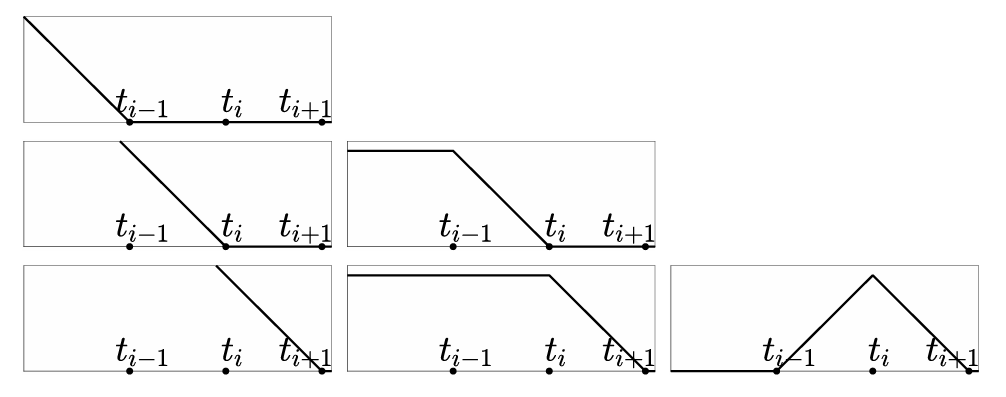
\includegraphics[width=0.6\textwidth]{images/truncated_power_functions.png}
% 仅占位说明:图 3.2 为示意图,展示对截断幂函数做差商的过程及其得到的局部支撑形状(折线图)。
\caption{截断幂函数的差商。}
\label{fig::dd_truncated_power}
\end{figure}

\begin{theorem}
    % thm 3.32
    \label{thm::bspline_as_divdiff_truncated}
(将 B- 样条表示为截断幂函数的差商。)对任意 $n\in\mathbb{N}$, 有
\begin{equation}
    % eq 3.38
\label{eq::Bn_divdiff_truncated}
B^{\,n}_i(x)=(t_{i+n}-t_{i-1})\cdot [t_{i-1},\ldots,t_{i+n}](t-x)^{n}_{+}.
\end{equation}
\end{theorem}

\begin{proof}
当 $n=0$ 时,式 \eqref{eq::Bn_divdiff_truncated} 化为
\[
B^{\,0}_i(x)=(t_i-t_{i-1})\cdot [t_{i-1},t_i](t-x)^{0}_{+}
=(t_i-x)^{0}_{+}-(t_{i-1}-x)^{0}_{+}
=\begin{cases}
0, & x\in(-\infty,t_{i-1}],\\
1, & x\in(t_{i-1},t_i],\\
0, & x\in(t_i,+\infty),
\end{cases}
\]
与式 \eqref{eq::bspline_degree0} 相同,故归纳基成立。现假设归纳假设 \eqref{eq::Bn_divdiff_truncated} 对 $n$ 成立。

由定义 \ref{def::truncated_power},有
\[
(t-x)^{n+1}_{+}=(t-x)\,(t-x)^{n}_{+}.
\]
对 $f=(t-x)$、$g=(t-x)^{n}_{+}$ 应用莱布尼茨公式(定理 \ref{thm::leibniz_divided_difference})(除了$[t_{i-1}](t - x)$ 和 $[t_{i - 1}, t_i](t - x)$ 其余都是 $0$)得
\begin{equation}
    % eq 3.39
\label{eq::leibniz_for_truncated}
\begin{aligned}
&\relax [t_{i-1},\ldots,t_{i+n}](t-x)^{n+1}_{+} \\
=&(t_{i-1}-x)\cdot [t_{i-1},\ldots,t_{i+n}](t-x)^{n}_{+}
+[t_i,\ldots,t_{i+n}](t-x)^{n}_{+}.    
\end{aligned}
\end{equation}

由定义 \ref{def::bspline_recursive} 与归纳假设可得
\[
B^{n+1}_i(x)=\beta(x)+\gamma(x),
\]
其中(用归纳假设)
\[
\begin{aligned}
\beta(x)&=\frac{x-t_{i-1}}{t_{i+n}-t_{i-1}}B^{n}_i(x) \\
&=(x-t_{i-1})\cdot [t_{i-1},\ldots,t_{i+n}](t-x)^{n}_{+} \\
&=[t_i,\ldots,t_{i+n}](t-x)^{n}_{+}-[t_{i-1},\ldots,t_{i+n}](t-x)^{n+1}_{+},    
\end{aligned}
\]
最后一步由式 \eqref{eq::leibniz_for_truncated} (反过来用)得到。类似地,
\[
\gamma(x)=\frac{t_{i+n+1}-x}{t_{i+n+1}-t_i}\,B^{\,n}_{i+1}(x)
=(t_{i+n+1}-x)\cdot [t_i,\ldots,t_{i+n+1}](t-x)^{n}_{+}
\]
\[
=(t_{i+n+1}-t_i)\cdot [t_i,\ldots,t_{i+n+1}](t-x)^{n}_{+}
+(t_i-x)\cdot [t_i,\ldots,t_{i+n+1}](t-x)^{n}_{+}
\]
(加一项减一项)
\[
\begin{aligned}
=[t_{i+1},\ldots,t_{i+n+1}](t-x)^{n}_{+}
-[t_i,\ldots,t_{i+n}](t-x)^{n}_{+} \\
+[t_i,\ldots,t_{i+n+1}](t-x)^{n+1}_{+}
-[t_{i+1},\ldots,t_{i+n+1}](t-x)^{n}_{+},    
\end{aligned}
\]
\[
=[t_i,\ldots,t_{i+n+1}](t-x)^{n+1}_{+}-[t_i,\ldots,t_{i+n}](t-x)^{n}_{+} \\
\]
其中倒数第二步(头两项)由定理 \ref{thm:DD-recursion} 与(后两项)式 \eqref{eq::leibniz_for_truncated} 得到。

由上述结果可得
\[
\begin{aligned}
B^{n+1}_i(x)&=[t_i,\ldots,t_{i+n+1}](t-x)^{n+1}_{+}
-[t_{i-1},\ldots,t_{i+n}](t-x)^{n+1}_{+} \\
&=(t_{i+n+1}-t_{i-1})\cdot [t_{i-1},\ldots,t_{i+n+1}](t-x)^{n+1}_{+},   
\end{aligned}
\]
从而完成归纳证明。
\end{proof}

\begin{remark}
    % remark 3.29
    \label{rem::alt_def_bspline}
有些作者以式 \eqref{eq::Bn_divdiff_truncated} 作为 B- 样条的定义,然后由此推得递推式 \eqref{eq::bspline_recursion}。
\end{remark}

\begin{remark*}
    总结:对 $\mathbb{S}_{n, N}^{n - 1}$ 空间,我们已经构建了一组基:即截断幂函数基(见引理 \ref{lem::tp_basis} 和推论 \ref{cor::tp_expansion});
进一步,我们试图构建一组具有局部支撑性的基:即 B-样条基(见定义 \ref{def::bspline_recursive})。
借助工具莱布尼兹公式(定理 \ref{thm::leibniz_divided_difference}),
我们将 B-样条与截断幂函数联系起来(见定理 \ref{thm::bspline_as_divdiff_truncated})。注意,到这个阶段,
我们还没有证明 B-样条基确实构成 $\mathbb{S}_{n, N}^{n - 1}$ 的一个基。为了完成这一点,我们需要进一步了解 B-样条基的性质,以及更多的形式工具。
\end{remark*}


\subsubsection{积分和导数}
% subsubsec 3.2.3
\label{subsec::bspline_integration_derivation}

\begin{corollary}[B 样条的积分]
% cor 3.33
\label{cor::bspline_integral}
B-样条在其支集上的平均值仅取决于其次数,
\begin{equation}
    % eq 3.40
\label{eq::bspline_average_value}
\frac{1}{t_{i+n} - t_{i-1}} \int_{t_{i-1}}^{t_{i+n}} B_i^n(x) \, dx = \frac{1}{n+1}. 
\end{equation}
\end{corollary}

\begin{proof}
式 (\ref{eq::bspline_average_value}) 的左边(LHS)为
\begin{align*}
&\frac{1}{t_{i+n} - t_{i-1}} \int_{t_{i-1}}^{t_{i+n}} B_i^n(x) \, dx \mbox{(直接使用定理 \ref{thm::bspline_as_divdiff_truncated})}\\
&= \int_{t_{i-1}}^{t_{i+n}} [t_{i-1}, \ldots, t_{i+n}] (t - x)_+^n \, dx\mbox{(积分和差商都是线性泛函)} \\
&= [t_{i-1}, \ldots, t_{i+n}] \int_{t_{i-1}}^{t_{i+n}} (t - x)_+^n \, dx\mbox{(截断幂函数可直接积分,见\eqref{eq::tp_int})} \\
&= [t_{i-1}, \ldots, t_{i+n}] \frac{(t - t_{i-1})^{n+1}}{n+1}\mbox{($(t - t_{i-1})^{n+1}$在$t_{i-1}, \ldots, t_{i+n}$上插值就是自己,最高项系数是 $1$.)} \\
&= \frac{1}{n+1},
\end{align*}
其中第一步由定理 \ref{thm::bspline_as_divdiff_truncated} 得出,第二步由积分与差商运算的交换性得出,
第三步由式 \eqref{eq::tp_int} 得出,最后一步由推论 \ref{cor::newton_remainder} 得出。
\end{proof}

\begin{remark}
    % remark 3.30
事实上,定义 \ref{def::newton_interpolating} 直接推出
\[
[t_{i-1}, \ldots, t_{i+n}] (t - t_{i-1})^{n+1} = 1,
\]
因为插值函数 $(t - t_{i-1})^{n+1}$ 在 $n+2$ 个点 $t_{i-1}, \ldots, t_{i+n}$ 上的插值多项式就是其本身,
且单项式 $t^{n+1}$ 的系数显然为 $1$. 有时这种思维方式既方便又强大;例如,\eqref{eq::leibniz_for_truncated} 可通过这种方式加以证明。(如何?)
\end{remark}

\begin{remark}
    % remark 3.31
当 $n = 1$ 时,推论 \ref{cor::bspline_integral} 简单地说明:三角形的面积仅依赖于其底边和高。
\end{remark}

\begin{theorem}[B-样条的导数]
% thm 3.34
\label{thm::bspline_derivative}
对于 $n \geq 2$, 有 $\forall x \in \mathbb{R}$,
\begin{equation}
    % eq 3.41
\label{eq::bspline_derivative}
\frac{d}{dx} B_i^n(x) = \frac{n B_i^{n-1}(x)}{t_{i+n-1} - t_{i-1}} - \frac{n B_{i+1}^{n-1}(x)}{t_{i+n} - t_i}. 
\end{equation}
当 $n = 1$ 时,式 \eqref{eq::bspline_derivative} 对所有 $x$ 成立,除了三个节点 $t_{i-1}$、$t_i$ 和 $t_{i+1}$ 处,
因为在这些点上 $B_i^1$ 的导数未定义。
\end{theorem}

\begin{proof}
我们首先证明 \eqref{eq::bspline_derivative} 对所有 $x$ 成立,除了在节点 $t_j$ 处。由 \eqref{eq::B1_equals_hat}、\eqref{eq::hat_function} 和 \eqref{eq::bspline_degree0},
我们有:
\[
\forall x \in \mathbb{R} \setminus \{t_{i-1}, t_i, t_{i+1}\}, \quad
\frac{\mathrm{d}}{\mathrm{d}x} B_i^1(x) = \frac{1}{t_i - t_{i-1}} B_i^0(x) - \frac{1}{t_{i+1} - t_i} B_{i+1}^0(x).
\]
因此,归纳基础成立。现在假设 \eqref{eq::bspline_derivative} 对所有 $x \in \mathbb{R} \setminus \{t_{i-1}, \ldots, t_{i+n}\}$ 成立。对 \eqref{eq::bspline_recursion} 求导,
应用归纳假设 \eqref{eq::bspline_derivative},我们得到:
\begin{equation}
    % eq 3.42
\label{eq::bspline_derivative_induction}
\frac{\mathrm{d}}{\mathrm{d}x} B_i^{n+1}(x) = \frac{B_i^n(x)}{t_{i+n} - t_{i-1}} - \frac{B_{i+1}^n(x)}{t_{i+n+1} - t_i} + n C(x), 
\end{equation}
其中 $C(x)$ 为(求导的乘法法则):
\begin{align*}
&\frac{x - t_{i-1}}{t_{i+n} - t_{i-1}} \left[ \frac{B_i^{n-1}(x)}{t_{i+n-1} - t_{i-1}} - \frac{B_{i+1}^{n-1}(x)}{t_{i+n} - t_i} \right] \\
+ &\frac{t_{i+n+1} - x}{t_{i+n+1} - t_i} \left[ \frac{B_{i+1}^{n-1}(x)}{t_{i+n} - t_i} - \frac{B_{i+2}^{n-1}(x)}{t_{i+n+1} - t_{i+1}} \right] \\
= &\frac{1}{t_{i+n} - t_{i-1}} \left[ \frac{(x - t_{i-1}) B_i^{n-1}(x)}{t_{i+n-1} - t_{i-1}} + \frac{(t_{i+n} - x) B_{i+1}^{n-1}(x)}{t_{i+n} - t_i} \right] \\
- &\frac{1}{t_{i+n+1} - t_i} \left[ \frac{(x - t_i) B_{i+1}^{n-1}(x)}{t_{i+n} - t_i} + \frac{(t_{i+n+1} - x) B_{i+2}^{n-1}(x)}{t_{i+n+1} - t_{i+1}} \right] \\
= &\frac{B_i^n(x)}{t_{i+n} - t_{i-1}} - \frac{B_{i+1}^n(x)}{t_{i+n+1} - t_i},
\end{align*}
其中最后一步由 \eqref{eq::bspline_recursion} 得出。于是 \eqref{eq::bspline_derivative_induction} 可写为:
\[
\frac{\mathrm{d}}{\mathrm{d}x} B_i^{n+1}(x) = \frac{(n+1) B_i^n(x)}{t_{i+n} - t_{i-1}} - \frac{(n+1) B_{i+1}^n(x)}{t_{i+n+1} - t_i},
\]
这完成了 \eqref{eq::bspline_derivative} 的归纳证明,除了在节点处。由于 $B_i^1 = \hat{B}_i$ 是连续的,
结合 \eqref{eq::bspline_recursion} 进行简单的归纳可得:对所有 $n \geq 1$, $B_i^n$ 都是连续的。因此,\eqref{eq::bspline_derivative} 的右边对所有 $n \geq 2$ 都是连续的。
所以,当 $n \geq 2$ 时,$\frac{\mathrm{d}}{\mathrm{d}x} B_i^n(x)$ 对所有 $x \in \mathbb{R}$ 都存在。这就完成了证明。

\end{proof}

\begin{remark*}
目标是证明
\[
C(x)=\frac{B^{n}_i(x)}{t_{i+n}-t_{i-1}}-\frac{B^{n}_{i+1}(x)}{t_{i+n+1}-t_i}.
\]

从原始表达式出发:
\begin{align*}
C(x)
&=\frac{x-t_{i-1}}{t_{i+n}-t_{i-1}}
\Biggl[
\frac{B^{n-1}_i(x)}{t_{i+n-1}-t_{i-1}}-\frac{B^{n-1}_{i+1}(x)}{t_{i+n}-t_i}
\Biggr]
+\frac{t_{i+n+1}-x}{t_{i+n+1}-t_i}
\Biggl[
\frac{B^{n-1}_{i+1}(x)}{t_{i+n}-t_i}-\frac{B^{n-1}_{i+2}(x)}{t_{i+n+1}-t_{i+1}}
\Biggr].
\end{align*}

第 1 步(重排并按公共外因子分组):
\begin{align*}
C(x)
&=\frac{1}{t_{i+n}-t_{i-1}}
\Biggl[
\frac{(x-t_{i-1})B^{n-1}_i(x)}{t_{i+n-1}-t_{i-1}}
+\frac{(t_{i+n}-x)B^{n-1}_{i+1}(x)}{t_{i+n}-t_i}
\Biggr]\\
&\quad-\frac{1}{t_{i+n+1}-t_i}
\Biggl[
\frac{(x-t_i)B^{n-1}_{i+1}(x)}{t_{i+n}-t_i}
+\frac{(t_{i+n+1}-x)B^{n-1}_{i+2}(x)}{t_{i+n+1}-t_{i+1}}
\Biggr].
\end{align*}
说明:使用恒等式
\[
(x-t_{i-1})+(t_{i+n}-x)=t_{i+n}-t_{i-1},\qquad
(x-t_i)+(t_{i+n+1}-x)=t_{i+n+1}-t_i,
\]
将与 $B^{n-1}_{i+1}$ 相关的两项分别并入对应方括号中。

第 2 步(识别 de Boor 递推结构):
\begin{align*}
\Biggl[
\frac{(x-t_{i-1})B^{n-1}_i}{t_{i+n-1}-t_{i-1}}
+\frac{(t_{i+n}-x)B^{n-1}_{i+1}}{t_{i+n}-t_i}
\Biggr]&=B^{n}_i(x),\\
\Biggl[
\frac{(x-t_i)B^{n-1}_{i+1}}{t_{i+n}-t_i}
+\frac{(t_{i+n+1}-x)B^{n-1}_{i+2}}{t_{i+n+1}-t_{i+1}}
\Biggr]&=B^{n}_{i+1}(x),
\end{align*}
这正是 B 样条的递推公式(de Boor 公式)的两种索引实例。

由此得到最终结果:
\[
C(x)=\frac{B^{n}_i(x)}{t_{i+n}-t_{i-1}}-\frac{B^{n}_{i+1}(x)}{t_{i+n+1}-t_i}.
\]    

下面把“第 1 步(重排并按公共外因子分组)”写成逐项等价变形。

从原式
\[
\begin{aligned}
C(x)
&=\frac{x-t_{i-1}}{t_{i+n}-t_{i-1}}
\Biggl(
\frac{B^{n-1}_i(x)}{t_{i+n-1}-t_{i-1}}
-\frac{B^{n-1}_{i+1}(x)}{t_{i+n}-t_i}
\Biggr)
+\frac{t_{i+n+1}-x}{t_{i+n+1}-t_i}
\Biggl(
\frac{B^{n-1}_{i+1}(x)}{t_{i+n}-t_i}
-\frac{B^{n-1}_{i+2}(x)}{t_{i+n+1}-t_{i+1}}
\Biggr)
\end{aligned}
\]
出发,先把外层系数分配进每个括号(逐项乘开):
\[
\begin{aligned}
C(x)
&=\frac{x-t_{i-1}}{t_{i+n}-t_{i-1}}\cdot
\frac{B^{n-1}_i(x)}{t_{i+n-1}-t_{i-1}}
-\frac{x-t_{i-1}}{t_{i+n}-t_{i-1}}\cdot
\frac{B^{n-1}_{i+1}(x)}{t_{i+n}-t_i} \\
&\quad+\frac{t_{i+n+1}-x}{t_{i+n+1}-t_i}\cdot
\frac{B^{n-1}_{i+1}(x)}{t_{i+n}-t_i}
-\frac{t_{i+n+1}-x}{t_{i+n+1}-t_i}\cdot
\frac{B^{n-1}_{i+2}(x)}{t_{i+n+1}-t_{i+1}}.
\end{aligned}
\]

现在把与 $B^{n-1}_i$、$B^{n-1}_{i+2}$ 的两项分别保持不动,把与
$B^{n-1}_{i+1}$ 的两项合并为“两个带不同公共因子”的组。具体做法是分别把
$\dfrac{1}{t_{i+n}-t_{i-1}}$ 与 $\dfrac{1}{t_{i+n+1}-t_i}$ 提到每组外面:

1) 关于 $B^{n-1}_i$ 与 $B^{n-1}_{i+1}$ 的第一组(提取 $1/(t_{i+n}-t_{i-1})$):
\[
\frac{x-t_{i-1}}{t_{i+n}-t_{i-1}}\cdot
\frac{B^{n-1}_i(x)}{t_{i+n-1}-t_{i-1}}
-\frac{x-t_{i-1}}{t_{i+n}-t_{i-1}}\cdot
\frac{B^{n-1}_{i+1}(x)}{t_{i+n}-t_i}.
\]
将第二项中的系数
$-\dfrac{x-t_{i-1}}{t_{i+n}-t_{i-1}}$
改写为
\[
-\frac{x-t_{i-1}}{t_{i+n}-t_{i-1}}
=\frac{t_{i+n}-x}{t_{i+n}-t_{i-1}}-1
\qquad (\text{因为 }(t_{i+n}-x)-(x-t_{i-1})=t_{i+n}-t_{i-1}),
\]
于是这一组可重写为
\[
\frac{1}{t_{i+n}-t_{i-1}}
\Biggl[
\frac{(x-t_{i-1})B^{n-1}_i(x)}{t_{i+n-1}-t_{i-1}}
+\frac{(t_{i+n}-x)B^{n-1}_{i+1}(x)}{t_{i+n}-t_i}
\Biggr]
-\frac{B^{n-1}_{i+1}(x)}{t_{i+n}-t_i}.
\]
这里我们有意地把“$-1\cdot\dfrac{B^{n-1}_{i+1}}{t_{i+n}-t_i}$”暂时留在组外,待会儿与下一组合并。

2) 关于 $B^{n-1}_{i+1}$ 与 $B^{n-1}_{i+2}$ 的第二组(提取 $1/(t_{i+n+1}-t_i)$):
\[
\frac{t_{i+n+1}-x}{t_{i+n+1}-t_i}\cdot
\frac{B^{n-1}_{i+1}(x)}{t_{i+n}-t_i}
-\frac{t_{i+n+1}-x}{t_{i+n+1}-t_i}\cdot
\frac{B^{n-1}_{i+2}(x)}{t_{i+n+1}-t_{i+1}}.
\]
将第一项中的系数
$\dfrac{t_{i+n+1}-x}{t_{i+n+1}-t_i}$
改写为
\[
\frac{t_{i+n+1}-x}{t_{i+n+1}-t_i}
=1-\frac{x-t_i}{t_{i+n+1}-t_i}
\qquad (\text{因为 }(t_{i+n+1}-x)+(x-t_i)=t_{i+n+1}-t_i),
\]
于是这一组可重写为
\[
\frac{B^{n-1}_{i+1}(x)}{t_{i+n}-t_i}
-\frac{1}{t_{i+n+1}-t_i}
\Biggl[
\frac{(x-t_i)B^{n-1}_{i+1}(x)}{t_{i+n}-t_i}
+\frac{(t_{i+n+1}-x)B^{n-1}_{i+2}(x)}{t_{i+n+1}-t_{i+1}}
\Biggr].
\]

将两组结果与上一步遗留的
$-\dfrac{B^{n-1}_{i+1}(x)}{t_{i+n}-t_i}$ 相加,恰好抵消:
\[
-\frac{B^{n-1}_{i+1}(x)}{t_{i+n}-t_i}
+\frac{B^{n-1}_{i+1}(x)}{t_{i+n}-t_i}=0.
\]
因此 $C(x)$ 化为
\[
\boxed{
\begin{aligned}
C(x)
&=\frac{1}{t_{i+n}-t_{i-1}}
\Biggl[
\frac{(x-t_{i-1})B^{n-1}_i(x)}{t_{i+n-1}-t_{i-1}}
+\frac{(t_{i+n}-x)B^{n-1}_{i+1}(x)}{t_{i+n}-t_i}
\Biggr]\\
&\quad-\frac{1}{t_{i+n+1}-t_i}
\Biggl[
\frac{(x-t_i)B^{n-1}_{i+1}(x)}{t_{i+n}-t_i}
+\frac{(t_{i+n+1}-x)B^{n-1}_{i+2}(x)}{t_{i+n+1}-t_{i+1}}
\Biggr],
\end{aligned}}
\]
这就是“第 1 步”的目标形式。接下来第 2 步只需识别每个方括号都是
B 样条的 de Boor 递推组合,从而得到
$C(x)=\dfrac{B^{n}_i(x)}{t_{i+n}-t_{i-1}}
-\dfrac{B^{n}_{i+1}(x)}{t_{i+n+1}-t_i}$。
\end{remark*}

\begin{remark}
另一种方式,定理 \ref{thm::bspline_derivative} 可以从定理 \ref{thm::bspline_as_divdiff_truncated} 推导如下:
\begin{align*}
\frac{\mathrm{d}}{\mathrm{d}x} B_i^n(x) &= (t_{i+n} - t_{i-1}) \cdot [t_{i-1}, \ldots, t_{i+n}] \frac{\mathrm{d}}{\mathrm{d}x} (t - x)_+^n \\
&= ([t_i, \ldots, t_{i+n}] - [t_{i-1}, \ldots, t_{i+n-1}]) (-n (t - x)_+^{n-1}) \\
&= n [t_{i-1}, \ldots, t_{i+n-1}] (t - x)_+^{n-1} - n [t_i, \ldots, t_{i+n}] (t - x)_+^{n-1} \\
&= \frac{n B_i^{n-1}(x)}{t_{i+n-1} - t_{i-1}} - \frac{n B_{i+1}^{n-1}(x)}{t_{i+n} - t_i},
\end{align*}
其中第二行由定理 \ref{thm:DD-recursion} 得出。

推论 \ref{cor::bspline_integral} 可以部分地从定理 \ref{thm::bspline_derivative} 推出。

\[
\begin{aligned}
& \int_{t_{i-1}}^{t_{i+n}} \frac{\mathrm{d}}{\mathrm{d}x} B_i^n(x) \, dx = 0 \\
\Rightarrow & \frac{\displaystyle \int_{t_{i-1}}^{t_{i+n}} B_i^{n-1}(x) \, dx}{t_{i+n-1} - t_{i-1}} = \frac{\displaystyle \int_{t_{i-1}}^{t_{i+n}} B_{i+1}^{n-1}(x) \, dx}{t_{i+n} - t_i}. \\
\Rightarrow & \frac{\displaystyle \int_{t_{i-1}}^{t_{i+n-1}} B_i^{n-1}(x) \, dx}{t_{i+n-1} - t_{i-1}} = \frac{\displaystyle \int_{t_i}^{t_{i+n}} B_{i+1}^{n-1}(x) \, dx}{t_{i+n} - t_i}. \\
\Rightarrow & \frac{\displaystyle \int_{t_{i-1}}^{t_{i+n}} B_i^n(x) \, dx}{t_{i+n} - t_{i-1}} = \frac{\displaystyle \int_{t_i}^{t_{i+n+1}} B_{i+1}^n(x) \, dx}{t_{i+n+1} - t_i},
\end{aligned}
\]
其中第一行由微积分基本定理和引理 \ref{lem::support_bspline} 得出,第二行由定理 \ref{thm::bspline_derivative} 得出,
第三行由引理 \ref{lem::support_bspline} 得出,最后一行是将 $n$ 替换为 $n+1$.  (只得到都相等。)  
\end{remark}

\begin{corollary}[B 样条的光滑性]
    % cor 3.35
    \label{cor::bspline_higher_derivative}
    $B_i^n \in \mathbb{S}_n^{n-1}$.
\end{corollary}

\begin{proof}
当 $n=1$ 时,归纳基础 $B_i^1(x) \in \mathbb{S}_1^0$ 成立,这是由 \eqref{eq::B1_equals_hat} 得出的。其余部分的证明由 \eqref{eq::bspline_recursion} 
和定理 \ref{thm::bspline_derivative} 通过简单的归纳法即可得出。
\end{proof}

\subsubsection{Marsden 恒等式}
% subsec 3.2.4
\label{subsubsec::marsden_identity}

\begin{theorem}[Marsden 恒等式]
    % thm 3.36
    \label{thm::marsden_identity}
对任意 $n\in\mathbb{N}$, 有
\begin{equation}
    % eq 3.43
\label{eq::marsden_identity}
(t-x)^n=\sum_{i=-\infty}^{+\infty}(t-t_i)\cdots (t-t_{i+n-1})\,B^{\,n}_i(x),
\end{equation}
其中当 $n=0$ 时,乘积 $(t-t_i)\cdots (t-t_{i+n-1})$ 按约定取为 $1$.
\end{theorem}

(右边加起来是个函数。)

\begin{proof}
当 $n=0$ 时,式 \eqref{eq::marsden_identity} 由定义 \ref{def::bspline_recursive} 推出。现在假设式 \eqref{eq::marsden_identity} 成立。
线性函数 $f(t)=t-x$ 的线性插值就是其自身,即(插值点是 $t_{i-1}, t_{i+n}$)
\begin{equation}
    % eq 3.44
\label{eq::linear_interp_t_minus_x}
t-x=\frac{t-t_{i+n}}{t_{i-1}-t_{i+n}}\,(t_{i-1}-x)+\frac{t-t_{i-1}}{t_{i+n}-t_{i-1}}\,(t_{i+n}-x).
\end{equation}
于是归纳步有
\[
\begin{aligned}
(t-x)^{n+1}
&=(t-x)\sum_{i=-\infty}^{+\infty}(t-t_i)\cdots (t-t_{i+n-1})\,B^{\,n}_i(x) \\
&=\sum_{i=-\infty}^{+\infty}(t-t_i)\cdots (t-t_{i+n}) 
\frac{t_{i-1}-x}{t_{i-1}-t_{i+n}}\,B^{\,n}_i(x) \\
&+\sum_{i=-\infty}^{+\infty}(t-t_{i-1})\cdots (t-t_{i+n-1})
\frac{t_{i+n}-x}{t_{i+n}-t_{i-1}}\,B^{\,n}_i(x) \mbox{(注意第二项乘最前面)}\\
&=\sum_{i=-\infty}^{+\infty}(t-t_i)\cdots (t-t_{i+n})
\frac{x-t_{i-1}}{t_{i+n}-t_{i-1}}\,B^{\,n}_i(x) \mbox{(分子分母同换)}\\
&+\sum_{i=-\infty}^{+\infty}(t-t_i)\cdots (t-t_{i+n})
\frac{t_{i+n+1}-x}{t_{i+n+1}-t_i}\,B^{\,n}_{i+1}(x) \mbox{(指标加 $1$)}\\
&=\sum_{i=-\infty}^{+\infty}(t-t_i)\cdots (t-t_{i+n})\,B^{\,n+1}_i(x),
\end{aligned}
\]
其中第一步来自归纳假设,第二步来自式 \eqref{eq::linear_interp_t_minus_x},第三步由第二个求和式中将指标 $i$ 替换为 $i+1$ 得到,最后一步来自式 \eqref{eq::bspline_recursion}。
\end{proof}

\begin{corollary}
    % cor 3.37
    \label{cor::truncated_as_linear_comb_bspline}
(将截断幂函数表示为 B- 样条的线性组合)。对任意 $j\in\mathbb{Z}$ 和 $n\in\mathbb{N}$, 有
\begin{equation}
    % eq 3.45
\label{eq::truncated_linear_combo}
(t_j-x)^{n}_{+}=\sum_{i=-\infty}^{j-n}(t_j-t_i)\cdots (t_j-t_{i+n-1})\,B^{\,n}_i(x).
\end{equation}
\end{corollary}

\begin{proof}
我们需要证明右端在 $x\le t_j$ 时等于 $(t_j-x)^n$, 否则为 $0$. 在式 \eqref{eq::marsden_identity} 中取 $t=t_j$, 得到
\[
(t_j-x)^n=\sum_{i=-\infty}^{+\infty}(t_j-t_i)\cdots (t_j-t_{i+n-1})\,B^{\,n}_i(x).
\]
对每个 $i=j-n+1,\ldots,j$, 上述求和中的相应项与 $x$ 无关恒为 $0$; 而对每个 $i\ge j+1$, 引理 \ref{lem::support_bspline} 蕴含(支撑之外都是零。)当 $x\le t_j$ 时 $B^{\,n}_i(x)=0$. 因此
\[
x\le t_j\ \Longrightarrow\ \sum_{i=-\infty}^{j-n}(t_j-t_i)\cdots (t_j-t_{i+n-1})\,B^{\,n}_i(x)=(t_j-x)^n.
\]
若 $x>t_j$, 则由引理 \ref{lem::support_bspline} 得 $B^{\,n}_i(x)=0$ 对所有 $i\le j-n$ 均成立。证毕。
\end{proof}

\subsubsection{对称多项式}
% subsec 3.2.5
\label{subsubsec::symmetric_polynomials}

\begin{definition}
    % def 3.38
    \label{def::elementary_symmetric_poly}
(基本对称多项式)在 $n$ 个变量中的次数为 $k$ 的基本对称多项式,是从这 $n$ 个变量中选取 $k$ 个互不相同的变量所得到的所有乘积之和,即
\begin{equation}
    % eq 3.46
\label{eq::elem_sym_def}
\sigma_k(x_1,\ldots,x_n)=
\sum_{1\le i_1<\cdots<i_k\le n} x_{i_1}x_{i_2}\cdots x_{i_k}.
\end{equation}
特别地,$\sigma_0(x_1,\ldots,x_n)=1$,并且
\[
\forall\,k>n,\qquad \sigma_k(x_1,\ldots,x_n)=0.
\]
若去掉“互不相同”的条件,则得到在 $n$ 个变量中的次数为 $k$ 的完全对称多项式:
\begin{equation}
    % eq 3.47
\label{eq::complete_sym_def}
\tau_k(x_1,\ldots,x_n)=
\sum_{1\le i_1\le\cdots\le i_k\le n} x_{i_1}x_{i_2}\cdots x_{i_k}.
\end{equation}
\end{definition}

\begin{example}
    % ex 3.39
    \label{ex::elem_sym_239}
$\sigma_2(x_1,x_2,x_3)=x_1x_2+x_1x_3+x_2x_3$. 作比较,$\tau_2(x_1,x_2,x_3)=\sigma_2(x_1,x_2,x_3)+x_1^2+x_2^2+x_3^2$.
\end{example}

\begin{lemma}
    % lem 3.40
    \label{lem::elem_sym_recursion}
当 $k\le n$ 时,基本对称多项式满足如下递推关系:
\begin{equation}
    % eq 3.48
\label{eq::elem_sym_rec}
\sigma_{k+1}(x_1,\ldots,x_n,x_{n+1})
=\sigma_{k+1}(x_1,\ldots,x_n)+x_{n+1}\,\sigma_k(x_1,\ldots,x_n).
\end{equation}
\end{lemma}

\begin{proof}
$\sigma_{k+1}(x_1,\ldots,x_n,x_{n+1})$ 中的各项可分为两类:
(a) 含有因子 $x_{n+1}$ 的项;
(b) 不含该因子的项。由式 \eqref{eq::elem_sym_def} 的对称性可知,(a) 类恰为 $x_{n+1}\sigma_k(x_1,\ldots,x_n)$,(b) 类恰为 $\sigma_{k+1}(x_1,\ldots,x_n)$. 故得结论。
\end{proof}

\begin{example}
    % ex 3.41
    \label{ex::elem_sym_241}
$\sigma_2(x_1,x_2,x_3)=x_1x_2+x_3(x_1+x_2)$.
\end{example}

\begin{definition}
    % def 3.42
    \label{def::gen_func_elementary}
基本对称多项式的生成函数为
\begin{equation}
    % eq 3.49
\label{eq::gen_func_sigma}
g_{\sigma,n}(z)=\prod_{i=1}^{n}(1+x_i z)=(1+x_1 z)\cdots(1+x_n z).
\end{equation}
对于完全对称多项式,其生成函数为
\begin{equation}
    % eq 3.50
\label{eq::gen_func_tau}
g_{\tau,n}(z)=\prod_{i=1}^{n}\frac{1}{1-x_i z}
=\frac{1}{1-x_1 z}\cdots\frac{1}{1-x_n z}.
\end{equation}
\end{definition}

\begin{lemma}
    % lem 3.43
    \label{lem::gen_elem_complete}
(生成基本对称与完全对称多项式)。基本对称与完全对称多项式与其生成函数之间满足
\begin{align}
    % eq 3.51
    \label{eq::gen_func_sigma_expansion}
g_{\sigma,n}(z)&=\sum_{k=0}^{n}\sigma_k(x_1,\ldots,x_n)\,z^k,
\\
    % eq 3.52
    \label{eq::gen_func_tau_expansion}
g_{\tau,n}(z)&=\sum_{k=0}^{+\infty}\tau_k(x_1,\ldots,x_n)\,z^k.
\end{align}
\end{lemma}

\begin{proof}
结合引理 \ref{lem::elem_sym_recursion},式 \eqref{eq::gen_func_sigma_expansion} 可用简单的归纳法证明。对于式 \eqref{eq::gen_func_tau_expansion},
由式 \eqref{eq::gen_func_tau} 以及恒等式
\begin{equation}
    % eq 3.53
\label{eq::geom_series_identity}
\frac{1}{1-x}=\sum_{k=0}^{+\infty}x^k
\end{equation}
得到
\[
g_{\tau,n}(z)=\prod_{i=1}^{n}\sum_{k=0}^{+\infty}x_i^{\,k}z^{k}
=(1+x_1 z+x_1^{2}z^{2}+\cdots)(1+x_2 z+x_2^{2}z^{2}+\cdots)\cdots
(1+x_n z+x_n^{2}z^{2}+\cdots).
\]
$z^k$ 的单项式系数等于从 $x_1,x_2,\ldots,x_n$ 中取 $k$ 个变量的所有乘积之和。由定义 \ref{def::elementary_symmetric_poly} 即得结论。
\end{proof}

\begin{remark}
    % rem 3.33
    \label{rem::geom_series_algebraic}
恒等式 \eqref{eq::geom_series_identity} 成立,因为
\[
1\equiv (1-x)\sum_{k=0}^{+\infty}x^k
=\sum_{k=0}^{+\infty}x^k-\sum_{k=1}^{+\infty}x^k.
\]
这是一个代数层面的论证,与几何级数收敛所需的 $|x|<1$ 条件无关,原因是:
(i) 这里的 $x$ 不是数而是符号;
(ii) \eqref{eq::geom_series_identity} 仅用于识别两个等价多项式的系数,这与几何级数的收敛性无关。
\end{remark}

\begin{example}
    % ex 3.44
    \label{ex::gen_example_344}
\[
(1+x_1 z)(1+x_2 z)(1+x_3 z)
=1+(x_1+x_2+x_3)z+(x_1x_2+x_1x_3+x_2x_3)z^2+x_1x_2x_3 z^3.
\]
\end{example}

\begin{lemma}
    % lem 3.45
    \label{lem::tau_recursion}
(完全对称多项式的递推关系)。完全对称多项式满足如下递推:
\begin{equation}
    % eq 3.54
\label{eq::tau_recursion}
\tau_{k+1}(x_1,\ldots,x_n,x_{n+1})
=\tau_{k+1}(x_1,\ldots,x_n)+x_{n+1}\,\tau_k(x_1,\ldots,x_n,x_{n+1}).
\end{equation}
\end{lemma}

\begin{proof}
由式 \eqref{eq::gen_func_tau} 可得
\begin{equation}
    % eq 3.55
\label{eq::gen_tau_shift}
g_{\tau,n+1}=g_{\tau,n}+x_{n+1}z\,g_{\tau,n+1}.
\end{equation}
令等式两边 $z^{k+1}$ 的系数相等,即得结论。
\end{proof}

\begin{remark}
    % rem 3.34
    \label{rem::deduce_sigma_from_tau}
通过删除每一项中含有重复 $x_i$ 因子的项,可以由引理 \ref{lem::tau_recursion} 推出引理 \ref{lem::elem_sym_recursion}。
此外,引理 \ref{lem::elem_sym_recursion} 中的条件 $k\le n$ 在引理 \ref{lem::tau_recursion} 中并未出现。
\end{remark}

\begin{theorem}
    % thm 3.46
    \label{thm::tau_as_divdiff}
(完全对称多项式即单项式的差商)。在 $n+1$ 个变量中的次数为 $m-n$ 的完全对称多项式是单项式 $x^{m}$ 的第 $n$ 阶差商,即
\begin{equation}
    % eq 3.56
\label{eq::tau_divdiff}
\forall m\in\mathbb{N}^+,\ \forall i\in\mathbb{N},\ \forall n=0,1,\ldots,m,\qquad
\tau_{m-n}(x_i,\ldots,x_{i+n})=[x_i,\ldots,x_{i+n}]\,x^{m}.
\end{equation}
\end{theorem}

\begin{proof}
由引理 \ref{lem::tau_recursion} 可得
\begin{equation}
    % eq 3.57
\label{eq::tau_recursion_step}
\begin{array}{rl}
& (x_{n+1}-x_1)\,\tau_k(x_1,\ldots,x_n,x_{n+1}) \\
&=\tau_{k+1}(x_1,\ldots,x_n,x_{n+1})-\tau_{k+1}(x_1,\ldots,x_n)\\
&\quad -x_1\,\tau_k(x_1,\ldots,x_n,x_{n+1})\\
&=\tau_{k+1}(x_2,\ldots,x_n,x_{n+1})+x_1\,\tau_k(x_1,\ldots,x_n,x_{n+1})\\
&\quad -\tau_{k+1}(x_1,\ldots,x_n)-x_1\,\tau_k(x_1,\ldots,x_n)\\
&=\tau_{k+1}(x_2,\ldots,x_n,x_{n+1})-\tau_{k+1}(x_1,\ldots,x_n).
\end{array}
\end{equation}
余下部分对 $n$ 作归纳。当 $n=0$ 时,式 \eqref{eq::tau_divdiff} 化为
\[
\tau_m(x_i)=[x_i]\,x^{m},
\]
这显然成立。现在设 \eqref{eq::tau_divdiff} 对某个满足 $n<m$ 的非负整数 $n$ 成立。由式 \eqref{eq::tau_recursion_step} 与归纳假设得到
\[
\begin{aligned}
\tau_{m-n-1}(x_i,\ldots,x_{i+n+1})
&=\frac{\tau_{m-n}(x_{i+1},\ldots,x_{i+n+1})-\tau_{m-n}(x_i,\ldots,x_{i+n})}{x_{i+n+1}-x_i}\\
&=\frac{[x_{i+1},\ldots,x_{i+n+1}]\,x^{m}-[x_i,\ldots,x_{i+n}]\,x^{m}}{x_{i+n+1}-x_i}\\
&=[x_i,\ldots,x_{i+n+1}]\,x^{m},
\end{aligned}
\]
从而完成证明。
\end{proof}

\subsubsection{B 样条确实构成一组基}
\label{subsubsec::bspline_basis}
% subsec 3.2.6

\begin{theorem}
    % thm 3.47
    \label{thm::bspline_basis}
给定任意 $k\in\mathbb{N}$,对任意固定的 $n\ge k$,单项式 $x^{k}$ 都可以表示为 B 样条的线性组合,其形式为
\begin{equation}
    % eq 3.58
\label{eq::monomial_bspline_combo}
\binom{n}{k}x^{k}=\sum_{i=-\infty}^{+\infty}\sigma_k(t_i,\ldots,t_{i+n-1})\,B^{\,n}_i(x),
\end{equation}
其中 $\sigma_k(t_i,\ldots,t_{i+n-1})$ 是关于 $n$ 个变量 $t_i,\ldots,t_{i+n-1}$ 的次数为 $k$ 的基本对称多项式。
\end{theorem}

\begin{proof}
由引理 \ref{lem::gen_elem_complete} 可得
\[
(1+t_i x)\cdots(1+t_{i+n-1}x)=\sum_{k=0}^{n}\sigma_k(t_i,\ldots,t_{i+n-1})\,x^{k}.
\]
将 $x$ 替换为 $-1/t$,并两边同乘 $t^{n}$,得到
\[
(t-t_i)\cdots(t-t_{i+n-1})=\sum_{k=0}^{n}\sigma_k(t_i,\ldots,t_{i+n-1})(-1)^{k}t^{\,n-k}.
\]
把上式代入 \eqref{eq::marsden_identity} 即得
\[
\begin{aligned}
(t-x)^{n}
&=\sum_{i=-\infty}^{+\infty}\sum_{k=0}^{n}\sigma_k(t_i,\ldots,t_{i+n-1})(-1)^{k}t^{\,n-k}B^{\,n}_i(x)\\ 
&=\sum_{k=0}^{n}\Bigl\{t^{\,n-k}(-1)^{k}\sum_{i=-\infty}^{+\infty}\sigma_k(t_i,\ldots,t_{i+n-1})B^{\,n}_i(x)\Bigr\}.
\end{aligned}
\]
另一方面,二项式定理给出
\[
(t-x)^{n}=\sum_{k=0}^{n}\binom{n}{k}t^{\,n-k}(-x)^{k}
=\sum_{k=0}^{n}t^{\,n-k}(-1)^{k}\binom{n}{k}x^{k}.
\]
比较最后两式中 $t^{\,n-k}(-1)^{k}$ 的系数,即得所需结论。
\end{proof}

\begin{remark}
    % rem 3.35
    \label{rem::double_sum_order}
细心的读者也许会质疑在定理 \ref{thm::bspline_basis} 的证明中交换双重求和次序的正当性,
因为在基础分析中我们学到,两重无穷和改变求和次序可能会得出不同的结果。
考虑如下一个无限二维数组 $\{a_{ij}: i,j\in\mathbb{Z}^{+}\}$ 的例子:
\[
a_{ij}=
\begin{cases}
-1, & i=j,\\
2^{\,j-i}, & i>j,\\
0, & i<j,
\end{cases}
\qquad\text{即}\qquad
\begin{array}{cccccc}
-1 & 0 & 0 & 0 & \cdots\\
\frac12 & -1 & 0 & 0 & \cdots\\
\frac14 & \frac12 & -1 & 0 & \cdots\\
\frac18 & \frac14 & \frac12 & -1 & \cdots\\
\vdots & \vdots & \vdots & \vdots & \ddots
\end{array}
\]
容易验证
\[
\sum_{i=1}^{+\infty}\sum_{j=1}^{+\infty}a_{ij}=-2,\qquad
\sum_{j=1}^{+\infty}\sum_{i=1}^{+\infty}a_{ij}=-2,\qquad
\sum_{j=1}^{+\infty}\sum_{i=1}^{+\infty}a_{ij}=0.
\]
然而,在定理 \ref{thm::bspline_basis} 的证明中,按 $k$ 索引的求和只有有限项,
因此上述“反例”并不适用。事实上,对于任意固定的 $x$,按 $i$ 索引的求和中,非零项的个数也是有限的。
因此,对任意给定的 $x$ 与 $n$,表达式 $(t-x)^{n}$ 的双重求和只含有限项。
将 $i$ 的求和范围写成从 $-\infty$ 到 $+\infty$ 仅是一种记号便利,使得对所有 $x\in\mathbb{R}$ 的 $(t-x)^{n}$ 表达式能够采用同一形式。
\end{remark}

\begin{corollary}
    % cor 3.48
    \label{cor::partition_of_unity}
(单位分解)。对任意 $n\in\mathbb{N}$,
\begin{equation}
    % eq 3.59
    \label{eq::partition_of_unity}
\sum_{i=-\infty}^{+\infty} B^{\,n}_i=1.
\end{equation}
\end{corollary}

\begin{proof}
在定理 \ref{thm::bspline_basis} 中取 $k=0$ 即得式 \eqref{eq::partition_of_unity}。
\end{proof}

\begin{remark}
    % rem 3.36
    \label{rem::poU_special_case}
推论 \ref{cor::partition_of_unity} 是定理 D.151 的一个特例。
\end{remark}

\begin{theorem}
    % thm 3.49
    \label{thm::basis_Sn-1}
下列 B 样条组成空间 $S^{\,n-1}_n(t_1,t_2,\ldots,t_N)$ 的一组基:
\begin{equation}
    % eq 3.60
\label{eq::basis_list}
B^{\,n}_{2-n}(x),\ B^{\,n}_{3-n}(x),\ \ldots,\ B^{\,n}_{N}(x).
\end{equation}
\end{theorem}

\begin{proof}
容易验证,对任意 $t_i\in\mathbb{R}$,
\begin{equation}
    % eq 3.61
\label{eq::trunc_identity}
(x-t_i)^{n}_{+}=(x-t_i)^{n}-(-1)^{n}(t_i-x)^{n}_{+}.
\end{equation}
由定理 \ref{thm::marsden_identity} 与推论 \ref{cor::truncated_as_linear_comb_bspline} 可知,
每个截断幂函数 $(x-t_i)^{n}_{+}$ 都可表示为 B 样条的线性组合。由引理 \ref{lem::tp_basis},$S^{\,n-1}_n(t_1,t_2,\ldots,t_N)$ 中的每个元素都可以表示为
\[
1,\ x,\ x^{2},\ldots,x^{n},\ (x-t_2)^{n}_{+},\ (x-t_3)^{n}_{+},\ldots,(x-t_{N-1})^{n}_{+}
\]
的线性组合。定理 \ref{thm::bspline_basis} 说明,每个单项式 $x^{j}$ 亦可表示为 B 样条的线性组合。
由于定义域限制在 $[t_1,t_N]$ 上,依据引理 \ref{lem::support_bspline},
我们知道线性组合中只会出现列表 \eqref{eq::basis_list} 中的那些 B 样条。
因此,这些 B 样条在 $S^{\,n-1}_n(t_1,t_2,\ldots,t_N)$ 中张成。结合引理 B.41、定理 \ref{thm::dim_Sn},
以及列表 \eqref{eq::basis_list} 的长度也为 $n+N-1$ 的事实,证明完毕。 
\end{proof}

\begin{remark}
    % rem 3.37
    \label{rem::alt_proof_basis}
或者,定理 \ref{thm::basis_Sn-1} 也可以用不涉及 \ref{subsubsec::marsden_identity} 与 \ref{subsubsec::symmetric_polynomials} 节内容的方法来证明。

首先,很容易证明
\[
\operatorname{span}\{1,x,\ldots,x^{n}\}
=\operatorname{span}\{(t_{N}-x)^{n},\ldots,(t_{N+n}-x)^{n}\}
\]
当 $t_N<t_{N+1}<\cdots<t_{N+n}$ 时成立。于是由引理 \ref{lem::tp_basis} 可知
\[
L:=\{(t_2-x)^{n}_{+},\ (t_3-x)^{n}_{+},\ \ldots,\ (t_{N-1}-x)^{n}_{+},\ (t_N-x)^{n},\ (t_{N+1}-x)^{n},\ldots,(t_{N+n}-x)^{n}\}
\]
是 $S^{\,n-1}_n(t_1,t_2,\ldots,t_N)$ 的一组基。

其次,由定理 \ref{thm::bspline_as_divdiff_truncated} 与推论 \ref{cor::newton_explicit},任意 $B^{\,n}_i$ 都可以表示为
$(t_{i-1}-x)^{n}_{+},\ldots,(t_{i+n}-x)^{n}_{+}$ 的线性组合,且系数均非零。在此情形下,有
\[
\begin{aligned}
B^{\,n}_{2-n}(x)
&=(t_2-t_{1-n})[t_{1-n},t_{2-n},\ldots,t_2]\,(t-x)^{n}_{+}
=a_{11}(t_2-x)^{n}_{+},
\end{aligned}
\]
因为 $x\in [t_1,t_N]$ 蕴含对任意 $i\le 1$ 均有 $(t_i-x)^{n}_{+}=0$. 类似地,
\[
\begin{aligned}
B^{\,n}_{3-n}(x)&=a_{21}(t_2-x)^{n}_{+}+a_{22}(t_3-x)^{n}_{+},\\
&\ \ \vdots\\
B^{\,n}_{N}(x)
&=a_{N+n-1,1}(t_2-x)^{n}_{+}+a_{N+n-1,2}(t_3-x)^{n}_{+}
+\cdots+a_{N+n-1,N+n-1}(t_{N+n}-x)^{n}.
\end{aligned}
\]
因此,列表 $L$ 与集合 $\{B^{\,n}_i\}_{i=2-n,\ldots,N}$ 之间通过一个下三角矩阵 $A$ 相联系,且 $A$ 的对角元非零。由于 $A$ 可逆,证明完成。
\end{remark}

\begin{remark}
    % rem 3.38
    \label{rem::extra_knots}
在记号 \ref{not::Sn_def} 与定理 \ref{thm::dim_Sn} 中,空间 $S^{\,n-1}_n$ 与结点列 $t_1,t_2,\ldots,t_N$ 相关联。
然而,根据关于 B 样条支撑的引理(引理 \ref{lem::support_bspline}),
为了得到 $B^{\,n}_{2-n}, B^{\,n}_{3-n},\ldots, B^{\,n}_{0}, B^{\,n}_{1}$,
我们还需要一些额外的结点 $t_{1-n}, t_{2-n},\ldots, t_{-1}, t_0$;
同理,为了得到 $B^{\,n}_{N-n+1}, B^{\,n}_{N-n+2},\ldots, B^{\,n}_{N}$,
我们需要 $t_{N+1}, t_{N+2},\ldots, t_{N+n}$. 
这些结点从哪里来?答案是:只要它们关于下标严格单调递增,就可以任意选取它们的取值。
\end{remark}

\subsubsection{基数 B 样条}

\begin{remark}
    % rem 3.39
    \label{rem::cardinal_intro}
现在 B 样条已经构成了 $S^{\,n-1}_n$ 的一组基,它们便可以用来求解插值问题。我们用一种特殊类型的 B 样条来演示这一过程:
即结点等距的那些。且不失一般性,我们聚焦于定义 \ref{def::cardinal_bspline} 中的基数样条,在那里等距间隔为 $1$.
\end{remark}

\begin{definition}
    % def 3.50
    \label{def::cardinal_bspline}
次数为 $n$ 的基数 B 样条,记为 $B^{\,n}_{i,\mathbb{Z}}$,是定义 \ref{def::bspline_recursive} 中以结点集 $\mathbb{Z}$ 定义的 B 样条。
\end{definition}

\begin{corollary}
    % cor 3.51
    \label{cor::cardinal_translate}
同一次数的基数 B 样条互为平移,即
\begin{equation}
    % eq 3.62
\label{eq::cardinal_translate}
\forall x\in\mathbb{R},\qquad
B^{\,n}_{i,\mathbb{Z}}(x)=B^{\,n}_{i+1,\mathbb{Z}}(x+1).
\end{equation}

\end{corollary}

\begin{proof}
递推关系式 \eqref{eq::bspline_recursion} 化简为
\begin{equation}
    % eq 3.63
\label{eq::cardinal_bspline_recursion}
B^{\,n+1}_{i,\mathbb{Z}}(x)
=\frac{x-i+1}{n+1}\,B^{\,n}_{i,\mathbb{Z}}(x)
+\frac{i+n+1-x}{n+1}\,B^{\,n}_{i+1,\mathbb{Z}}(x).
\end{equation}
其余部分对 $n$ 做一个简单的归纳即可。 
\end{proof}

\begin{remark}
    % rem 3.40
    \label{rem::cardinal_keys}
与推论 \ref{cor::cardinal_translate} 及本小节其余内容一样,这里需要记住三点关键信息:
定义 \ref{def::bspline_recursive} 中 B 样条的递推关系;引理 \ref{lem::support_bspline} 中 B 样条的支撑;以及定理 \ref{thm::basis_Sn-1} 中的 B 样条基。
\end{remark}

\begin{corollary}
    % cor 3.52
    \label{cor::cardinal_symmetry}
基数 B 样条关于其支撑区间的中心是对称的,即
\begin{equation}
% eq 3.64
\label{eq::cardinal_symmetry}    
\forall n>0,\ \forall x\in\mathbb{R},\qquad
B^{\,n}_{i,\mathbb{Z}}(x)=B^{\,n}_{i,\mathbb{Z}}(2i+n-1-x).
\end{equation}
\end{corollary}

\begin{proof}
证明与推论 \ref{cor::cardinal_translate} 的证明相似。 
\end{proof}

\begin{remark}
    % rem 3.41
    \label{rem::n0_exception}
式 \eqref{eq::cardinal_symmetry} 在 $n=0,\ x=t_{i-1}$ 的情形并不成立,因此我们施加条件 $n>0$. 当然,$B^{\,0}_i$ 在其支撑内部仍然关于支撑中心对称。
\end{remark}

\begin{example}
    % ex 3.53
    \label{ex::cardinal_quadratic}
当 $t_i=i$ 时,例 \ref{ex::quadratic_bspline_formula} 中的二次 B 样条可化为
\begin{equation}
    % eq 3.65
\label{eq::cardinal_quadratic_formula}
B^{\,2}_{i,\mathbb{Z}}(x)=
\begin{cases}
\dfrac{(x-i+1)^2}{2}, & x\in(i-1,i],\\[6pt]
\dfrac{3}{4}-\Bigl(x-\bigl(i+\tfrac{1}{2}\bigr)\Bigr)^2, & x\in(i,i+1],\\[8pt]
\dfrac{(i+2-x)^2}{2}, & x\in(i+1,i+2],\\[8pt]
0, & \text{otherwise}.
\end{cases}
\end{equation}

直接验证可得推论 \ref{cor::cardinal_translate} 与 \ref{cor::cardinal_symmetry}。由式 \eqref{eq::cardinal_quadratic_formula} 还可得到
\begin{equation}
    % eq 3.66
\label{eq::cardinal_quadratic_values}
B^{\,2}_{i,\mathbb{Z}}(j)=
\begin{cases}
\dfrac{1}{2}, & j\in\{i,\,i+1\};\\[6pt]
0, & j\in\mathbb{Z}\setminus\{i,\,i+1\}.
\end{cases}
\end{equation}
\end{example}

\begin{example}
    % ex 3.54
    \label{ex::cardinal_cubic}
当 $t_i=i$ 时,三次基数 B 样条为
\begin{equation}
    % eq 3.67
\label{eq::cardinal_cubic_formula}
B^{\,3}_{i,\mathbb{Z}}(x)=
\begin{cases}
\dfrac{(x-i+1)^3}{6}, & x\in(i-1,i],\\[6pt]
\dfrac{2}{3}-\dfrac{1}{2}(x-i+1)(i+1-x)^2, & x\in(i,i+1],\\[8pt]
B^{\,3}_{i,\mathbb{Z}}(2i+2-x), & x\in(i+1,i+3],\\[6pt]
0, & \text{otherwise}.
\end{cases}
\end{equation}

因此
\begin{equation}
    % eq 3.68
\label{eq::cardinal_cubic_values}
B^{\,3}_{i,\mathbb{Z}}(j)=
\begin{cases}
\dfrac{1}{6}, & j\in\{i,\,i+2\};\\[6pt]
\dfrac{2}{3}, & j=i+1;\\[6pt]
0, & j\in\mathbb{Z}\setminus\{i,\,i+1,\,i+2\}.
\end{cases}
\end{equation}
这说明了推论 \ref{cor::cardinal_translate}:基数 B 样条具有相同的形状,即关于整数平移不变。
\end{example}

\begin{theorem}
    % thm 3.55
    \label{thm::cardinal_explicit}
次数为 $n$ 的基数 B 样条可以显式表示为
\begin{equation}
% eq 3.69
\label{eq::cardinal_explicit}    
B^{\,n}_{i,\mathbb{Z}}(x)
=\frac{1}{n!}\sum_{k=-1}^{n}(-1)^{\,n-k}\binom{n+1}{k+1}(k+i-x)^{n}_{+}.
\end{equation}
\end{theorem}

\begin{proof}
定理 \ref{thm::bspline_as_divdiff_truncated}、\ref{thm::difference_divided} 
与 \ref{thm::difference_explicit} 给出
\[
\begin{aligned}
B^{\,n}_{i,\mathbb{Z}}(x)
&=(n+1)[i-1,\ldots,i+n](t-x)^{n}_{+} \\
&=\frac{n+1}{(n+1)!}\,\Delta^{\,n+1}(i-1-x)^{n}_{+} \\
&=\frac{1}{n!}\sum_{k=0}^{n+1}(-1)^{\,n+1-k}\binom{n+1}{k}(i-1+k-x)^{n}_{+}.
\end{aligned}
\]
将 $k$ 替换为 $k+1$ 并相应地改变求和上下限即可完成证明。 
\end{proof}

\begin{remark}
    % rem 3.42
    \label{rem::cardinal_generalizes}
定理 \ref{thm::cardinal_explicit} 推广了例 \ref{ex::cardinal_quadratic} 与 \ref{ex::cardinal_cubic}。它也有助于绘制基数 B 样条。
\end{remark}

\begin{corollary}
    % cor 3.56
    \label{cor::cardinal_integer_values}
整数点 $j$ 处基数 B 样条的取值为
\begin{equation}
    % eq 3.70
    \label{eq::cardinal_integer_values}
B^{\,n}_{i,\mathbb{Z}}(j)
=\frac{1}{n!}\sum_{k=j-i+1}^{n}(-1)^{\,n-k}\binom{n+1}{k+1}(k+i-j)^{n}
\end{equation}
其中 $j\in[i,\,n+i)$,在其他情况下为 $0$.
\end{corollary}

\begin{proof}
这直接源自定理 \ref{thm::cardinal_explicit} 与定义 \ref{def::truncated_power}。 
\end{proof}

\begin{theorem}
    % thm 3.57
    \label{thm::unique_complete_cubic}
(由完备三次基数 B 样条给出的唯一插值)存在唯一的 B 样条 $S(x)\in S^{\,2}_{3}$,使其在 $1,2,\ldots,N$ 处插值 $f(x)$,
并满足 $S'(1)=f'(1)$ 与 $S'(N)=f'(N)$. 此外,该 B 样条可写为
\begin{equation}
    % eq 3.71
\label{eq::unique_complete_cubic}
S(x)=\sum_{i=-1}^{N} a_i B^{\,3}_{i,\mathbb{Z}}(x),
\end{equation}
其中
\begin{equation}
    % eq 3.72
\label{eq::cubic_boundary_conditions}
a_{-1}=a_1-2f'(1),\qquad
a_{N}=a_{N-2}+2f'(N),
\end{equation}
且向量 $\mathbf{a}^{\top}=[a_0,\ldots,a_{N-1}]$ 是线性方程组 $M\mathbf{a}=\mathbf{b}$ 的解,其中
\[
\begin{aligned}
\mathbf{b}^{\top}&=[\,3f(1)+f'(1),\,6f(2),\,\ldots,\,6f(N-1),\,3f(N)-f'(N)\,], \\
M&=
\begin{bmatrix}
2 & 1 &   &   &   \\
1 & 4 & 1 &   &   \\
  & \ddots & \ddots & \ddots & \\
  &   & 1 & 4 & 1 \\
  &   &   & 1 & 2
\end{bmatrix}.
\end{aligned}
\]
\end{theorem}

\begin{proof}
由定理 \ref{thm::basis_Sn-1} 与引理 \ref{lem::support_bspline} 可得,在每个插值点 $i=1,2,\ldots,N$ 处,
\begin{equation*}
f(i)=a_{i-2}B^{\,3}_{i-2,\mathbb{Z}}(i)+a_{i-1}B^{\,3}_{i-1,\mathbb{Z}}(i)+a_iB^{\,3}_{i,\mathbb{Z}}(i).
\end{equation*}
由式 \eqref{eq::cardinal_cubic_values} 得
\begin{equation}
    % eq 3.73
\label{eq::cardinal_cubic_at_integer}
\forall i=1,2,\ldots,N,\qquad a_{i-2}+4a_{i-1}+a_i=6f(i), 
\end{equation}

这就证明了 $M\mathbf{a}=\mathbf{b}$ 的中间 $N-2$ 个方程。根据定理 \ref{thm::bspline_derivative},
\begin{equation}
% eq 3.74
\label{eq::bspline_derivative_2}    
\frac{\mathrm{d}}{\mathrm{d}x}B^{\,n}_{i,\mathbb{Z}}(x)
= B^{\,n-1}_{i,\mathbb{Z}}(x)-B^{\,n-1}_{i+1,\mathbb{Z}}(x). 
\end{equation}
对 \eqref{eq::unique_complete_cubic} 求导,应用 \eqref{eq::bspline_derivative_2},令 $x=1$,再应用 \eqref{eq::cardinal_cubic_at_integer},
得到 \eqref{eq::cubic_boundary_conditions} 中的第一个恒等式;与 \eqref{eq::cardinal_cubic_at_integer} 联合给出
\[
2a_0+a_1=f'(1)+3f(1);
\]
这就证明了 $M\mathbf{a}=\mathbf{b}$ 的第一个方程。最后一个方程以及 \eqref{eq::cubic_boundary_conditions} 
中的第二个恒等式可用同样方法得到。矩阵 $M$ 的严格对角占优性蕴含 $M$ 的行列式非零,因此 $\mathbf{a}$ 唯一确定。于是 $S(x)$ 的唯一性由 \eqref{eq::cubic_boundary_conditions} 立得。 
\end{proof}

\begin{remark}
    % rem 3.43
    \label{rem::compare_357_38}
把定理 \ref{thm::unique_complete_cubic} 与例 \ref{ex::complete_cubic_ln} 进行比较是有益的。若例 \ref{ex::complete_cubic_ln} 中的点是等距的,
那么该线性方程组中的矩阵就会是定理 \ref{thm::unique_complete_cubic} 中矩阵的一个特例。
这并不令人意外,因为 $S^{\,2}_{3}$ 的规定以及插值多项式的唯一性。然而,导出等式 (3.73) 的机制是不同的:在定理 \ref{thm::unique_complete_cubic} 中,
我们使用引理 \ref{lem::support_bspline} 来确定在某个插值点处哪些 B 样条非零,然后把该点的插值条件表示为这些非零 B 样条的线性组合;
而在例 \ref{ex::complete_cubic_ln} 中,我们通过在相邻区间上强制多项式的连续性来得到样条的分段多项式(pp)形式。
就插值区间内的多项式而言,对于相同的插值条件,pp 形式的样条与 B 形式的样条应当完全相同。
\end{remark}

\begin{remark}
    % rem 3.44
    \label{rem::knots_vs_sites}
在构造样条时,我们一直在使用一个隐含假设:样条的结点与插值点重合。然而,它们并不必相同:插值点是施加插值条件的位置,
而结点是强制相邻区间分段多项式连续性的位置。在许多实际应用中,要求结点与插值点彼此分离。
这种分离的一个结果是,相关基数 B 样条空间的维数可能“看似”增大。
\end{remark}

\begin{theorem}
    % thm 3.58
    \label{thm::unique_quadratic_midpoints}
存在唯一的 B 样条 $S(x)\in S^{\,1}_{2}$,使其在 $t_i=i+\tfrac{1}{2}$(对每个 $i=1,2,\ldots,N-1$)处插值 $f(x)$,
并具有端点条件 $S(1)=f(1)$ 与 $S(N)=f(N)$. 此外,该 B 样条为
\begin{equation} 
    % eq 3.75
S(x)=\sum_{i=0}^{N} a_i\,B^{\,2}_{i,\mathbb{Z}}(x),
\end{equation}
其中
\begin{equation} 
    % eq 3.76
    \label{eq::quadratic_boundary_conditions}
a_0=2f(1)-a_1,\qquad a_N=2f(N)-a_{N-1},
\end{equation}
并且向量 $\mathbf{a}^{\top}=[a_1,\ldots,a_{N-1}]$ 是线性方程组 $M\mathbf{a}=\mathbf{b}$ 的解,其中
\[
\begin{aligned}
\mathbf{b}^{\top}&=\bigl[\,8f\!\left(\tfrac{3}{2}\right)-2f(1),\ 8f\!\left(\tfrac{5}{2}\right),\ \ldots,
\ 8f\!\left(N-\tfrac{3}{2}\right),\ 8f\!\left(N-\tfrac{1}{2}\right)-2f(N)\,\bigr], \\
M&=
\begin{bmatrix}
5 & 1 \\
1 & 6 & 1 \\
  & \ddots & \ddots & \ddots \\
  &  & 1 & 6 & 1 \\
  &  &  & 1 & 5
\end{bmatrix}.
\end{aligned}
\]
\end{theorem}

\begin{proof}
由引理 \ref{lem::support_bspline} 与定义 \ref{def::bspline} 可知,在每个插值点 $t_i=i+\tfrac{1}{2}$ 处,
只有三个二次基数 B 样条 $B^{\,2}_{i-1,\mathbb{Z}}$、$B^{\,2}_{i,\mathbb{Z}}$ 与 $B^{\,2}_{i+1,\mathbb{Z}}$ 非零。因此
\begin{equation} 
    % eq 3.77
f(t_i)=a_{i-1}B^{\,2}_{i-1,\mathbb{Z}}(t_i)+a_iB^{\,2}_{i,\mathbb{Z}}(t_i)+a_{i+1}B^{\,2}_{i+1,\mathbb{Z}}(t_i).
\end{equation}
于是相关基数 B 样条空间的维数为 $N-1+2=N+1$,这与定理 \ref{thm::basis_Sn-1} 的证明不同。由定理 \ref{thm::cardinal_explicit},
我们可计算 B 样条取值为
\[
B^{\,2}_{0,\mathbb{Z}}(x)=\frac{1}{2}\sum_{k=-1}^{2}(-1)^{2-k}\binom{3}{k+1}(k-x)^{2}_{+},
\qquad
B^{\,2}_{0,\mathbb{Z}}\!\left(\tfrac{1}{2}\right)=\frac{3}{4},
\qquad
B^{\,2}_{0,\mathbb{Z}}\!\left(-\tfrac{1}{2}\right)=B^{\,2}_{0,\mathbb{Z}}\!\left(\tfrac{3}{2}\right)=\frac{1}{8},
\]
其中 $B^{\,2}_{0,\mathbb{Z}}\!\left(-\tfrac{1}{2}\right)$ 使用了推论 3.52。于是由推论 3.51 与式 (3.77) 得
\begin{equation} 
    % eq 3.78
    \label{eq::quadratic_interpolation_equations}
a_{i-1}+6a_i+a_{i+1}=8f(t_i),
\end{equation}
这就证明了 $M\mathbf{a}=\mathbf{b}$ 中间的 $N-3$ 个方程。在端点 $x=1$ 处,
只有两个二次基数 B 样条 $B^{\,2}_{0,\mathbb{Z}}$ 与 $B^{\,2}_{1,\mathbb{Z}}$ 非零。
由例 \ref{ex::quadratic_bspline_formula} 得
\[
\frac{1}{2}a_0+\frac{1}{2}a_1=f(1),
\]
从而得到 \eqref{eq::quadratic_boundary_conditions} 中的第一个恒等式。同样,由上式以及 \eqref{eq::quadratic_interpolation_equations} 在 $i=1$ 时给出
\[
5a_1+a_2=8f\!\left(\tfrac{3}{2}\right)-2f(1),
\]
从而证明了 $M\mathbf{a}=\mathbf{b}$ 的第一个方程。最后一个方程可用同样方法证明。
\end{proof}

\begin{remark}
    % rem 3.45
舒马克(Schumaker,2007;2015)的两本书是样条理论与计算方法的极佳参考资料。
\end{remark}

\subsection{曲线拟合}
% subsec 3.3
\label{subsec::curve_fitting}

\begin{definition}
    % def 3.59
    \label{def::arc_length}
从点 $\gamma(t_0)$ 出发的一条曲线的弧长定义为
\begin{equation}
    % eq 3.79
    \label{eq::arc_length_def} 
s_\gamma(t)=\int_{t_0}^{t}\lVert\gamma'(u)\rVert_{2}\, \mathrm{d}u.
\end{equation}
\end{definition}

\begin{remark}
    % rem 3.46
函数 $s_\gamma(t)$ 对于正则曲线来说是光滑的。
\end{remark}

\begin{definition}
    % def 3.60
    \label{def::homeomorphism}
若映射 $X\mapsto Y$ 连续且双射,并且其逆映射也连续,则称其为同胚;此时称集合 $X$ 与 $Y$ 同胚。
\end{definition}

\begin{definition}
    % def 3.61
    \label{def::reparam}
曲线 $\tilde{\gamma}:(\tilde{\alpha},\tilde{\beta})\to\mathbb{R}^{n}$ 
称为另一条曲线 $\gamma:(\alpha,\beta)\to\mathbb{R}^{n}$ 的再参数化,
如果存在同胚 $\phi:(\tilde{\alpha},\tilde{\beta})\to(\alpha,\beta)$,
使得对每个 $\tilde{t}\in(\tilde{\alpha},\tilde{\beta})$ 都有
$\tilde{\gamma}(\tilde{t})=\gamma\bigl(\phi(\tilde{t})\bigr)$.
\end{definition}

\begin{lemma}
    % lem 3.62
    \label{lem::unit_speed_iff_arclength}
正则曲线的再参数化当且仅当基于弧长时为单位速度。
\end{lemma}

\begin{example}
    % ex 3.63
    \label{ex::spiral}
螺线 $\gamma:\mathbb{R}\to\mathbb{R}^{2}$ 给定为
\begin{equation}
    % eq 3.80
    \label{eq::spiral_param} 
\gamma(t)=\bigl(e^{t}\cos t,\, e^{t}\sin t\bigr)
\end{equation}
是一条曲线。它的切向量为
\begin{equation}
    % eq 3.81
    \label{eq::spiral_tangent} 
\gamma'(t)=\bigl(e^{t}(\cos t-\sin t),\, e^{t}(\cos t+\sin t)\bigr),
\end{equation}
因此切向量的模为
$\lVert\gamma'(t)\rVert_{2}=\sqrt{2}\,e^{t}$.
于是螺线的弧长为
\begin{equation}
    % eq 3.82
    \label{eq::spiral_arclength} 
s(t)=\int_{0}^{t}e^{\tau}\sqrt{2}\,\mathrm{d}\tau=\sqrt{2}\,(e^{t}-1),
\end{equation}
从而 $t=\ln\!\bigl(\tfrac{s}{\sqrt{2}}+1\bigr)$. 
根据引理 \ref{lem::unit_speed_iff_arclength},该螺线可表示为单位速度曲线
\begin{equation}
    % eq 3.83
    \label{eq::spiral_unit_speed} 
\gamma(s)=\left(\frac{s}{\sqrt{2}}+1\right)
\left(\cos\!\left(\ln\!\left(\frac{s}{\sqrt{2}}+1\right)\right),
\ \sin\!\left(\ln\!\left(\frac{s}{\sqrt{2}}+1\right)\right)\right).
\end{equation}
尽管形式更为复杂,式 \eqref{eq::spiral_unit_speed} 的参数化使曲线成为单位速度;相比于式 \eqref{eq::spiral_param} 的参数化,这是一个显著优势。
\end{example}

\begin{definition}
    % def 3.64
    \label{def::cumulative_chordal_lengths}
点列 $(\mathbf{x}_i)_{i=1}^{N}\subset\mathbb{R}^{D}$ 的累积弦长定义为一列 $N$ 个实数
\begin{equation}
    % eq 3.84
    \label{eq::cumulative_chordal} 
t_i=
\begin{cases}
0, & i=1,\\[4pt]
t_{i-1}+\lVert\mathbf{x}_i-\mathbf{x}_{i-1}\rVert_{2}, & \text{否则},
\end{cases}
\end{equation}
其中 $\lVert\cdot\rVert_{2}$ 表示欧几里得 2-范数。
\end{definition}

\begin{remark}
    % rem 3.47
显然,定义 \ref{def::cumulative_chordal_lengths} 是式 \eqref{eq::arc_length_def} 中弧长概念的离散版本。
\end{remark}

\begin{algorithm}
    % alg 3.65
    \label{alg::curve_fit_chordal}
用 $N$ 个特征点 $(\mathbf{x}_i)_{i=1}^{N}$ 在曲线 $\gamma$ 上拟合 $D$ 维样条函数来近似曲线 $\gamma$:
\begin{enumerate}
    \item 计算累积弦长;
    \item 以累积弦长为自变量,对 $\gamma$ 的每个坐标分别拟合一个样条函数。
\end{enumerate}
\end{algorithm}

\begin{remark}
    % rem 3.48
在算法 \ref{alg::curve_fit_chordal} 中,输入是一列 $N$ 个特征点 $(\mathbf{x}_i)_{i=1}^{N}$,
输出是一条近似 $\gamma$ 的样条曲线。两条前提条件为:$(\mathbf{x}_i)_{i=1}^{N}\subset\gamma$,
以及 $(\mathbf{x}_i)_{i=1}^{N}$ 的顺序与 $\gamma$ 的参数化一致。
由定理 \ref{thm::exist_unique_cubic_splines} 与 \ref{thm::error_rates_cubic} 保证的后置结论是:该样条曲线对 $\gamma$ 的近似具有四阶精度。
\end{remark}

\begin{theorem}
    % thm 3.66
    \label{thm::alg365_stability}
在算法 \ref{alg::curve_fit_chordal} 中,若将每个特征点的位置施加 $O(\varepsilon)$ 的微扰,
则所拟合样条在每个点处的误差也是 $O(\varepsilon)$. 换言之,算法 \ref{alg::curve_fit_chordal} 是良态的(well conditioned)。
\end{theorem}

\begin{proof}
我们只考虑具有 $N$ 个特征点(并令 $\mathbf{x}_{N+1}=\mathbf{x}_1$)的周期三次样条 $S$ 的情形;
其他情形可用类似方法证明。由引理 \ref{lem::spline_m_relation},可通过线性系统构造 $S$ 的 pp 形式:
\begin{equation}
    % eq 3.85
    \label{eq::Am_equals_b} 
A\mathbf{m}:=
\begin{bmatrix}
2 & \mu_1 &        &        & \lambda_1 \\
\lambda_2 & 2 & \mu_2 \\
 & \ddots & \ddots & \ddots \\
 &        & \lambda_{N-1} & 2 & \mu_{N-1} \\
\mu_N &     &        & \lambda_N & 2
\end{bmatrix}
\begin{bmatrix}
m_1 \\ m_2 \\ \vdots \\ m_{N-1} \\ m_N
\end{bmatrix}
=\mathbf{b},
\end{equation}
其中 $t_1,t_2,\ldots,t_{N+1}$ 是点列 $(\mathbf{x}_i)_{i=1}^{N+1}$ 的累积弦长;
$m_i:=S'(t_i)$ 为第 $i$ 个断点处的一阶导数。矩阵 $A$ 的非对角元为
\[
\begin{aligned}
\mu_1=\frac{t_{N+1}-t_N}{t_{N+1}-t_N+t_2-t_1},
& \lambda_1=\frac{t_2-t_1}{t_{N+1}-t_N+t_2-t_1},\\
\forall i=2,3,\ldots,N,\ 
& \begin{cases}
\mu_i=\dfrac{t_{i+1}-t_i}{t_{i+1}-t_i+t_i-t_{i-1}},\\[6pt]
\lambda_i=\dfrac{t_i-t_{i-1}}{t_{i+1}-t_i+t_i-t_{i-1}},
\end{cases}
\end{aligned}
\]
而向量 $\mathbf{b}$ 的分量为
\[
b_i=3\mu_i K_i+3\lambda_i K_{i-1},\qquad
K_i:=S[t_i,t_{i+1}]=\frac{\mathbf{x}_{i+1}-\mathbf{x}_i}{t_{i+1}-t_i}.
\]
所有的 $\mu_i$ 与 $\lambda_i$ 都为正,且满足 $\mu_i+\lambda_i=1$,
因此 \eqref{eq::Am_equals_b} 中的矩阵 $A$ 严格对角占优、可逆且条件良好。于是对每个 $i=1,\ldots,N$,有
\begin{equation}
    % eq 3.86
    \label{eq::pp_piece} 
S\big|_{[t_i,t_{i+1}]}(t)
=
S(t_i)
+(t-t_i)m_i
+(t-t_i)^2\frac{K_i-m_i}{t_{i+1}-t_i}
+(t-t_i)^2(t-t_{i+1})\frac{m_i+m_{i+1}-2K_i}{(t_{i+1}-t_i)^2}.
\end{equation}

将 $(\mathbf{x}_i)_{i=1}^{N}$ 施加 $O(\varepsilon)$ 
的微扰得到新的断点序列 $(\hat{\mathbf{x}}_i)_{i=1}^{N}$,满足
\begin{equation}
    % eq 3.87
    \label{eq::xi_perturb} 
\hat{\mathbf{x}}_i-\mathbf{x}_i=O(\varepsilon),\qquad
\Delta\hat{t}_i-\Delta t_i=O(\varepsilon),
\end{equation}
其中 $\Delta t_i:=t_{i+1}-t_i$,$\hat{t}_i$ 是 $\hat{\mathbf{x}}_i$ 的累积弦长。

可由 $\hat{\mathbf{x}}_i$ 构造扰动后的样条 $\hat{S}$,其满足
\[
\hat{A}\,\hat{\mathbf{m}}=\hat{\mathbf{b}},
\]
其中 $\hat{A}$、$\hat{\mathbf{m}}$ 与 $\hat{\mathbf{b}}$ 与 \eqref{eq::Am_equals_b} 中对应对象类似。
对每个 $i=1,\ldots,N$,扰动后样条在该区间的形式为
\begin{equation}
    % eq 3.88
    \label{eq::pp_piece_hat} 
\hat{S}\big|_{[\hat{t}_i,\hat{t}_{i+1}]}(\hat{t})
=
\hat{S}(\hat{t}_i)
+(\hat{t}-\hat{t}_i)\hat{m}_i
+(\hat{t}-\hat{t}_i)^2\frac{\hat{K}_i-\hat{m}_i}{\hat{t}_{i+1}-\hat{t}_i}
+(\hat{t}-\hat{t}_i)^2(\hat{t}-\hat{t}_{i+1})\frac{\hat{m}_i+\hat{m}_{i+1}-2\hat{K}_i}{(\hat{t}_{i+1}-\hat{t}_i)^2}.
\end{equation}

点列 $\mathbf{x}_i$ 与 $\hat{\mathbf{x}}_i$ 的一一对应给出一个双射
$\nu:[0,t_{N+1}]\to[0,\hat{t}_{N+1}]$,其在区间 $[t_i,t_{i+1}]$ 上定义为
\begin{equation}
    % eq 3.89
    \label{eq::nu_map} 
\hat{t}\big|_{[t_i,t_{i+1}]}=\nu\big|_{[t_i,t_{i+1}]}(t)
=\frac{\Delta\hat{t}_i}{\Delta t_i}(t-t_i)+\hat{t}_i,
\end{equation}
从而由 \eqref{eq::xi_perturb} 得
\[
\begin{aligned}
\bigl(\hat{t}\big|_{[t_i,t_{i+1}]}- \hat{t}_i\bigr)-\bigl(t\big|_{[t_i,t_{i+1}]}- t_i\bigr)
& =\Bigl[\nu\big|_{[t_i,t_{i+1}]}(t)-t_i\Bigr]-(t-t_i) \\
& =\frac{\Delta\hat{t}_i-\Delta t_i}{\Delta t_i}\bigl(t\big|_{[t_i,t_{i+1}]}-t_i\bigr) \\
& \le \lvert\Delta\hat{t}_i-\Delta t_i\rvert=O(\varepsilon).
\end{aligned}
\]

由此与 \eqref{eq::xi_perturb} 推得
\begin{equation}
    % eq 3.90
    \label{eq::muKb_perturb} 
\hat{\mu}_i-\mu_i=-(\hat{\lambda}_i-\lambda_i)=O(\varepsilon),\quad
\hat{K}_i-K_i=O(\varepsilon),\quad
\hat{b}_i-b_i=O(\varepsilon),
\end{equation}
进而与 \eqref{eq::Am_equals_b} 联合得到
\begin{equation}
    % eq 3.91
    \label{eq::m_diff_bound}
\hat{\mathbf{m}}-\mathbf{m}
=\hat{A}^{-1}\hat{\mathbf{b}}-A^{-1}\mathbf{b}
=\hat{A}^{-1}(\hat{\mathbf{b}}-\mathbf{b})-\hat{A}^{-1}(\hat{A}-A)A^{-1}\mathbf{b}
=O(\varepsilon).
\end{equation}

将 \eqref{eq::pp_piece} 自 \eqref{eq::pp_piece_hat} 中相减,
并应用 \eqref{eq::xi_perturb}、\eqref{eq::nu_map}、
\eqref{eq::muKb_perturb} 与 \eqref{eq::m_diff_bound},即可得到结论:
\[
\forall t\in[0,t_{N+1}],\quad \lvert\hat{S}(\nu(t))-S(t)\rvert=O(\varepsilon).
\]
\end{proof}

\begin{remark}
    % rem 3.49
与备注 \ref{rem::after_dim_find_basis} 中截断幂函数的病态性相反,通过样条函数进行曲线拟合的算法是良态的;
参见定义 4.76。直观地说,良态算法可被解释为:当输入产生的变化较小时,其输出的变化也相对较小。
\end{remark}

\bibliography{na.bib}
\bibliographystyle{plain}

\end{document}

